\documentclass[10pt]{article}
\usepackage[T1]{fontenc}
\usepackage[french]{babel}
%\usepackage[utf8x]{inputenc}
\usepackage[utf8]{inputenc}
\usepackage[left=3cm,right=3cm,top=2cm,bottom=3cm]{geometry}
\usepackage{enumitem}
\frenchbsetup{StandardLists=true}
\usepackage{supertabular}
\newframedtheorem
	

\usepackage[colored]{shadethm}
\definecolor{shadethmcolor}{rgb}{0.8,0.8,0.8}% couleur du fond
\definecolor{shaderulecolor}{rgb}{0,0,1}% couleur de l'encadré

%\usepackage[english,french]{babel}
%\usepackage[latin1]{inputenc}
%\usepackage{natbib}
\usepackage{amssymb}
\usepackage{multicol}
\usepackage[fleqn]{amsmath}
\usepackage{epsfig}
\usepackage[normalem]{ulem}
\usepackage{verbatim}
\usepackage{graphicx}
\usepackage{graphics}
\usepackage{url} % pour insérer des url
\usepackage{color}
\usepackage{xcolor}
\usepackage{bbm}
\usepackage{bm}
\usepackage{dsfont}
\usepackage{amsmath,amsfonts,times,latexsym,comment,times}
\usepackage{color,epsfig,rotating}
\newcommand{\ds}{\displaystyle}
\newcommand{\bce}{\begin{center}}
\newcommand{\ece}{\end{center}}
%\usepackage{mprocl}

\setitemize[0]{font=\bfseries, label=\textbullet}  

\def\bX{\mathbf{X}} % raccourcis pour un vecteur aléatoire
\def\bY{\mathbf{Y}}
\def\bZ{\mathbf{Z}}
\def\vec{\mathbf}
\def\cN{{\cal{N}}}
\def\cH{{\cal{H}}}
\def\cG{{\cal{G}}}
\def\Expect{\mathbbm{E}}
\def\btheta{{\boldsymbol{\theta}}}  % raccourci pour le vecteur de paramètres usuel 
\def\bbeta{{\boldsymbol{\beta}}}  % raccourci pour le vecteur de paramètres usuel 

\def\bpsi{{\boldsymbol{\psi}}}  % raccourci pour le vecteur de paramètres usuel 
 

\def\ba{\mathbf{a}}  % raccourcis pour les suites de vecteurs impliqués dans la
\def\bb{\mathbf{b}}  % démonstration des théorèmes limites

\def\barchi{\bar\chi}  % raccourci pour un coefficient de dépendance extrême

\def\brho{{\boldsymbol{\rho}}}  % raccourci pour une matrice de corrélation

\def\sign{\text{sign}} % raccourci pour le signe d'un scalaire
\def\supp{\text{Supp}} % raccourci pour le support d'une densité
\def\trace{\text{tr}} % raccourci pour la trace d'une matrice 
\def\diag{\text{diag}} % raccourci pour le vecteur diagonal d'une matrice 

\def\grad{\nabla} 
\def\bx{\mathbf{x}}
\def\by{\mathbf{y}}
\def\bz{\mathbf{z}}
\def\bp{\mathbf{p}}
\newcommand{\MRTF}{\mbox{MRTF}}
\newcommand{\mttf}{\mbox{mttf}}
\newcommand{\mode}{\mbox{md}}
\newcommand{\sS}{\mbox{S}}
\newcommand{\LL}{\ell}
\newcommand{\DAC}{\mbox{DAC}}
\newcommand{\CV}{\text{CV}}  % un raccourci pour le coefficient de variation
\newcommand{\D}{\mbox{D}}
\newcommand{\R}{I\!\!R}
\newcommand{\N}{I\!\!N}
\newcommand{\Q}{\mathbbm{Q}}
\newcommand{\I}{\mathds{1}}
\newcommand{\C}{C}
\newcommand{\Pp}{\mathbbm{P}}
\newcommand{\E}{\mathbbm{E}}
\newcommand{\V}{\mathbbm{V}} 
\newcommand{\Var}{\mathbbm{V}} 
\newcommand{\Cov}{\mathbbm{C}{ov}} 
\newcommand{\1}{\mathbbm{1}}
\newcommand{\Med}{\mbox{Med}}
\newcommand{\Mod}{\mbox{Mod}}
\newcommand{\Md}{\mbox{M}_d}
\newcommand{\Card}{\mbox{Card}}
\newcommand{\DIP}{\mbox{Dip}}
\newcommand{\Supp}{\mbox{Supp}}
\newcommand{\Pm}{\mathbbm{P}}

\def\sign{\text{sign}} % raccourci pour le signe d'un scalaire
\def\supp{\text{Supp}} % raccourci pour le support d'une densité
\def\trace{\text{tr}} % raccourci pour la trace d'une matrice 
\def\diag{\text{diag}} % raccourci pour le vecteur diagonal d'une matrice 

\def\grad{\nabla} % raccourci pour le gradient 

\def\GEV{{\cal{GEV}}} % raccourci pour la dénomination de la loi GEV
\def\GPD{{\cal{GPD}}} % raccourci pour la dénomination de la loi GPD
\def\EXPO{{\cal{E}}} % raccourci pour la dénomination de la loi exponentielle
\def\GAUSS{{\cal{N}}} % raccourci pour la dénomination de la loi gaussienne
\def\GEV{{\cal{GEV}}} % raccourci pour la dénomination de la loi GEV
\def\BERN{{\cal{B}}_e} % raccourci pour la dénomination de la loi de Bernoulli
\def\BINOM{{\cal{B}}} % raccourci pour la dénomination de la loi binomiale
\def\POIS{{\cal{P}}} % raccourci pour la dénomination de la loi de Poisson
\def\GAMMA{{\cal{G}}} % raccourci pour la dénomination de la loi gamma
\def\INVGAMMA{{\cal{IG}}} % raccourci pour la dénomination de la loi inverse gamma
\def\FS{{\cal{FS}}} % raccourci pour la dénomination de la loi de Fisher-Snedecor
\def\STU{{\cal{S}}_t} % raccourci pour la dénomination de la loi de Student

\def\iid{\textit{iid} } % raccourci pour le terme "i.i.d."
\def\va{\textit{va} } % raccourci pour le terme "variable aléatoire"
\def\EMV{$\text{EMV}$} % raccourci pour le terme "estimateur du maximum de vraisemblance"
\def\EMC{$\text{EMC}$} % raccourci pour le terme "estimateur des moindres carrés"




\newcounter{cptpropo}[part]
\newenvironment{propo}[0]
{\noindent\textsc{Proposition}\,\refstepcounter{cptpropo}\thecptpropo.\it}

\newcounter{cptlemmo}[part]
\newenvironment{lemmo}[0]
{\noindent\textsc{Lemme}\,\refstepcounter{cptlemmo}\thecptlemmo.\it}

\newcounter{cptexo}[part]
\newenvironment{exo}[0]
{\fbox{\noindent\textsc{Exemple}\,\refstepcounter{cptexo}\thecptexo.}\it $\ {}^{} \ $  }

%\newtheorem{theorem}{Théorème}
\usepackage{array,longtable}
\newtheorem{definition}{Définition}
\newtheorem{proposition}{Proposition}
%\newtheorem{proof}{Preuve}
\renewcommand{\theproof}{\empty{}} 
\newtheorem{lemma}{Lemme}


\newshadetheorem{theorem}{Théorème}

\newenvironment{proof2}
    {
    \begin{center}
    \begin{tabular}{|p{0.9\textwidth}|}
    \hline\\
    {\bf Preuve.} $\ {}^{} \ $} 
    { 
    \\\\\hline
    \end{tabular} 
    \end{center}
    \hspace{0.5cm}
    }

\newenvironment{proof}
    {
    {\bf \textcolor{blue}{Preuve.}} $\ {}^{} \ $} 

    

\newenvironment{rep2}
    {
      \begin{center}
    \begin{longtable}{|p{0.9\textwidth}|}
    \hline\\
    {\bf Réponse.} $\ {}^{} \ $} 
    { 
    \\\\\hline
    \end{longtable} 
    \end{center}
    \hspace{0.5cm}
    }
    
\newenvironment{rep}
    {
    {\bf \textcolor{purple}{Réponse}.} $\ {}^{} \ $} 
    

%\newtheorem{rep}[theorem]{\it R\'eponse}
\newtheorem{corollary}{Corollaire}
\newtheorem{exec}{\textcolor{blue}{Exercice}}
\newtheorem{assumption}{\noindent Hypothèse}
\newtheorem{acknowledgments}{\noindent Acknowledgments}
\newtheorem{example}{\noindent Exemple}
\newtheorem{lemma}{\noindent Lemme}



\newtheorem{remark}{\noindent Remarque}

\usepackage{imakeidx}
\makeindex


\newcommand{\Exemple}[1]{\fbox{\begin{minipage}{\textwidth}\begin{exo}#1\end{exo}\end{minipage}


\title{{\bf Modélisation et statistique bayésienne computationnelle} \\ \vspace{1cm} Corrigé des exercices et démonstrations des résultats \\ (document évolutif)}
\date{\today}
\author{\url{nicolas.bousquet@sorbonne-universite.fr}}



\begin{document}

%%%%%%%%%%%%%%%%%%
\maketitle
\vspace{0.5cm} 
\begin{center}
%\large {\it nicolas.bousquet@sorbonne-universite.fr} \\ 
\vspace{2cm} 
  {\large {\bf Master 2,  Sorbonne Universit\'e, 2023}} \\
  \vspace{1cm}
  
\includegraphics[height=25mm]{logos/lpsm.jpg}
  
\includegraphics[height=25mm]{logos/isup.jpg}
  \end{center}
%%%%%%%%%%%%%%%%%%  
 
\tableofcontents


%%%%%%%%%%%%%%%%%%%%%%%%%%%%%%%%%%%%
%
% Condition d'insertion des explications et preuves
% 
% placer 0 pour ôter les preuves
% placer 1 pour les replacer dans le texte
%
\def\mycmdexo{0}  % Solutions des exercices (partie 1)
\def\mycmdexotwo{0} % Solutions des exercices (partie 2)
\def\mycmdexothree{0} % Solutions des exercices (partie 3)
\def\mycmdproof{0} % Preuves techniques partie 1
\def\mycmdprooftwo{0} % Preuves techniques partie 2
\def\mycmdproofthree{0} % Preuves techniques partie 3
\def\mycmdtpone{0} % Corrigés du TP 1
\def\mycmdtpthree{0} % Corrigés du TP 2
\def\mycmdannales{0} % Annales incluant la correction
%%%%%%%%%%%%%%%%%%%%%%%%%%%%%%%%%%%%

\clearpage

%%%%%%%%%%%%%%%%%%%%%%%%%%%%%%%%%%%%%%%%%%%%%%%%%%%%%%
%%%%%%%%%%%%%%%%%%%%%%%%%%%%%%%%%%%%%%%%%%%%%%%%%%%%%%

\section{Corrigés et preuves "Introduction et Théorie de la décision"}

%%%%%%%%%%%%%%%%%%%%%%%%%%%%%%%%%%%%%%%%%%%%%%%%%%%%%%
%%%%%%%%%%%%%%%%%%%%%%%%%%%%%%%%%%%%%%%%%%%%%%%%%%%%%%

\subsection{Exercices}

       %%%%%%%%%%%%%%%%%%%%%%%%%%%%%%%%%%%%%%%%%%%%%
%\if\mycmdexo1
\begin{exec}[Adapté de \cite{Robert2007}]\label{exo1}
            Soient $(x_1,x_2)$ deux réalisations aléatoires. Nous disposons de deux candidats pour la loi jointe de ces observations: $x_i\sim {\cal{N}}(\theta,1)$ ou encore
            \begin{eqnarray*}
g(x_1,x_2|\theta) & = & \pi^{-3/2}\frac{\exp\left\{-(x_1 + x_2 - 2\theta)^2/4\right\}}{1+(x_1-x_2)^2}.
\end{eqnarray*}
Quel est l'estimateur du maximum de vraisemblance de $\theta$ dans chacun des cas ? Que constate-on ?
        \end{exec}
 \begin{rep} %[Exercice \ref{exo1}]
La vraisemblance dans les deux cas est
\begin{eqnarray*}
\ell(\theta|x_1,x_2) & \propto & \exp\left\{-(\bar{x}-\theta)^2\right\}
\end{eqnarray*}
et qui devrait donc conduire à la m\^eme inférence sur $\theta$. Mais $g(x_1,x_2|\theta)$ est très différente de la première distribution (par exemple, l'espérance de $x_1-x_2$ n'est pas définie). Les estimateurs de $\theta$ auront donc des propriétés fréquentistes différentes s'ils ne dépendent pas que de $\bar{x}$ {({\bf ex}: estimateur des moments)}. En particulier, les régions de confiance pour $\theta$ peuvent différer fortement car $g$ possède des queues plus épaisses. 
\end{rep}
%\fi

%%%%%%%%%%%%%%%%%%%%%%%%%%%%%%%%%%%%%%%%%%%%%
%\if\mycmdexo1
\begin{exec}[Bayes (1763)]\label{exo2}
Une boule de billard $Y_1$ roule sur une ligne de longueur $1$, avec une probabilité uniforme de s'arr\^eter n'importe où. Supposons qu'elle s'arr\^ete à la position $\theta$. Une seconde boule $Y_2$ roule alors $n$ fois dans les m\^emes conditions, et on note $X$ le nombre de fois où $Y_2$ s'arr\^ete à gauche de $Y_1$. Connaissant $X$, quelle inférence peut-on mener sur $\theta$ ?
\end{exec}
 \begin{rep} %[Exercice \ref{exo2}]
Notons $\Pp(Y_2|\theta)$ la mesure de probabilité associée à $Y_2$. On définit la gauche par l'événement $0\leq Y_2<\theta\leq 1$. Alors
\begin{eqnarray*}
\Pp(Y_2<\theta|\theta) & = & \theta
\end{eqnarray*}
et l'indicatrice $\1_{Y_2<\theta}$ suit alors une loi de Bernoulli ${\cal{B}}(\theta)$. Alors après $n$ répétitions iid, on a 
\begin{eqnarray*}
X & = & \sum\limits_{i=1}^n \1_{Y_{2,i}<\theta} \ \sim \ {\cal{B}}(n,\theta) \ \ \ \text{(loi binomiale)}.
\end{eqnarray*}
Si on connaît une réalisation $x$ de $X$, la vraisemblance statistique associée est donc
\begin{eqnarray*}
\Pp(X=x|\theta) & = & \left(\begin{array}{l} n \\ x \end{array}\right) \theta^x (1-\theta)^{n-x}.
\end{eqnarray*}
Comme $\theta\in[0,1]$ et qu'on ne dispose pas d'information {\it a priori} sur $\theta$, on peut simplement supposer {\it a priori}
\begin{eqnarray*}
\pi(\theta) & = \1_{\{0\leq \theta \leq 1\}}(\theta).
\end{eqnarray*}
 On en déduit la loi {\it a posteriori} (en utilisant le symbole de proportionalité $\propto$)
 \begin{eqnarray*}
 \pi(\theta|X=x) & \propto & \theta^x (1-\theta)^{n-x}\1_{\{0\leq \theta \leq 1\}}(\theta)
 \end{eqnarray*}
 qui correspond au terme général de la loi bêta ${\cal{B}}_e(1+x,1+n-x)$ d'espérance $(1+x)/(2+n)\sim x/n$ si $(x,n)\gg 1$.
 \end{rep}
%\fi
%%%%%%%%%%%%%%%%%%%%%%%%%%%%%%%%%%%%%%%%%%%%%   
%%%%%%%%%%%%%%%%%%%%%%%%%%%%%%%%%%%%%%%%%%%%%
%\if\mycmdexo1
\begin{exec}[Loi gaussienne / loi exponentielle]\label{exo3}
Soit une observation $x\sim{\cal{N}}(\theta,\sigma^2)$ où $\sigma^2$ est connu. On choisit {\it a priori}
\begin{eqnarray*}
\theta & \sim & {\cal{N}}(m,\rho\sigma^2)
\end{eqnarray*} 
Quelle est la loi {\it a posteriori} de $\theta$ sachant $x$ ? Même question en supposant que $X\sim {\cal{E}}(\lambda)$ et
\begin{eqnarray*}
\lambda & \sim & {\cal{G}}(a,b).
\end{eqnarray*}
\end{exec}
% \begin{rep} %[Exercice \ref{exo3}]
La vraisemblance dans les deux cas est
\begin{eqnarray*}
\ell(\theta|x_1,x_2) & \propto & \exp\left\{-(\bar{x}-\theta)^2\right\}
\end{eqnarray*}
et qui devrait donc conduire à la m\^eme inférence sur $\theta$. Mais $g(x_1,x_2|\theta)$ est très différente de la première distribution (par exemple, l'espérance de $x_1-x_2$ n'est pas définie). Les estimateurs de $\theta$ auront donc des propriétés fréquentistes différentes s'ils ne dépendent pas que de $\bar{x}$ {({\bf ex}: estimateur des moments)}. En particulier, les régions de confiance pour $\theta$ peuvent différer fortement car $g$ possède des queues plus épaisses. 
\end{rep}
%\fi
%%%%%%%%%%%%%%%%%%%%%%%%%%%%%%%%%%%%%%%%%%%%%

%\if\mycmdexo1

%%%%%%%%%%%%%%%%%%%%%%%%%%%%%%%%%%%%%%%%%%%%%
%\if\mycmdexo1
\begin{exec}[Loi uniforme généralisée]\label{exo4}
Soit $X\sim {\cal{N}}(\mu,\sigma^2)$ et $d\pi(\mu) = d \mu$ (mesure de Lebesgue). Que vaut $m_{\pi}(x)$ ? 
\end{exec}
 \begin{rep} %[Exercice \ref{exo4}]
On a 
\begin{eqnarray*}
m_{\pi}(x) & = & \sigma \sqrt{2\pi} \ < \ \infty
\end{eqnarray*}
donc la mesure de Lebesgue sur $\R$ peut être utilisée.
\end{rep}
%\fi
%%%%%%%%%%%%%%%%%%%%%%%%%%%%%%%%%%%%%%%%%%%%%

%%%%%%%%%%%%%%%%%%%%%%%%%%%%%%%%%%%%%%%%%%%%%
%\if\mycmdexo1
\begin{exec}[Loi d'échelle]\label{exo5}
Soit $X_1,\ldots,X_n\sim {\cal{N}}(\mu,\sigma^2)$ et $\pi(\mu,\sigma) = 1/\sigma$ avec $\Theta=\R \times \R^+_*$.  Que vaut $m_{\pi}(x_1,\ldots,x_n)$ ? La mesure $\pi(\mu,\sigma)$ peut-elle être utilisable ?
\end{exec}
\begin{rep} %[Exercice \ref{exo4}]
L'intégrale de la loi {\it posteriori} s'écrit
\begin{eqnarray*}
m_{\pi}(x_1,\ldots,x_n) & = & \int_{\R} \int_{0}^{\infty} \exp\left(-\frac{\bar{x_n}-\mu)^2}{2\sigma^2}\right) \exp\left( \frac{\sum\limits_{i=1}^n (x_i-\bar{x_n})^2}{2\sigma^2}\right) \ \frac{d\mu d\sigma}{\sigma^{n+1}} \\
& = & \int_{0}^{\infty} \frac{1}{\sqrt{2\pi}} \exp\left(\frac{\sum\limits_{i=1}^n (x_i-\bar{x_n})^2}{2\sigma^2}\right) \ \frac{d\sigma}{\sigma^{n}}.
\end{eqnarray*}
Pour que l'expression converge, il faut avoir $n>1$ et la propriété suivante vérifiée :
\begin{eqnarray*}
\exists (i,j)\in\N^*, \ i\neq j \ \ \text{tel que} \ \ X_i\neq X_j. 
\end{eqnarray*}
Lorsque $n>1$ l'ensemble des vecteurs qui ne vérifient pas cette propriété est de mesure nulle et donc n'affecte pas la finitude de l'intégrale définie ci-dessus. Il est possible de donner une interprétation intuitive du résultat ci-dessus : pour estimer la dispersion (variance), au moins deux observations non égales sont nécessaires. 
\end{rep}
%\fi
%%%%%%%%%%%%%%%%%%%%%%%%%%%%%%%%%%%%%%%%%%%%%
%\if\mycmdexo1
\begin{exec}\label{exo6}
Soient $x_1 $ et $x_2$ deux observations de la loi définie par \begin{eqnarray*}
P_{\theta}(x=\theta-1) & = & P_{\theta}(x=\theta+1) \ = \ 1/2 \ \ \ \ \text{avec $\theta\in\R$}
\end{eqnarray*}
Le paramètre d'intér\^et est $\theta$ (donc ${\cal{D}}=\Theta$) et il est estimé par $\delta$ sous le co\^ut
\begin{eqnarray*}
L(\theta,\delta) & = & 1 - \1_{\theta}(\delta)
\end{eqnarray*}
appelé  \emph{co\^ut 0-1}, qui pénalise par 1 toutes les erreurs d'estimation quelle que soit leur magnitude (grandeur). Soit les estimateurs
\begin{eqnarray*}
\delta_1(x_1,x_2) & = & \frac{x_1+x_2}{2}, \\
\delta_2(x_1,x_2) & = & x_1 + 1, \\
\delta_3(x_1,x_2) & = & x_2 - 1. 
\end{eqnarray*}
Calculez les risques $R(\theta,\delta_1)$, $R(\theta,\delta_2)$ et $R(\theta,\delta_3)$. Quelle conclusion en tirez-vous ? 
\end{exec}
\begin{rep} %[Exercice \ref{exo6}]
Calculons le risque fréquentiste pour $\delta_1$. On obtient :
\begin{eqnarray*}
R(\theta,\delta_1) & = & \E_{\theta}\left[L(\theta,\delta_1(X))\right], \\
& = & \int_{\Omega} L(\theta,\delta_1(x)) f(x|\theta) \ dx.
\end{eqnarray*}
La fonction $L(\theta,\delta_1(x))$ vaut 0 si $\delta=\theta$ (bonne décision) et 1 sinon. On en déduit que 
\begin{eqnarray*}
R(\theta,\delta_1) & = & \int_{\{\theta-1,\theta+1\}} \left(1-\1_{\theta}((x_1+x_2)/2\right) f(x_1,x_2|\theta) \ dx_1 d x_2, \\
& = & \frac{1}{4}\left\{\left(1-\1_{\theta}((\theta-1+\theta-1)/2)\right) + \left(1-\1_{\theta}((\theta+1+\theta-1)/2)\right) + \right. \\
& & \ \left. \ \left(1-\1_{\theta}((\theta+1+\theta+1)/2)\right) + \left(1-\1_{\theta}((\theta-1+\theta+1)/2)\right)\right\}, \\
& = & \frac{1}{4}(1+1) \ = \ 1/2.
\end{eqnarray*}
(l'estimateur est correct la moitié du temps). 
On trouve alors, similairement,
\begin{eqnarray*}
R(\theta,\delta_1) & = & R(\theta,\delta_2) \ = \ R(\theta,\delta_3) \ = \ 1/2
\end{eqnarray*}
ce qui signifie qu'on ne peut pas classer les estimateurs sous le coût fréquentiste 0-1.
\end{rep}
%\fi
%%%%%%%%%%%%%%%%%%%%%%%%%%%%%%%%%%%%%%%%%%%%%%%%%%%%%%
%\if\mycmdexo1
\begin{exec}
Lorsqu'on fait un choix de fonction de coût $L(\theta,\delta)$ dans un ensemble $U:\Theta\times{\cal{D}}\to\Lambda\in\R^+$, on commet une erreur par rapport à la meilleure fonction de coût possible pour le problème. On peut donc proposer un estimateur bayésien de cette fonction de coût en introduisant une fonction de coût sur les fonctions de coût $L(\theta,\delta)$ :
\begin{eqnarray*}
\tilde{L}: \Theta\times U \times {\cal{D}}  & \to & \R^+ \\
(\theta,\ell,\delta) & \mapsto & \tilde{L}(\theta,\ell,\delta).
\end{eqnarray*}
Quel est l'estimateur bayésien de $\tilde{L}(\theta,\ell,\delta)$ sous un coût quadratique, lorsque $L(\theta,\delta)$ est elle-même quadratique ?
\end{exec}

 \begin{rep} % Fonction de coût sur les fonctions de coût
Si $\tilde{L}(\theta,\ell,\delta)=(\ell-L(\theta,\delta))^2$ et $L(\theta,\delta)=(\theta-\delta)^2$, alors l'estimateur bayésien est
\begin{eqnarray*}
\ell^{\pi}  & = & \E_{\pi}\left[L(\theta,\delta)|X \right] \\
& = &  \E_{\pi}\left[(\theta-\delta)^2|X\right].
\end{eqnarray*}
En choisissant en toute logique $\delta=\delta^{\pi}=\E[\theta|X]$ il vient donc
$$
\ell^{\pi}  = \mbox{Var}_{\pi}[\theta|X].
$$
\end{rep}
%\fi

\if\mycmdexo1
\begin{exec}
Soit $X\sim{\cal{B}}(\theta)$ (loi de Bernoulli) avec $\Theta=[0,1]$. Soit $M_0$ un modèle défini par $\{\theta=1/2\}$ et $M_1$ un modèle défini par un $\theta$ inconnu dans $[0,1]$, avec $\pi_1(\theta)={\cal{U}}[0,1]$. Un échantillon de 200 tirages fournit 115 succès et 85 échecs. Au vu de ces données, quel modèle choisir ? Ce résultat diffère-t-il significativement d'un test fréquentiste ?
\end{exec}


 \begin{rep}% Régions HPD
La vraisemblance des données $X$ est binomiale :
$$
f(x|\theta) = \left(\begin{array}{l} 200 \\ 115 \end{array}\right) \theta^{115}(1-\theta)^{85}
$$
ce qui permet de calculer
\begin{eqnarray*}
P(X|M_0) & = & \left(\begin{array}{l} 200 \\ 115 \end{array}\right) (1/2)^{200} \ \simeq \ 0.006
\end{eqnarray*}
alors que pour $M_1$ on a
\begin{eqnarray*}
P(X|M_1) & = & \int_0^1 \left(\begin{array}{l} 200 \\ 115 \end{array}\right) \theta^{115}(1-\theta)^{85} \ d\theta \ = \ 1/201 \ \simeq \ 0.005.
\end{eqnarray*}
Le facteur de Bayes vaut alors 1.2, ce qui indique uniquement que la certitude que $H_0$ est vraie est faible (on pointe très légèrement vers le modèle $M_0$). 

Un test d'hypothèse fréquentiste de $M_0$ indiquerait que $M_0$ doit être rejeté par exemple au niveau de signification 5\%, car la probabilité d'obtenir 115 succès ou plus à partir d'un échantillon de 200 si $\theta=1/2$ est de 0.02. On en conclut qu'un test classique donnerait des résultats significatifs permettant de rejeter $H_0$ tandis qu'un test bayésien ne pourrait considérer le résultat comme extrême.

\end{rep}
%\fi

\if\mycmdexothree1
\begin{exec}{\bf Sélection de modèle discret avec des priors impropres.}
\begin{enumerate}
    \item Pour des données discrètes $x_1,\ldots,x_n$, on considère un modèle de Poisson ${\cal{P}}(\lambda)$ ou une loi binomiale négative ${\cal{NB}}(m,p)$ avec les {\it a priori} 
\begin{eqnarray*}
\pi_1(\lambda) & \propto & 1/\lambda \\
\pi_2(m,p) & = & \frac{1}{M} \1_{\{1,\ldots,M\}}(m) \1_{[0,1]}(p)
\end{eqnarray*}
Peut-on sélectionner l'un des deux modèles ?
\item Si on remplace $\pi_1(\lambda)$ par un {\it a priori} {\bf vague}
$$
\pi_1(\lambda)  \equiv  {\cal{G}}(\alpha,\beta)
$$
avec $\alpha(\beta)$ ou/et $\beta(\alpha) \to 0$, peut-on de nouveau résoudre le problème ? 
\end{enumerate}
\end{exec}

 \vspace{1cm} \begin{rep}
\begin{enumerate}
    \item Il existe une constante inconnue $\gamma >0$ telle que %(le donner pour $i=1$, plus simple)
\begin{eqnarray*}
B_{12}({\bf x_n}) & = & \gamma \frac{\int_{0}^{\infty} \frac{\lambda^{\sum_{i} (x_i-1)}}{\prod_i x_i !} \exp\left(-n \lambda\right) \ d\lambda}
{\frac{1}{M}\sum\limits_{m=1}^M \int_{0}{\infty} 
\left(\prod_i\left(\begin{array}{l} m \\ x_i-1\end{array}\right) \right) p^{\sum_i x_i} (1-p)^{m\cdot n - \sum_i x_i} \ dp}, \\
& = & \gamma M\left(\sum_{m=1}^M  \left(\begin{array}{l} m \\ x-1\end{array}\right) \frac{x!(m-x)!}{m!}\right)^{-1} \ \ \text{si $n=1$ et $x_i=x$}\\
& = & \gamma M\left(\sum_{m=1}^M  x/(m-x+1)\right)^{-1}
\end{eqnarray*}
Impossible de faire un choix car $\gamma$ n'est pas connu ! 
\item Si on remplace $\pi_1(\lambda)$ par un {\it a priori} {\bf vague}
$$
\pi_1(\lambda)  \equiv  {\cal{G}}(\alpha,\beta)
$$
avec $\alpha(\beta)$ ou/et $\beta(\alpha) \to 0$, 
on obtient après quelques calculs (pour $n=1$ et $x_i=x$)
\begin{eqnarray*}
B_{12} & = & \frac{\Gamma(\alpha+x)}{x!\Gamma(\alpha)} \beta^{-x}\left[\frac{1}{M}\sum\limits_{m=1}^M \frac{x}{m-x+1}\right]^{-1} \\
& = & \frac{(x+\alpha-1)\ldots \alpha}{x(x-1)\ldots 1} \beta^{-x} \left[\frac{1}{M}\sum\limits_{m=1}^M \frac{x}{m-x+1}\right]^{-1}  
\end{eqnarray*}
qui dépend fortement du choix de $\alpha(\beta)$ ou/et $\beta(\alpha) \to 0$. On ne résout donc pas le problème...
\end{enumerate}
\end{rep}
\fi


\subsection{Démonstrations}


\if\mycmdproof1
\begin{theorem}
Pour chaque $x\in\Omega$,
\begin{eqnarray}
\delta^{\pi}(x) & = & \arg\min\limits_{d\in{\cal{D}}}  R_P(d|\pi,x). \label{risque.bayes.calcul}
\end{eqnarray}
Un corollaire est le suivant : s'il existe $\delta\in{\cal{D}}$ tel que $R_B(\delta|\pi)<\infty$, et si $\forall x\in \Omega$ l'équation (\ref{risque.bayes.calcul}) est vérifiée, alors $\delta^{\pi}(x)$ est un estimateur de Bayes.
\end{theorem}

 \begin{proof}%[Preuve] % Minimisation estimateur de Bayes via Fubini
Nous prouvons ici qu'un estimateur minimisant le risque intégré $R_B$ est obtenu par sélection, pour chaque valeur $x\in\Omega$, de la valeur $\delta(x)$ qui minimise le coût moyen {\it a posteriori}. Il s'agit en pratique d'une méthode de calcul d'un estimateur bayésien. En effet,
%\begin{eqnarray*}
%R_B(\delta|\pi) & = & \int_{\Omega} R_P(\delta(x)|\pi,x) m_{\pi}(x) \dx.
%\end{eqnarray*}
L'application du théorème de Fubini est possible par la finitude des intégrales impliquées ci-dessous : avec $L(\theta,\delta(x))\geq 0$, il vient
\begin{eqnarray*}
R_B(\delta|\pi) & = & \int_{\Theta}\int_{\Omega} L(\theta,\delta(x)) f(x|\theta) \ dx \pi(\theta) \ d\theta, \\
&= & \int_{\Omega} \int_{\Theta} L(\theta,\delta(x)) f(x|\theta) \pi(\theta) \ d\theta dx, \\
& = & \int_{\Omega} \int_{\Theta} L(\theta,\delta(x)) \pi(\theta|x) \ d\theta m_{\pi}(x) \ dx, \\
& = & \int_{\Omega} R_P(\delta|\pi,x) m_{\pi}(x) \ dx.
\end{eqnarray*}
On peut en déduire que pour tout $\delta\in{\cal{D}}$, 
%\begin{eqnarray*}
$R_P\left(\delta^{\pi}(x)|\pi,x\right)  \leq  R_P\left(\delta|\pi,x\right)
$%\end{eqnarray*}
implique
%\begin{eqnarray*}
$R_B\left(\delta^{\pi}|\pi\right)  \leq  R_B\left(\delta|\pi\right)
$%\end{eqnarray*}
ce qui permet de conclure la démonstration du corollaire.
 \end{proof}
\fi

\if\mycmdproof1
\begin{theorem}
Si un estimateur de Bayes $\delta^{\pi}$ associé à une mesure {\it a priori} $\pi$ (probabiliste ou non) est tel que le risque $R(\theta,\delta^{\pi})<\infty$ et si la fonction $\theta\mapsto R(\theta,\delta)$ est continue sur $\Theta$, alors $\delta^{\pi}$ est admissible.
\end{theorem}


 \begin{proof}%[Preuve] % Admissibilité d'un estimateur bayésien
Soit un estimateur bayésien $\delta^{\pi}$ de risque $R$ fini. Pour $\delta_0\in{\cal{D}}$ tel que $\forall\theta\in\Theta$, $R(\theta,\delta)\leq R(\theta,\delta_0)$, on note
\begin{eqnarray*}
{\cal{A}}_0 & = & \left\{\theta\in\Theta, \ R(\theta,\delta) \leq R(\theta,\delta_0) \right\}.
\end{eqnarray*}
On a alors
\begin{eqnarray*}
\int_{\Theta} R(\theta,\delta_0) d\Pi(\theta) - \int_{\Theta} R(\theta,\delta^{\pi}) d\Pi(\theta)& = & \int_{{\cal{A}}_0} \left(R(\theta,\delta)-R(\theta,\delta_0)\right)  d\Pi(\theta) \ \leq\ 0 
\end{eqnarray*}
avec égalité si et seulement si $\pi({\cal{A}}_0)=0$. Or, comme $\delta^{\pi}$ est bayésien et le risque fini, $R(\theta,\delta_0)\geq R(\theta,\delta^{\pi})$. Donc l'intégrale ci-dessus est négative et positive, donc nulle, ce qui sous-entend qu'en effet $\pi({\cal{A}}_0)=0$ (on dit alors que $\delta^{\pi}$ est $\pi-$admissible). Supposons cependant que $\delta^{\pi}$ n'est pas admissible. On  déduit de la démarche précédente que  $\exists\delta_0$ tel que $\forall \theta$ tel que $R(\theta,\delta_0)\leq R(\theta,\delta^{\pi})$ et $\theta_0\in\Theta$ tel que $R(\theta,\delta_0) < R(\theta,\delta^{\pi})$. La fonction définie sur $\Theta$ par $\theta\to R(\theta,\delta_0)-R(\theta,\delta^{\pi})$ est continue par hypothèse. Donc il existe un voisinage  ouvert $V_0\subset\Theta$ de $\theta_0$ tel que $\forall \theta\in V_0$, $R(\theta,\delta_0)<R(\theta,\delta^{\pi})$. On a  $\pi({\cal{A}}_0)\geq \pi(V_0)$. Or $\pi$ est supposé strictement positive sur $\Theta$, donc $\pi(V_0)>0$. L'ensemble ${\cal{A}}_0$ est donc de mesure non nulle, ce qui contredit la première partie de la démonstration. En conclusion, $\delta^{\pi}$ est admissible. 
\end{proof}
\fi

\if\mycmdproof1
\begin{theorem}
Si un estimateur de Bayes $\delta^{\pi}$ associé à une mesure {\it a priori} $\pi$ (probabiliste ou non) et une fonction de coût $L$ est unique, alors il est admissible.
\end{theorem}

  
 \begin{proof}%[Preuve] % Admissibilité d'un estimateur bayésien
 
Supposons que $\delta^{\pi}$ est non admissible. Alors, d'après la Définition \ref{inadmin}, $\exists \delta_0\in{\cal{D}}$ tel que $\forall \theta\in\Theta$, $R(\theta,\delta^{\pi})\geq R(\theta,\delta_0)$, et  $\exists \theta_0\in\Theta$ tel que $R(\theta_0,\delta^{\pi})>R(\theta_0,\delta_0)$. En intégrant la première inégalité, il vient :
\begin{eqnarray*}
\int_{\Theta} R(\theta,\delta_0) \ d\Pi(\theta) & \leq & \int_{\Theta} R(\theta,\delta^{\pi}) \ d\Pi(\theta) \ = \ R_B(\delta|\pi)
\end{eqnarray*}
donc $\delta_0$ est aussi un estimateur bayésien associé à $L$ et $\pi$, et $\delta_0\neq \delta^{\pi}$ d'après la seconde inégalité. Ce qui contredit à l'hypothèse du théorème. Par contraposée, on en déduit le résultat de ce thèorème. Remarquons que l'unicité de l'estimateur impliqué la finitude du risque :
\begin{eqnarray*}
\int_{\Theta} R(\theta,\delta^{\pi}) \ d\Pi(\theta) & < & \infty
\end{eqnarray*}
sinon tout estimateur minimise le risque.
\end{proof}
\fi

\if\mycmdproof1
\begin{proposition}\label{prop1}
L'estimateur de Bayes associé à toute loi {\it a priori} $\pi$ et au co\^ut 
\begin{eqnarray}
L(\theta,\delta) & = & \|\theta-\delta\|^2. \label{cout.quad}
\end{eqnarray}
est l'espérance (moyenne) de la loi {\it a posteriori} $\pi(\theta|{\bf x_n})$
\end{proposition}
 \begin{proof}%[Preuve] % Espérance a priori
On a ${\cal{D}}=\Theta\in\R^d$ (ou plus généralement un espace de Hilbert) et $L(\theta,\delta)=\|\theta-\delta\|^2$ (norme euclidienne au carré). Par simplificité travaillons sur $\Theta=\R$ (d=1). Alors
\begin{eqnarray*}
R_{P}\left(\delta|\pi\right) & = & \int_{\Theta} (\theta-\delta)^2 \pi(\theta|x) \ d\theta, \\
& = & \E[\theta^2|x] - 2\delta\E[\theta|x] + \delta^2.
\end{eqnarray*}
En dérivant en $\delta$, on obtient 
\begin{eqnarray*}
R'_{P}\left(\delta|\pi\right) & = & 2\delta-2\E[\theta|x]
\end{eqnarray*}
valant 0 en $\delta=\E[\theta|x]$. Or
\begin{eqnarray*}
R''_{P}\left(\delta|\pi\right) & = & 2 \ > \ 0
\end{eqnarray*}
donc  $\delta\to R_{B}\left(\delta|\pi\right)$ est convexe, ce qui signifie que la solution de $R'_{P}\left(\delta|\pi\right)=0$ est bien un minimisateur du risque. 
 \end{proof}
\fi

\if\mycmdproof1
\begin{proposition}\label{prop2}
L'estimateur de Bayes associé à toute loi {\it a priori} $\pi$ et au co\^ut  
\begin{eqnarray}
L_{c_1,c_2}(\theta,\delta) & = & \left\{\begin{array}{ll} c_2(\theta-\delta) & \text{si $\theta>\delta$} \\ c_1(\delta-\theta) & \text{sinon} 
\end{array} \right. \label{cout.lin}
\end{eqnarray}
est le fractile $c_1/(c_1+c_2)$ de la loi {\it a posteriori} $\pi(\theta|{\bf x_n})$. En particulier, la médiane de la loi {\it a posteriori} est l'estimateur de Bayes lorsque $c_1=c_2$ (qui sont donc des co\^uts associés à la sous-estimation et la surestimation de $\theta$).
\end{proposition}
 \begin{proof}%[Preuve] % Fonction de coût L1
Considérons la situation générique où 
\begin{eqnarray}
L_{c_1,c_2}(\theta,\delta) & = & \left\{\begin{array}{ll} c_2(\theta-\delta) & \text{si $\theta>\delta$} \\ c_1(\delta-\theta) & \text{sinon} 
\end{array} \right. \label{cout.lin}
\end{eqnarray}
Le risque {\it a posteriori} s'écrit
\begin{eqnarray*}
R_P(\delta|\pi) & = & \int_{-\infty}^\delta c_1(\delta-\theta)\pi(\theta|x) \ d\theta +  \int_{\delta}^{\infty} c_2(\theta-\delta)\pi(\theta|x) \ d\theta.
\end{eqnarray*}
En raisonnant par intégration par parties (IPP), il vient :
\begin{eqnarray*}
R_P(\delta|\pi) & = & \left[c_2(\theta-\delta) \Pi(\theta|x)\right]^{\delta}_{-\infty} + c_2 \Pi(\theta<\delta|x) +   
\left[c_1(\delta-\theta) \Pi(\theta\right]^{\infty}_{\delta} - c_1\Pi(\theta>\delta|x), \\
& = & c_2 \Pi(\theta<\delta|x) + c_1\left(1-\Pi(\theta<\delta|x)\right)
\end{eqnarray*}
car $\lim_{\theta\to-\infty} \Pi(\theta\x) = \lim_{\theta\to\infty} \Pi(\theta\x) = 0$. 
Ce risque est minimum lorsque $R_P(\delta|\pi)=0$ soit lorsque
\begin{eqnarray*}
\Pi(\theta<\delta^{\pi}|x) & = & \frac{c_1}{c_1+c_2}
\end{eqnarray*}
 ce qui confère donc à l'estimateur $\delta^{\pi}$ le sens du quantile de seuil  $\frac{c_1}{c_1+c_2}$.
\end{proof}
\fi

\begin{proposition}\label{prop3}
L'estimateur de Bayes associé à toute loi {\it a priori} $\pi$ et au co\^ut 0-1 est 
\begin{eqnarray*}
\delta^{\pi} & = & \left\{\begin{array}{ll} 1 & \text{si $\Pi(\theta\in\Theta_0|{\bf x_n}) > \Pi(\theta\notin\Theta_0|{\bf x_n})$} \\ 0 & \text{sinon} \end{array}\right. \label{cout01}
\end{eqnarray*}
\end{proposition}
\if\mycmdproof1 \begin{proof}%[Preuve] % Fonction de coût 0-1
 Cette fonction de perte est utilisée dans le contexte des tests statistiques. On suppose partitionner $\Theta$ en $\Theta_0$ et $\Theta_1$. La fonction de perte correspondante est alors
 \begin{eqnarray*}
 L(\theta,\delta) & = & \1_{\theta\in\Theta_0} \1_{\delta=1} + \1_{\theta\in\Theta_1} \1_{\delta=0}.
 \end{eqnarray*}
 Le risque {\it a posteriori} est alors
 \begin{eqnarray*}
 R_P(\delta|\pi) & = & \1_{\delta=1} \Pi(\theta\in\Theta_0|x) + \1_{\delta=0} \Pi(\theta\in\Theta_0|x). 
 \end{eqnarray*}
 Ainsi $\delta^{\pi}=1$ équivaut à $\Pi(\theta\in\Theta_0|X)\leq \Pi(\theta\in\Theta_1|X)$.
\end{proof}
\fi




 \subsection{TP : Création d'un système d'alerte pour la circulation routière}

On s'intéresse à un évènement routier $X=x$ relevé par un système de détection vivant dans l'espace $\chi$ de dimension finie. Ce système de détection peut prédire des évènements répétés du type "un animal sur la voie", "accrochage", "accident", "bouchon"... La question est de déterminer si, à chaque fois qu'un événement routier $x$ est collecté, il est utile qu'une intervention de secours soit menée. \\

Nommons $\theta$ une variable indiquant la gravité de l'évènement. Cette variable a des valeurs dans les ensembles disjoints $\Theta_0$ (incidents sans gravité) et $\Theta_1$   (accidents nécessitant possiblement une intervention). On suppose disposer d'un échantillon labélisé  ${\bf e_n}=({\bf x_n},{\bf \theta_n})$. \\

\paragraph{\bf Questions.} \\
\begin{enumerate}
\item Lorsqu'une observation $x$ apparaît, comment prévoir $\theta$ ?
\item Comment peut-on en déduire une alarme efficace ? 
\end{enumerate}

\if\mycmdtpone1 \paragraph{\bf Réponses.} \\
{\bf 1.} Dans un cadre bayésien, probabilisons l'espace $\Theta= \Theta_0 \oplus \Theta_1$ et nommons $\Pi$ la mesure de probabilité associée. On note également $P$ la mesure de probabilité associée à l'espace $\chi$ supposé probabilisé. On souhaite prévoir la probabilité que $\theta\in\Theta_0$ sachant $x$ et $e_n$. {\it Via} une règle de Bayes, on produit le classifieur classique (dit {\it classifieur de Bayes})
\begin{eqnarray*}
\Pi(\theta\in\Theta_0|x,e_n) & = & \frac{P(X=x|\theta\in\Theta_0,e_n)\Pi(\theta\in\Theta_0|e_n)}{P(X=x|e_n)}, \\
& = & \frac{P(X=x|\theta\in\Theta_0,e_n)\Pi(\theta\in\Theta_0|e_n)}{P(X=x|\theta\in\Theta_0)\Pi(\theta\in\Theta_0|e_n) + P(X=x|\theta\notin\Theta_0)\left[1-\Pi(\theta\in\Theta_0|e_n)\right]}
\end{eqnarray*} 
Le terme de vraisemblance $P(X=x|\theta\in\Theta_0,e_n)$ peut être estimé de nombreuses manières (ex : par  la fréquence d'observation de l' évènement $X=x$ dans les situations recensées pour lesquelles $\theta\in\Theta_0$). Le classifieur de Bayes {\it naïf} repose ainsi sur une simplification de cette vraisemblance, etc. (voir cours d'apprentissage statistique). \\

\vspace{1cm}

{\bf 2.}  Le calcul de la probabilité $\Pi(\theta\in\Theta_0|x,e_n)$ ne suffit cependant pas pour prendre une décision opérationnelle. Intuitivement, on souhaiterait pourtant choisir de mener une intervention si
\begin{eqnarray*}
\Pi(\theta\in\Theta_0|X=x,e_n) \ \geq \  \Pi(\theta\notin\Theta_0|X=x,e_n) & = & \Pi(\theta\in\Theta_1|X=x,e_n), \\
& = & 1 - \Pi(\theta\in\Theta_0|X=x,e_n)
\end{eqnarray*}
et donc à  choisir (ou recommander) d'intervenir si
\begin{eqnarray}
\Pi(\theta\in\Theta_0|X=x,e_n) \geq 1/2. \label{regle.simpliste}
\end{eqnarray}
Mais cette règle est en fait simpliste, car elle n'intègre pas les risques d'erreur liés au fait qu'on utilise un échantillon de taille finie $n$ pour mener le calcul de cette probabilité. Une bonne fa\c con de faire est de placer le problème de classification dans un problème de décision plus vaste. \\

La décision qu'un possible intervenant sur le réseau routier souhaite prendre est binaire : sachant $X=x$, on intervient ou non. \`A partir des données $e_n$, il tente donc de définir un estimateur statistique $\hat{\delta}_n(x)$ d'une décision {\it idéale} $\delta(x)$ vivant dans un espace de décision ${\cal{D}}=\{0,1\}$ où : \\

\begin{itemize}
\item[$\bullet$] $\delta(x) = 0$ $\Leftrightarrow$ pas d'intervention, 
\item[$\bullet$] $\delta(x)=1 $ $\Leftrightarrow$ intervention. \\
\end{itemize}


Pourquoi parle-t-on d'estimateur statistique ? Parce que la décision idéale $\delta(x)$ est inaccessible par nature -- elle sous-entend que le possible intervenant est omniscient, que $\theta$ est parfaitement connu et que nécessairement $n=\infty$. \\

 On construit tout estimateur statistique comme le minimiseur d'une {\it fonction de coût} $$\delta(x)\in{\cal{D}}\mapsto L(\theta,\delta(x))$$ que l'on cherche à  définir si la vérité sur $\theta$ pouvait être connue. Dans le cas qui nous intéresse, on aurait : \\
 
\begin{itemize}
\item[$\bullet$] $L(\theta,\delta(x))=C_1 =$ le coût prévisionnel d'une intervention à  raison, donc si $\theta\in\Theta_1$ (ou $\theta\notin\Theta_0$) et $\delta(x)=1$ ; \\

\item[$\bullet$] $L(\theta,\delta(x))=C_2 = $ le coût prévisionnel d'une non-intervention à  tort ({\it erreur de 1ère espèce}),  si $\theta\in\Theta_1$ et $\delta(x)=0$ ; \\

\item[$\bullet$] $L(\theta,\delta(x))=C_3 = $ le coût prévisionnel d'une intervention à  tort ({\it erreur de 2ème espèce}), si $\theta\in\Theta_0$ et $\delta(x)=1$ ; \\

\item[$\bullet$] $L(\theta,\delta(x))=C_4 = 0 $ le coût (nul) d'une non-intervention à  raison, si  $\theta\in\Theta_0$ et $\delta(x)=0$. \\
\end{itemize}

On peut alors écrire, de fa\c con plus condensée :
\begin{eqnarray}
L(\theta,\delta(x)) & = & %\left[C_1\delta(x) + C_2(1-\delta(x))\right]\1_{\{\theta\in\Theta_0\}} + C_3\delta(x)\1_{\{\theta\notin\Theta_0\}}.
C_1\delta(x)\1_{\{\theta\in\Theta_1\}}  + C_2(1-\delta(x))\1_{\{\theta\in\Theta_1\}} + C_3\delta(x)\1_{\{\theta\in\Theta_0\}}. \label{f.cout}
\end{eqnarray}
Or la vérité sur $\theta$ ne peut être parfaitement connue. On dispose simplement de la connaissance {\it a posteriori} $\Pi(\theta\in\Theta|X=x,e_n)$. Si l'on souhaite prendre une décision qui prenne en compte l'incertitude épistémique sur $\theta$, il faut définir un {\it risque} $R(\delta(x),\Pi,e_n)$ qui puisse intégrer la connaissance de $\Pi(\theta\in\Theta|X=x,e_n)$, la construction de $L(\theta,\delta(x))$ et qui soit minimisable en un choix unique d'estimateur de $\delta(x)$. Pour obtenir un {\it ordre total} sur l'espace des applications $\delta(x)\mapsto R(\delta(x),\Pi,e_n)$, il faut nécessairement définir ce risque comme le {\it risque de Bayes} 
\begin{eqnarray*}
R(\delta(x),\Pi,e_n) & = & \int_{\Theta} L(\theta,\delta(x)) d\Pi(\theta\in\Theta|X=x,e_n)
\end{eqnarray*}
et d'en déduire donc la {\it décision optimale} (et non pas {\it idéale})
\begin{eqnarray*}
\hat{\delta}_n(x) & = & \arg\min\limits_{\delta(x)\in{\cal{D}}} R(\delta(x),\Pi,e_n).
\end{eqnarray*}       
%\textcolor{blue}{A vous de produire le résultat ! Comment calibrer le classifieur ?} 

Après intégration,
\begin{eqnarray*}
R(\delta(x),\Pi,e_n) & = & C_1\delta(x)\Pi(\theta\in\Theta_1|X=x,e_n) + C_2(1-\delta(x))\Pi(\theta\in\Theta_1|X=x,e_n)  \\
& & \ + C_3\delta(x)\left[1-\Pi(\theta\in\Theta_1|X=x,e_n)\right].
\end{eqnarray*}
On en déduit la règle de décision (ou de recommandation) suivante : ayant observé l'évènement $X=x$, on décide d'intervenir ($\hat{\delta}_n(x)=1$) si le risque associé à cette décision est moins élevé que le risque associé à la décision contraire ($\hat{\delta}_n(x)=0$), soit si 
\begin{eqnarray*}
R(0,\Pi,e_n) \ = \ C_2 \Pi(\theta\in\Theta_1|X=x,e_n)  &  \geq & R(1,\Pi,e_n) \ = \ C_1\Pi(\theta\in\Theta_1|X=x,e_n) \\
& & \hspace{2cm} + C_3\left[1-\Pi(\theta\in\Theta_1|X=x,e_n)\right],
\end{eqnarray*}
c'est-à-dire quand 
\begin{eqnarray}
\Pi(\theta\in\Theta_1|X=x,e_n) & \geq & \frac{C_3}{C_2-C_1+C_3} \label{bonne.regle}
\end{eqnarray}

%et pour $\delta(x)\in{\cal{D}}=\{0,1\}$, il vient (en notant que $\Pi(\theta\in\Theta_1|X=x,e_n)=1-\Pi(\theta\in\Theta_0|X=x,e_n)$)
%\begin{eqnarray*}
%R(0,\Pi,e_n) \ \geq \ R(1,\Pi,e_n) & \Leftrightarrow & \Pi(\theta\in\Theta_0|X=x,e_n) \ \geq \ \frac{C_3}{C_2-C_1+C_3}.
%\end{eqnarray*}


\vspace{1cm}

Finissons par quelques remarques importantes :
\begin{itemize}
\item[$\bullet$] il n'est pas utile de disposer des coûts absolus $C_i$ pour prendre une décision, car des rapports de coûts suffisent, ce qui est en général plus simple à  estimer dans une vraie démarche opérationnelle ;
\item[$\bullet$] on peut légitimement supposer que $C_1\leq  C_3 < C_2$, car le coût $C_1$ d'une intervention utile peut être réduit par l'effet d'assurances, tandis que le coût $C_3$ d'une intervention inutile ne l'est pas. Enfin, le coût (prévisionnel) $C_2$ d'une non-intervention qui aurait pu être utile peut éventuellement intégrer celui de vies humaines ; remarquons qu'en toute rigueur, $C_2=C_2(t)$ où $t$ représente le temps depuis l'occurence de l'événement, et que cette fonction est très certainement croissante. 
\item[$\bullet$] Il faut que $C_3=C_2$ et $C_1=0$ pour obtenir l'équivalent décisionnel de la règle (\ref{regle.simpliste}). On per\c coit bien qu'une décision purement intuitive est à  rejeter, car elle pré-suppose une contradiction forte avec la deuxième remarque.
\item[$\bullet$] Cette règle de décision prend intégralement en compte les incertitudes sur la véritable nature de l'événement $\theta$, conditionnellement à  la validité des hypothèses. 
\item[$\bullet$] Le choix de la fonction de coût (\ref{f.cout}) est arbitraire ; mais retenons qu'en l'absence d'arguments permettant de rationaliser ce choix, les coûts sont généralement assemblés de fa\c con additive
\end{itemize}  
\fi






%%%%%%%%%%%%%%%%%%%%%%%%%%%%%%%%%%%%%%%%%%%%%%%%%%%%%%
%%%%%%%%%%%%%%%%%%%%%%%%%%%%%%%%%%%%%%%%%%%%%%%%%%%%%%

\clearpage
\section{Corrigés et preuves "Propriétés"}

%%%%%%%%%%%%%%%%%%%%%%%%%%%%%%%%%%%%%%%%%%%%%%%%%%%%%%
%%%%%%%%%%%%%%%%%%%%%%%%%%%%%%%%%%%%%%%%%%%%%%%%%%%%%%

\subsection{Exercices}

\if\mycmdexo1 
\begin{exec}
Soit $x_1,\ldots,x_n$ des réalisations iid de loi ${\cal{N}}(\mu,\sigma^2)$. On choisit la mesure {\it a priori} (non probabiliste) jointe
\begin{eqnarray*}
\pi(\mu,\sigma^2) & \propto & 1/\sigma^2.
\end{eqnarray*}
\begin{enumerate}
\item Déterminez la loi {\it a posteriori} jointe $\pi(\mu,\sigma^2|x_1,\ldots,x_n)$ 
\item Déterminez la loi {\it a posteriori} marginale $\pi(\mu|x_1,\ldots,x_n)$ 
\item Calculez la région HPD de seuil $\alpha$ pour $\mu$ et comparez-la à la région de confiance fréquentiste, de même seuil, qu'on pourrait calculer par l'emploi du maximum de vraisemblance.
\item Déterminez la loi {\it a posteriori} marginale $\pi(\sigma^2|x_1,\ldots,x_n)$ ; le calcul de la région HPD est-il simple ?
\end{enumerate}
\paragraph{Remarque.} ``Déterminez" signifie indiquer si la loi appartient à une famille connue, par exemple largement implémentée sur machines. La connaissance des lois gamma, inverse gamma et Student est peut-être nécessaire pour répondre aux questions.
\end{exec}

\begin{rep}% Régions HPD
\paragraph{1. Loi jointe {\it a posteriori}.}
On a 
\begin{eqnarray*}
\pi(\mu,\sigma^2|x_1,\ldots,x_n) & \propto & \sigma^{-(n+2)} \exp\left(-\sum\limits_{i=1}^n \frac{(x_i-\mu)^2}{2\sigma^2}\right), \\
& = & \sigma^{2(-(n/2+1)} \exp \left(-\sum\limits_{i=1}^n \frac{x^2_i}{2\sigma^2} +\frac{2\mu\sum\limits_{i=1}^n x_i}{2\sigma^2} - n\mu^2/2\sigma^2 \right), \\
& = & \sigma^{2(-(n/2+1)} \exp \left( - \frac{n\left(\mu-\bar{x}_n\right)^2}{2\sigma^2}
\right) \exp \left( -\frac{1}{2\sigma^2} S_n^2\right)
\end{eqnarray*}
avec
\begin{eqnarray*}
S^2_n & = & -\sum\limits_{i=1}^n \left(\bar{x}^2_n-x^2_i\right) \ = \  \sum\limits_{i=1}^n \left(\bar{x}_n-x_i\right)^2 \ \geq \ 0.
\end{eqnarray*}
\paragraph{2. Loi marginale {\it a posteriori} de $\mu$.}
On obtient alors,
%\begin{eqnarray*}
%\pi(\mu|\sigma^2,x_1,\ldots,x_n) & \propto & \exp\left(-\frac{n}{2\sigma^2}\left(\mu-\bar{x}_n\right)^2 \right) \ \equiv \ {\cal{N}}\left(\bar{x}_n, \sigma^2/n\right)
%\end{eqnarray*}
%et, 
par intégration,
\begin{eqnarray*}
\pi(\mu|x_1,\ldots,x_n) & = & \int_{\R^+} \pi(\mu,\sigma^2|x_1,\ldots,x_n) \ d\sigma^2, \\
& \propto & \int_{\R^+} \sigma^{2(-(n/2+1)} \exp \left( - \frac{n\left(\mu-\bar{x}_n\right)^2}{2\sigma^2} -\frac{1}{2\sigma^2} S_n^2
\right) \ d\sigma^2.
\end{eqnarray*}
En reconnaissant dans l'intégrande le terme général d'un loi inverse gamma ${\cal{IG}}(n/2,(S^2_n + n(\mu-\bar{x}_n)^2)/2)$, on a alors
\begin{eqnarray*}
\pi(\mu|x_1,\ldots,x_n) & \propto & \Gamma(1)\left(S^2_n + n(\mu-\bar{x}_n)^2\right)^{-n/2}, \\
& \propto & \left(1+k_n u^2\right)^{-(k-1)/2}
\end{eqnarray*}
avec $k=n+1$ et $u=\sqrt{k k_n}(\mu-\bar{x}_n)$ et $k_n=n/S^2_n$. On peut alors réécrire plus simplement
\begin{eqnarray*}
\pi(\mu|x_1,\ldots,x_n) & \propto & \left(1+u^2/k\right)^{-(k-1)/2}
\end{eqnarray*}
qui définit le terme général d'une loi de Student en $u$ à $k$ degrés de liberté. Posons alors formellement la variable 
$$
u = \frac{\sqrt{n(n+1)}}{S_n}(\mu-\bar{x}_n) \ = \ g(\mu)
$$
et procédons à changement de variable (cf. Proposition \ref{changement.var}) pour connaître la loi de $u$. On a 
\begin{eqnarray*}
g^{-1}(u) & = & u \frac{S_n}{\sqrt{n(n+1)}} + \bar{x}_n, \\
g'(u) & = &  \frac{\sqrt{n(n+1)}}{S_n}.
\end{eqnarray*}
Donc
\begin{eqnarray*}
\pi_U(u) & \propto & \pi_{\mu}(g^{-1}(u)), \\
& \propto & (1+u^2/k)^{-\frac{k+1}/2}.
\end{eqnarray*}
Donc la loi {\it posteriori} de la variable $u$ est bien une Student à $k=n+1$ degrés de liberté :
\begin{eqnarray*}
u|x_1,\ldots,x_n & = & \frac{\sqrt{n(n+1)}}{S_n}(\mu-\bar{x}_n) \ \sim \ {\cal{S}}_t(n+1).
\end{eqnarray*}
On dit alors que la loi de $\mu$ est une \emph{Student décentrée} à $k$ degrés de liberté. 

\paragraph{3. Région HPD pour $\mu$.}
On veut alors déterminer 
\begin{eqnarray*}
{\cal{A}}_{\alpha,\pi} & = & \left\{\mu, \ \pi(\mu|x_1,\ldots,x_n ) \geq 1-\alpha\right\}.
\end{eqnarray*}
Donc en notant $t_{n+1}(\alpha)$ le quantile de seuil $\alpha$ de la loi ${\cal{S}}_t(n+1)$, on a (par symmétrie de cette loi)
\begin{eqnarray*}
\Pi\left(-t_{n+1}(1-\alpha/2) \leq u \leq (t_{n+1}(1-\alpha/2)|x_1,\ldots,x_n\right) & = & 1-\alpha
\end{eqnarray*}
soit, de fa\ con équivalente,
\begin{eqnarray*}
\Pi\left(\bar{x}_n-\frac{S_n}{\sqrt{n(n+1}}t_{n+1}(1-\alpha/2) \leq \mu \leq \bar{x}_n+\frac{S_n}{\sqrt{n(n+1}}t_{n+1}(1-\alpha/2)|x_1,\ldots,x_n\right) & = & 1-\alpha.
\end{eqnarray*}
Rappelons que la région fréquentiste de seuil $1-\alpha$ connue pour l'estimation du maximum de vraisemblance (EMV), dès qu'on a pris conscience que l'EMV de $\sigma^2$ est
\begin{eqnarray*}
\hat{\sigma}^2_n & = & S^2_n/n,
\end{eqnarray*}
est :
\begin{eqnarray*}
\left[\bar{x}_n-\frac{S_n}{n}t_{n+1}(1-\alpha/2) \ ; \ \bar{x}_n+\frac{S_n}{n}t_{n+1}(1-\alpha/2)\right].
\end{eqnarray*}
Avec $n<\sqrt{n(n+)}$ on voit que la région bayésienne est légèrement plus grande que la région fréquentiste, mais qu'il y a équivalence asymptotique (ce qui est logique). 


\paragraph{4. Loi marginale {\it a posteriori} de $\sigma^2$.} De la même fa\c con que précédemment, on a 
\begin{eqnarray*}
\pi(\sigma^2|x_1,\ldots,x_n) & \propto & \frac{1}{\sigma^{n+2}}   \exp\left(-S^2_n/2\sigma^2\right) \int_{\R} \exp\left(-\frac{(\mu-\bar{x}_n)^2}{2\sigma^2}\right) \ d\mu, \\
 & \propto & \frac{1}{\sigma^{n+2}}   \exp\left(-S^2_n/2\sigma^2\right) \frac{\sqrt{2\pi}}{\sqrt{n}}\sigma, \\
 & \propto &  \frac{1}{\left(\sigma^2\right)^{n/2+1/2}} \exp\left(-S^2_n/2\sigma^2\right)
\end{eqnarray*}
et on reconnaît ici le terme général d'une loi inverse gamma :
\begin{eqnarray*}
\sigma^2|x_1,\ldots,x_n  & \sim & {\cal{IG}}(n/2-1/2,S^2_n/2)
\end{eqnarray*}
qui n'est définie que si $n>1$ (ce qui semble logique : il faut au moins avoir deux données pour inférer sur la variance $\sigma^2$). De plus, pour avoir $S^2_n\neq 0$ si $n=2$, il faut que $x_1\neq x_2$. Comme cette loi est explicite, déterminer ses régions HPD peut être fait formellement. 


\begin{proposition}{Changement de variable (rappel).}\label{changement.var}
Soit $X\sim f_X$ sur $\R$ et $Y=g(X)\sim f_Y$ avec $g$ bijectif. Alors
\begin{eqnarray*}
f_Y(y) & = & \left|g'(g^{-1}(y))\right|^{-1} f_X(g^{-1}(y)).
\end{eqnarray*}
\end{proposition}

\end{rep}
\fi

\if\mycmdexotwo1
\begin{exec}
Soit $A_{\alpha,\pi}=\left\{\theta\in\Theta  \ , \ \pi(\theta|x)\geq h_{\alpha}\right\}$ une région HPD et soit 
$$
\eta = g(\theta)
$$
un $C^1-$diffémorphisme (bijection). On définit alors la région HPD correspondante pour $\pi(\eta|x)$ :
\begin{eqnarray*}
\tilde{A}_{\alpha,\pi} & = & \left\{\eta\in g(\Theta)  \ , \ \pi(\eta|x)\geq \tilde{h}_{\alpha}\right\}
\end{eqnarray*}
\begin{itemize}
    \item Sous quelle condition peut-on écrire que $\tilde{A}_{\alpha,\pi}=g\left(A_{\alpha,\pi}\right)$ ?
    \item Illustrons cela en supposant $X\sim{\cal{N}}(\theta,1)$ et $\pi(\theta)\propto 1$, puis en posant $\eta=\exp(\theta)$.
\end{itemize}
\end{exec}

 \begin{rep}% Non invariance Régions HPD

En général, on peut constater que $\tilde{A}_{\alpha,\pi}\neq g\left(A_{\alpha,\pi}\right)$. En effet,
$$
\pi(\eta|X) = \pi(\theta(\eta)|X) \left| \frac{d\theta}{d\eta} \right|
$$
donc 
\begin{eqnarray*}
\left\{\theta \ ; \ \pi(\eta|X)\geq \tilde{h}_{\alpha}\right\} &= & \left\{\theta \ ; \ \pi(\theta(\eta)|X)\geq \tilde{h}_{\alpha}  \left| \frac{d\theta}{d\eta} \right|^{-1}\right\} 
\end{eqnarray*}
et on a donc égalité si et seulement si
\begin{eqnarray*}
\tilde{h}_{\alpha}  \left| \frac{d\theta}{d\eta} \right|^{-1} & = & {h}_{\alpha}.
\end{eqnarray*}
Si l'on suppose par exemple que $X\sim{\cal{N}}(\theta,1)$ et $\pi(\theta)\propto 1$, alors
\begin{eqnarray*}
\theta|X & \sim & {\cal{N}}(X,1).
\end{eqnarray*}
Posons alors $\eta=\exp(\theta)$. 
Comme $\pi(\theta|X)\geq h_{\alpha} \Leftrightarrow (\theta-X)^2 \leq \left(\phi^{-1}(1-\alpha)\right)^2$, alors
\begin{eqnarray*}
A_{\alpha,\pi} & = & \left[X-\phi^{-1}(1-\alpha) \ ; \ X+\phi^{-1}(1-\alpha)\right].
\end{eqnarray*}
Par ailleurs, 
\begin{eqnarray*}
\pi(\eta|X) & \propto & \frac{1}{\eta} \exp\left(-\frac{1}{2}\left(X-\log \eta \right)^2 \right).
\end{eqnarray*}
Donc
\begin{eqnarray*}
\pi(\eta|X)  \geq  \tilde{h}_{\alpha}  & \Leftrightarrow & \frac{1}{2}\left(X-\log \eta \right)^2 + \log \eta \leq {h}_{\alpha}, \\
&  \Leftrightarrow & \frac{1}{2}\left(2X-\log \eta\right)^2 - \frac{1}{2} X^2 \leq {h}_{\alpha}, \\
& \Leftrightarrow & \left(2X-\log \eta\right)^2 \leq 2{h}_{\alpha}, \\
& \Leftrightarrow &  \log\eta \in \left[2X-\phi^{-1}(\alpha/2) \ , \ 2X+\phi^{-1}(\alpha/2)\right]
\end{eqnarray*}
Ainsi, le lien entre $\tilde{A}_{\alpha,\pi}$ et $A_{\alpha,\pi}$ ne correspond pas à
la transformation initiale (exponentielle). 
\end{rep}
\fi



\subsection{Démonstrations}

\if\mycmdprooftwo1
\begin{theorem}
Si $\Theta$ est fini et discret et $\Pi(\theta=\theta_0)>0$, alors pour tout échantillon iid $X_1,\ldots,X_n|\theta\sim f(X|\theta)$,
\begin{eqnarray*}
\Pi\left(\theta=\theta_0|X_1,\ldots,X_n\right) & \xrightarrow[\Pp]{n\to\infty} & 1.
\end{eqnarray*}
\end{theorem}

 \begin{proof}%[Preuve] % Convergence en probabilité (cas discret)
On va montrer que $\Pi(\theta|X_1,\ldots,X_n)\to 0$ $\forall \theta\neq\theta_0$. On a
\begin{eqnarray}
\log \frac{\Pi(\theta|X_1,\ldots,X_n)}{\Pi(\theta_0|X_1,\ldots,X_n)} & = & \log \frac{\Pi(\theta)}{\Pi(\theta_0)} + \sum\limits_{i=1} Y_i \label{decomp1}
\end{eqnarray}
où les 
$$
Y_i = \log \frac{f(X_i|\theta)}{f(X_i|\theta_0)}
$$
 sont des v.a. iid, telles ques
 \begin{eqnarray*}
 \E\left[Y_i\right] & = & KL\left(\theta_0\right) - KL\left(\theta\right)
 \end{eqnarray*}
 {\it (rappelons que l'intégration se fait par rapport à la vraie loi inconnue des données)}
 qui vaut 0 si $\theta=\theta_0$, et qui est négatif sinon car $\theta_0$ est l'unique minimiseur de $KL(\theta)$. Ainsi, si $\theta\neq\theta_0$, le second terme de (\ref{decomp1}) est une somme de termes iid avec une espérance négative. Par la loi des grands nombres, on obtient que $\lim_{n\to\infty} \sum_{i=1} Y_i = -\infty$ si $\theta\neq\theta_0$. Tant que le premier terme de (\ref{decomp1}) est fini (soit tant que $\Pi(\theta=\theta_0)>0$), l'expression totale pour (\ref{decomp1}) tend également vers $-\infty$. Nécessairement, 
 \begin{eqnarray*}
 \frac{\Pi(\theta|X_1,\ldots,X_n)}{\Pi(\theta_0|X_1,\ldots,X_n)} & \xrightarrow[\Pp]{n\to\infty} 0
 \end{eqnarray*}
 et donc $\Pi(\theta|X_1,\ldots,X_n)\to 0$ $\forall \theta\neq\theta_0$. Comme toutes les probabilités somment à 1, nécessairement \begin{eqnarray*}
\Pi\left(\theta=\theta_0|X_1,\ldots,X_n\right) & \xrightarrow[\Pp]{n\to\infty} & 1.
\end{eqnarray*}
\end{proof}
\fi

\if\mycmdproof1
\begin{theorem}
Si $\Theta$ est un ensemble compact et si $V_{\theta_0}$ est tel que $\Pi(\theta\in V_{\theta_0})>0$ avec
\begin{eqnarray*}
\theta_0 & = & \arg\min\limits_{\theta\in\Theta} KL(\theta)
\end{eqnarray*}
alors 
\begin{eqnarray*}
\Pi(\theta\in V_{\theta_0}|x_1,\ldots,x_n) & \xrightarrow[\Pp]{n\to\infty} & 1.
\end{eqnarray*}
\end{theorem}

 \begin{proof}%[Preuve] % Convergence en probabilité (cas continu)
On admet ce résultat.
\end{proof}


\fi


\if\mycmdprooftwo1

\begin{theorem}{Consistance}\label{consistance.post}
Si $f(.|\theta)$ est suffisamment régulière et \textcolor{black}{identifiable}, soit si $\theta_1\neq\theta_2 \Rightarrow f(x|\theta_1)\neq f(x|\theta_2)$ $\forall x\in\Omega$, alors pour tout échantillon $\bf x_n$ iid
\begin{eqnarray*}
\pi(\theta|{\bf x_n}) & \xrightarrow{p.s.}{} & \delta_{\theta_0}.
\end{eqnarray*}
Par ailleurs, si $g:\Theta\to\R$ est mesurable et telle que $\E[g(\theta)]<\infty$, alors sous les mêmes hypothèses
\begin{eqnarray*}
\lim\limits_{n\to\infty} \E\left[g(\theta)|X_1,\ldots,X_n\right] & = & g(\theta) \ \ \ \text{p.s.}
\end{eqnarray*}
\end{theorem}

 \begin{proof}%[Preuve] % Convergence en probabilité (cas continu)
On admet ce résultat.
\end{proof}





\begin{theorem}{Normalité asymptotique (\textbf{Bernstein-von Mises})}\label{von.mises}
Soit $I_{\theta}$ la matrice d'information de Fisher du modèle $f(.|\theta)$ et soit $g(\theta)$ la densité de la gaussienne ${\cal{N}}(0,I^{-1}_{\theta_0})$. Soit $\hat{\theta}_n$ le maximum de vraisemblance. Alors, dans les conditions précédentes,
\begin{eqnarray*}
\int_{\Theta}\left|\pi\left(\sqrt{n}\left\{\theta - \hat{\theta}_n\right\}|{\bf x_n}\right) - g(\theta)\right| \ d\theta & \rightarrow & 0.
\end{eqnarray*}
\end{theorem}

 \begin{proof}%[Preuve] % Théorème de Bernstein von Mises
Le théorème \ref{consistance.post} montre qu'on peut concentrer l'étude sur un voisinage de $\theta_0$. Obtenir la loi limite requiert deux étapes :
\begin{itemize}
    \item montrer que le mode {\it a posteriori} est consistant, c'est-à-dire qu'il se situe dans le voisinage de $\theta_0$ où se situe presque toute la masse ;
    \item montrer l'approximation gaussienne centrée en le mode {\it a posteriori}. 
\end{itemize}
Pour simplifier, le schéma de preuve donné ici considère que $\theta$ est un scalaire. Notons $\tilde{\theta}_n$ le mode {\it a posteriori}
$$
\tilde{\theta}_n = \arg\max\limits_{\theta\in\Theta} \left\{\log f(x_1,\ldots,x_n|\theta) + \log \pi(\theta)\right\}.
$$
La preuve de consistance du MLE peut être adaptée pour montrer que $\tilde{\theta}_n\to\theta_0$ quand $n\to\infty$, presque sûrement. On peut alors approximer la log-densité {\it a posteriori} par un développement de Taylor centré autour de $\tilde{\theta}_n$ (approximation quadratique de $\log \pi(\theta|x_1,\ldots,x_n)$) :
\begin{eqnarray}
\log \pi(\theta|x_1,\ldots,x_n) & = & \log \pi(\tilde{\theta}_n|x_1,\ldots,x_n) + \frac{1}{3}(\theta-\tilde{\theta}_n)^2 \frac{\partial^2}{\partial \theta^2}\left[\log \pi(\theta|x_1,\ldots,x_n)\right]_{\theta=\tilde{\theta}_n} \\
& & \ \ + \  \frac{1}{6} (\theta-\tilde{\theta}_n)^3 \frac{\partial^3}{\partial \theta^3}\left[\log \pi(\theta|x_1,\ldots,x_n)\right]_{\theta=\tilde{\theta}_n} + \ldots \label{deploiement}
\end{eqnarray}
Le terme linéaire est nul car par définition du mode :
\begin{eqnarray*}
\frac{\partial }{\partial \theta}\left[\log \pi(\theta|x_1,\ldots,x_n)\right]_ {\theta=\tilde{\theta}_n} & = & 0.
\end{eqnarray*}
Le premier terme de (\ref{deploiement}) est constant. Le coefficient du second terme (sous l'hypothèse iid) est 
\begin{eqnarray*}
\frac{\partial^2}{\partial \theta^2}\left[\log \pi(\theta|x_1,\ldots,x_n)\right]_{\theta=\tilde{\theta}_n} & = & \frac{\partial^2}{\partial \theta^2}\left[\log \pi(\theta)\right]_{\theta=\tilde{\theta}_n} + \sum\limits_{i=1}^n \frac{\partial^2}{\partial \theta^2} \left[\log f(x_i|\theta)\right]_{\theta=\tilde{\theta}_n}, \\
& = & cte + \sum\limits_{i=1}^n Y_i
\end{eqnarray*}
où les $Y_i$ sont des variables aléatoires iid d'espérance négative sous l'hypothèse $X\sim \tilde{f}(x)$. En effet,  si $\tilde{\theta}_n=\theta_0$, on a 
\begin{eqnarray*}
\E\left[Y_i\right] & = & \E\left[\frac{\partial^2}{\partial \theta^2} \log f(x_i|\theta_0)\right] \ = \ - I_{\theta_0}
\end{eqnarray*}
et sinon
\begin{eqnarray*}
\E\left[Y_i\right] & = & - -\frac{\partial^2}{\partial \theta^2} KL\left(\theta\right)_{\theta=\tilde{\theta}_n} \ < \ 0 
\end{eqnarray*}
par convexité. Ainsi, le coefficient du second terme converge vers $-\infty$ à la vitesse $n$. Quand $n\to\infty$, $|\tilde{\theta}_n-\theta_0|\to 0$, et les termes suivants du développement de Taylor tendent vers 0. On a donc
\begin{eqnarray*}
\log \pi(\theta|x_1,\ldots,x_n) & \sim & -\alpha (\theta-\tilde{\theta}_n)^2
\end{eqnarray*}
et la loi limite de $\pi(\theta|x_1,\ldots,x_n)$ est donc une gaussienne.
\end{proof}
\fi



%%%%%%%%%%%%%%%%%%%%%%%%%%%%%%%%%%%%%%%%%%%%%%%%%%%%%%
%%%%%%%%%%%%%%%%%%%%%%%%%%%%%%%%%%%%%%%%%%%%%%%%%%%%%%

\clearpage
\section{Corrigés et preuves "Modélisation {\it a priori}"}

%%%%%%%%%%%%%%%%%%%%%%%%%%%%%%%%%%%%%%%%%%%%%%%%%%%%%%
%%%%%%%%%%%%%%%%%%%%%%%%%%%%%%%%%%%%%%%%%%%%%%%%%%%%%%

\subsection{Exercices}

\if\mycmdexotwo1 \vspace{1cm} 
\begin{exec}{\bf Prior de Jeffreys pour une loi binomiale.}\label{exobino}
Soit $x$ un nombre de boules tirées dans une urne en contenant $n$ avec probabilité $\theta$. Alors $x\sim {\cal{B}}(n,\theta)$. Calculer la mesure {\it a priori} de Jeffreys sur $\theta$. Mener un calcul bayésien sur un échantillon simulé. Peut-on dire que cette mesure est {\it défavorable} {\it a priori} ? 
\end{exec}

\begin{rep}
Soit $x$ un nombre de boules tirées dans une urne en contenant $n$ avec probabilité $\theta$. Alors $x\sim {\cal{B}}(n,\theta)$ et
\begin{eqnarray*}
f(x|\theta) & = & \left(\begin{array}{c} n \\ x \end{array}\right) \theta^x (1-\theta)^{n-x}, \\
\frac{\partial^2 \log f(x|\theta)}{\partial \theta^2} & = & \frac{x}{\theta^2} + \frac{n-\theta}{(1-\theta)^2} \\
\text{et $I(\theta)$} & = & n\left[\frac{1}{\theta} + \frac{1}{1-\theta}\right] \ = \frac{n}{\theta(1-\theta)}
\end{eqnarray*}
Donc la loi de Jeffreys est
\begin{eqnarray*}
\pi(\theta) & \propto & [\theta(1-\theta)]^{-1/2}
\end{eqnarray*}
et elle est propre, il s'agit de la distribution ${\cal{B}}_e(1/2,1/2)$ de densité générale
\begin{eqnarray*}
\frac{\Gamma(a+b)}{\Gamma(a)\Gamma(b)} \theta^{a-1}(1-\theta)^{b-1}
\end{eqnarray*}
avec $\Gamma(a)=\int_{0}^{\infty} t^{a-1} \exp(-t) \ dt$. 
La mesure de Jeffreys est en effet défavorable dans le sens où elle privilégie fortement des valeurs de $\theta$ très proches de 0 ou de 1, peu probables. %Comme on le verra en cours, cela fait écho à la notion de risque minimax. 
\end{rep}
\fi

\if\mycmdexothree1 \vspace{1cm}
\begin{exec}{\bf Prior de Jeffreys pour une loi de Weibull.}
Considérons deux paramétrisations classiques de la loi de Weibull ${\cal{W}}$:
\begin{eqnarray*}
f(x|\eta,\beta) & = & \frac{\beta}{\eta} \left(\frac{x}{\eta}\right)^{\beta-1} \exp\left(-\left\{\frac{x}{\eta}\right\}^{\beta}\right) \1_{\{x\geq 0\}}, \\
f(x|\mu,\beta) & = & \beta \mu x^{\beta-1} \exp\left(-\mu x^{\beta}\right) \1_{\{x\geq 0\}}. 
\end{eqnarray*}
Calculer chaque prior de Jeffreys correspondant, et vérifier la cohérence des résultats grâce à la règle de changement de variable. 
\end{exec}

 \begin{rep}
Faisons le calcul pour le cas
\begin{eqnarray*}
f(x|\mu,\beta) & = & \beta \mu x^{\beta-1} \exp\left(-\mu x^{\beta}\right) \1_{\{x\geq 0\}}. 
\end{eqnarray*}
Pour ce modèle régulier, l'information de Fisher s'écrit
\begin{eqnarray*}
I(\mu,\beta)  = & -\E\left[
\begin{array}{ll}
\frac{\partial^2 \log f(x|\mu,\beta)}{\partial \mu^2} & \frac{\partial^2 \log f(x|\mu,\beta)}{\partial \mu \partial \beta} \\
\frac{\partial^2 \log f(x|\mu,\beta)}{\partial \mu \partial \beta} & \frac{\partial^2 \log f(x|\mu,\beta)}{\partial \beta^2}
\end{array}
\right] \ = \ 
 -\E\left[ 
\begin{array}{ll}
-\frac{1}{\mu^2} & - x^{\beta} (\log x) \\
- x^{\beta} (\log x) &  -\frac{1}{\beta^2} - \mu x^{\beta} (\log^2 x)
\end{array}
\right], \\
 = & \hspace{-6cm} \left[ 
\begin{array}{ll}
\frac{1}{\mu^2} & \E[ x^{\beta} (\log x)] \\
\E[ x^{\beta} (\log x)]  &  \frac{1}{\beta^2} + \mu \E[x^{\beta} (\log^2 x)]
\end{array}
\right]. \\
\end{eqnarray*}
Si $X\sim{\cal{W}}(\mu,\beta)$ alors $Y=\mu X^{\beta} \sim {\cal{E}}(1)$. Donc 
\begin{eqnarray*}
\E[ X^{\beta} (\log X)] & = & \frac{1}{\beta\mu} \E_Y[Y(\log Y - \log \mu)], \\
& = &  \frac{1}{\beta\mu} \int_{0}^{\infty} y(\log y - \mu)\exp(-y) \ dy \ = \ \frac{1}{\beta\mu} \left(\psi(2) - \log\mu\right)
\end{eqnarray*}
où $\psi$ est la fonction digamma, avec $\psi(2)=1-\gamma$ où $\gamma$ est la constante d'Euler. Par ailleurs,
\begin{eqnarray*}
\E[ \mu X^{\beta} (\log^2 X)] & = & \frac{1}{\beta^2}\E_Y[ Y (\log^2 Y/ \mu)], \\
& = & \frac{1}{\beta^2}\E_Y[ Y (\log^2 Y)] - \frac{2\log \mu}{\beta^2} \int_{0}^{\infty} y(\log y - \mu)\exp(-y) \ dy + \frac{\log^2 \mu}{\beta^2}, \\
& = & \frac{1}{\beta^2}\E_Y[ Y (\log^2 Y)] - \frac{\log \mu}{\beta^2}\left(2(1-\gamma) - \log \mu\right). \\
\end{eqnarray*}
On note $C=\E_Y[ Y (\log^2 Y)]$ la constante ne dépendant pas des paramètres $(\mu,\beta)$ (qui vaut $\pi^2/6+\gamma^2-2\gamma$). Alors 
\begin{eqnarray*}
I(\mu,\beta)  & = & \displaystyle \left[ 
\begin{array}{ll}
\frac{1}{\mu^2} & \frac{1}{\beta\mu} \left(1-\gamma - \log\mu\right) \\
\frac{1}{\beta\mu} \left(1-\gamma - \log\mu\right)  &  \frac{1+C}{\beta^2} - \frac{\log \mu}{\beta^2}\left(2(1-\gamma) - \log \mu\right)
\end{array}
\right]. \\
\end{eqnarray*}
On en déduit donc que
%\begin{eqnarray*}
$\det I(\mu,\beta)   =  \frac{1}{\beta^2 \mu^2} \left[-(1-\gamma)^2 + (1+C)\right]$
%\end{eqnarray*}
et donc que la mesure de Jeffreys pour la paramétrisation $(\mu,\beta)$ s'écrit
\begin{eqnarray*}
\pi_1(\mu,\beta) & \propto & \frac{1}{\mu\beta}.
\end{eqnarray*}
Lorsqu'on effectue le changement de variable $(\eta,\beta)=\psi(\mu,\beta)$ défini par
%\begin{eqnarray*}
$\eta  =  \mu^{-\beta}$ et $\beta  =  \beta$,
%\end{eqnarray*}
la mesure de Jeffreys pour la paramétrisation $(\eta,\beta)$ s'écrit
\begin{eqnarray*}
\pi_2(\eta,\beta) & = & \pi_1(\eta^{-\beta},\beta) \left| \mbox{Jac}(\psi^{-1}(\eta,\beta)) \right| \ \propto \ 
\frac{\eta^{\beta}}{\beta} \left| \mbox{Jac}(\psi^{-1}(\eta,\beta)) \right|
\end{eqnarray*}
avec
\begin{eqnarray*}
\mbox{Jac}(\psi^{-1}(\eta,\beta)) & = & \left(\begin{array}{ll}
\frac{\partial \mu}{\partial \eta} & \frac{\partial \mu}{\partial \beta} \\
\frac{\partial \beta}{\partial \eta} & \frac{\partial \beta}{\partial \beta} 
\end{array}\right) \ = \ 
\left(\begin{array}{ll}
-\beta \eta^{-\beta-1} & \frac{\partial \mu}{\partial \beta} \\
0 & 1 
\end{array}\right).
\end{eqnarray*}
Donc 
%\begin{eqnarray*}
$\left| \mbox{Jac}(\psi^{-1}(\eta,\beta)) \right|  =  \beta \eta^{-\beta-1}$
%\end{eqnarray*}
et la mesure de Jeffreys pour la paramétrisation $(\eta,\beta)$ s'écrit donc
%\begin{eqnarray*}
$\pi_2(\eta,\beta)  \propto  1/\eta$.
%\end{eqnarray*}
\end{rep}
\fi

\if\mycmdexothree1 \vspace{1cm}
\begin{exec}{\bf Problème de Neyman-Scott.}\label{neymann.scott}
On considère le problème suivant
\begin{eqnarray*}
x_i & {\sim} & {\cal{N}}(\mu_i,\sigma^2) \ \ \ \text{pour $i=1,\ldots,n$}
\end{eqnarray*}
où les $x_i$ sont indépendants. Soit $\theta=(\mu_1,\ldots,\mu_n,\sigma)$. Calculez le prior de Jeffreys $\pi^J(\theta)$ puis l'espérance {\it a posteriori} de $\sigma^2$. Est-ce un estimateur consistant ?
\end{exec}

 \begin{rep} %pb de Neyman-Scott
La loi jointe des données, qui est aussi la vraisemblance, s'écrit 
\begin{eqnarray}
f(x_1,\ldots,x_n| \theta) & = & \frac{\sigma^{-n}}{(2\pi)^{n/2}} \exp\left(-\sum\limits_{i=1}^n \frac{(x_i-\mu_i)^2}{2\sigma^2}\right). \label{vraistoto}
\end{eqnarray}
La matrice d'information de Fisher s'écrit, dans ce cas régulier, comme 
$$
I=-\E\left[\begin{array}{llll}
\frac{\partial^2}{\partial \theta^2_{i_1}} \log f(x | \theta) & \frac{\partial^2}{\partial \theta_{i_1}\theta_{i_2}} \log f(x | \theta) & \ldots & \frac{\partial^2}{\partial \theta_{i_1}\theta_{i_d}} \log f(x | \theta) \\
\frac{\partial^2}{\partial \theta_{i_1}\theta_{i_2}} \log f(x | \theta) & \frac{\partial^2}{\partial \theta^2_{i_2}} \log f(x | \theta) & \ldots & \ldots \\
\ldots & \ldots & \ldots & \ldots 
\end{array}\right]
$$
où $x=(x_1,\ldots,x_n)$ et $d=n$. Or
\begin{eqnarray*}
\frac{\partial^2}{\partial \sigma^2} \log f(x | \theta) & = & \frac{n}{2\sigma^4} - \frac{1}{\sigma^6}\sum\limits_{i=1}^n (x_i-\mu_i)^2, \\
\frac{\partial^2}{\partial \mu_i \partial \mu_j} \log f(x | \theta) & = & 0 \ \ \ \text{si $i\neq j$,} \\
\frac{\partial^2}{\partial \mu^2_i} \log f(x | \theta) & = & -\frac{1}{2\sigma^2}
\end{eqnarray*}
et
\begin{eqnarray*}
\frac{\partial^2}{\partial \sigma \partial \mu_i }\log f(x | \theta) & = & -\frac{1}{\sigma^4} (x_i-\mu_i).
\end{eqnarray*}
Avec $\E[X_i-\mu_i]=0$ et $\E[(X_i-\mu_i)^2]=\sigma^2$, il vient donc
$$
I=-\E\left[\begin{array}{lllll}
\frac{1}{2\sigma^2} & \\
&  \frac{1}{2\sigma^2}  & \\
&&  \ldots & {\bf (0)} \\
& {\bf (0)} && \ldots & \\
&&&& \frac{n}{2\sigma^2} 
\end{array}\right]
$$
et donc
\begin{eqnarray*}
\pi^J(\theta) & \propto & \sigma^{-n-1}.
\end{eqnarray*}
\end{rep}

\begin{rep}${}^{}${\bf (suite)}
En utilisant (\ref{vraistoto}), la loi {\it a posteriori} s'écrit sous une forme condensée comme 
\begin{eqnarray*}
\pi^J(\theta|x_1,\ldots,x_n) & \propto & \sigma^{-2n-1} \exp\left(-\frac{1}{2\sigma^2}\sum\limits_{i=1}^n (x_i-\mu_i)^2\right).
\end{eqnarray*}
En opérant le changement de variable $\sigma \to \sigma^2$, on obtient alors
\begin{eqnarray*}
\pi^J(\sigma^2|x_1,\ldots,x_n,\mu_1,\ldots,\mu_n) & \propto & \sigma^{-1} \pi^J(\theta|x_1,\ldots,x_n), \\
& \propto &  \sigma^{-2(n+1)} \exp\left(-\frac{1}{2\sigma^2}\sum\limits_{i=1}^n (x_i-\mu_i)^2\right)
\end{eqnarray*}
et on reconnaît le terme général  d'une loi inverse gamma ${\cal{IG}}\left(n,\frac{1}{2}\sum\limits_{i=1}^n (x_i-\mu_i)^2\right)$ pour la variable aléatoire $\sigma^2$. On déduit du résultat précédent que
\begin{eqnarray*}
\E[\sigma^2|x_1,\ldots,x_n] & =  & \frac{1}{2(n-1)}\sum\limits_{i=1}^n (x_i-\mu_i)^2.
\end{eqnarray*}
Or, avec $X_i-\mu_i|\sigma^2\sim{\cal{N}}(0,\sigma^2)$, par indépendance des $X_i$ il vient que $\sigma^{-2}\sum_{i=1}^n (x_i-\mu_i)^2|\sigma^2 \sim \chi^2_{n}$ et donc que 
\begin{eqnarray*}
\E_X\left[\frac{1}{2(n-1)}\sum\limits_{i=1}^n (x_i-\mu_i)^2|\sigma^2\right] & = & \frac{n \sigma^2}{2(n-1)} \ \xrightarrow[]{n\to\infty} \ \sigma^2/2.
\end{eqnarray*}
Ainsi, dans un cadre asymptotique, l'estimateur bayésien $\E[\sigma^2|x_1,\ldots,x_n]$ est assimilable à un estimateur fréquentiste non consistant. 
\end{rep}
\fi



\if\mycmdexotwo1 \vspace{1cm} 
\begin{exec}{\bf Exemple industriel.}
On cherche la distribution de la profondeur  $X$ d'un défaut de fabrication dans une enceinte d'acier difficile d'accès. \`A partir d'anciennes données  mesurées sur des aciers différents, on suppose connaître un modèle exponentiel pour $X|\theta\sim {\cal{E}}(\theta)$ de densité $f(x|\theta)=\theta^{-1} \exp(-x/\theta)\1_{X\geq 0}$. Les mesures ultrasonores pour estimer la distribution de $X$ sont cependant coûteuses et ont besoin d'être calibrées {\it a priori}. D'où les questions posées successivement à un expert en métallurgie :
\begin{enumerate}
    \item Pouvez-vous préciser la profondeur moyenne $\theta_e$ d'un défaut de fabrication dans cette coulée ?
    \item Pouvez-vous préciser un écart-type $\sigma_e$ pour cette profondeur en général ? 
\end{enumerate}
(Remarque : la question à l'expert est ici quelque peu idéalisée. Il faut en pratique plutôt passer par des questions sur $X$ et les connecter à $\pi(\theta)$ {\it via} la loi prédictive {\it a priori}.
\end{exec}

\begin{rep}
Il est pertinent au vu de l'expertise disponible de : (a) modéliser l'incertitude sur $X$ par la loi {\it a priori} prédictive dans un premier calcul de tenue de cuve ; cela implique de calibrer le prior ; (b) se servir de l'amplitude de cette loi pour préciser un domaine ultrasonone où chercher des défauts (constitution d'un échantillon de \emph{retour d'expérience}) ; (c) mélanger les deux informations pour améliorer la connaissance de $X$ {\it a posteriori}.
\begin{enumerate}
    \item La solution au problème du maximum d'entropie sous la contrainte linéaire (et en utilisant $\pi_0(\theta)\propto 1$
\begin{eqnarray*}
\int_{\theta} \theta \pi(\theta) \ d\theta & = & \theta_e
\end{eqnarray*}
mène directement à la solution
\begin{eqnarray*}
\pi(\theta) & \propto & \exp(-\lambda_1\theta)
\end{eqnarray*}
et l'on reconnaît le terme général d'une loi exponentielle d'espérance $1/\lambda_1=\theta_e$. 
\item On suppose ici que $\sigma_e$ est un estimateur de la variance prédictive {\it a priori}
\begin{eqnarray*}
\sqrt{\Var[X]} & = & \sqrt{\E[\Var[X|\theta]] + \Var[\E[X|\theta]]}, \\
& = & \sqrt{\E[\theta^2] + \Var[\theta]}, \\
& = & \sqrt{2\E[\theta^2] - \E^2[\theta]} \ = \ \sqrt{2\E[\theta^2] -\theta^2_e}.
\end{eqnarray*}
On peut alors maximiser l'entropie sous les contraintes linéaires
\begin{eqnarray*}
\int_{\theta} \theta \pi(\theta) \ d\theta \ = \ \theta_e & \text{et} & \int_{\theta} \theta^2 \pi(\theta) \ d\theta \ = \ \frac{1}{2}(\sigma^2_e + \theta^2_e).
\end{eqnarray*}
La loi {\it a priori} obtenue est gaussienne :
\begin{eqnarray*}
\theta & \sim & {\cal{N}}\left(\theta_e, \frac{1}{2}(\sigma^2_e - \theta^2_e)\right)
\end{eqnarray*}
et une condition de cohérence de l'expertise vis-à-vis de la modélisation paramétrique $X|\theta\sim f(x|\theta)$ est d'avoir $\sigma_e>\theta_e$.
\end{enumerate}
\end{rep}
\fi
\vspace{0.5cm}

\if\mycmdexothree1 \vspace{1cm} 
\begin{exec}
On considère les contraintes suivantes sur une mesure {\it a priori} sur $\theta\geq 0$ : pour $\beta>0$, 
\begin{eqnarray}
\E[\theta^{\beta}] & = & 1 \label{constrainte1toto} \\
\E[\log \theta] & = & -\frac{\gamma}{\beta}. \label{constrainte2toto}
\end{eqnarray}
où $\gamma$ est la constante d'Euler ($\simeq 0,577$).
Calculer la mesure de maximum d'entropie $\pi(\theta)$ relativement à une mesure $\pi^J(\theta)\propto \theta^{-1}$. Quelles sont les conditions pour que cette mesure soit une vraie mesure de probabilité ? \\

\paragraph{\it Indication} : si $X\sim {\cal{G}}(a,b)$, alors $\E[\log X]=\psi(a)-\log b$ où $\psi$ est la fonction digamma, dérivée logarithmique de la fonction gamma :  
\begin{eqnarray*}
\psi(x) & = & \frac{\Gamma'(x)}{\Gamma(x)},
\end{eqnarray*}
et $\psi(1)=-\gamma$. 
\end{exec}

\begin{rep}
 La mesure de maximum d'entropie s'écrit 
\begin{eqnarray*}
\pi(\theta) & \propto & \theta^{-1} \exp\left(- \lambda_1 \theta^{\beta} + \lambda_2\log \theta\right) \1_{\{ \theta\geq 0\}}
\end{eqnarray*} 
où $(\lambda_1,\lambda_2)\in\R^2$ sont deux multiplicateurs de Lagrange. Soit :
\begin{eqnarray*}
\pi(\theta) & \propto & \theta^{\lambda_2-1} \exp\left(- \lambda_1 \theta^{\beta}\right)\1_{\{ \theta\geq 0\}}.
\end{eqnarray*} 
Si l'on souhaite définir une mesure $\sigma-$finie sur $\R^+$, il nous faut avoir
\begin{eqnarray*}
\lim\limits_{\theta\to\infty} \pi(\theta) & = & 0
\end{eqnarray*}
ce qui implique $\lambda_1>0$. Dans ce cas, 
\begin{eqnarray*}
\pi(\theta) & = & \Delta^{-1} \theta^{\lambda_2-1} \exp\left(- \lambda_1 \theta^{\beta}\right)\1_{\{ \theta\geq 0\}}.
\end{eqnarray*} 
où la constante d'intégration $\Delta$ est définie par
\begin{eqnarray*}
\Delta & = & \int_{\R^+} \theta^{\lambda_2-1} \exp\left(- \lambda_1 \theta^{\beta}\right) \ d\theta.
\end{eqnarray*} 
En opérant le changement de variable $u=\lambda_1\theta^{\beta}$, il vient
\begin{eqnarray*}
d u & = & \beta u (u/\lambda_1)^{-1/\beta} d \theta
\end{eqnarray*} 
et
\begin{eqnarray*}
\Delta & = & \frac{1}{\lambda^{\frac{\lambda_2}{\beta}}_1 \beta} \int_{\R^+} u^{\lambda_2/\beta-1} \exp\left(- u\right) \ du.
\end{eqnarray*} 
On reconnaît dans l'intégrale le terme général d'une loi gamma ${\cal{G}}(\lambda_2/\beta,1)$, qui est bien définie (intégrable) si et seulement si $\lambda_2>0$. On en déduit alors que 
\begin{eqnarray*}
\Delta & = & \frac{\Gamma\left(\frac{\lambda_2}{\beta}\right)}{\lambda^{\frac{\lambda_2}{\beta}}_1 \beta}.
\end{eqnarray*} 
\end{rep}

\begin{rep}{ ${}^{}$ {\bf (suite). }}
On peut alors réécrire la contrainte (\ref{constrainte1toto}) : 
\begin{eqnarray*}
\E[\theta^{\beta}] & = & \Delta^{-1} \int_{\R^+} \theta^{\beta+\lambda_2-1} \exp\left(-\lambda_1\theta^{\beta}\right) \ d\theta.
\end{eqnarray*}
En réutilisant le changement de variable $\theta\to u$, on peut réécrire
\begin{eqnarray*}
\E[\theta^{\beta}] & = & \frac{\Delta^{-1}}{\beta\lambda_1} \int_{\R^+} u^{\lambda_2} \exp\left(-u\right) \ du, \\
                            & = & \frac{\Gamma(1+\lambda_2/\beta)}{\Gamma(\lambda_2/\beta)} \lambda^{\frac{\lambda_2}{\beta}}_1 \ = \ 1.
\end{eqnarray*}
Enfin, on s'intéresse à la contrainte (\ref{constrainte2toto}) :
\begin{eqnarray*}
\E[\log\theta] & = & \Delta^{-1} \int_{\R^+}  \theta^{\lambda_2-1} \log\theta \exp\left(-\lambda_1\theta^{\beta}\right) \ d\theta.
\end{eqnarray*}
En réutilisant une nouvelle fois le changement de variable $\theta\to u$, on peut réécrire
\begin{eqnarray*}
\E[\log\theta] & = & \frac{\Delta^{-1}}{\beta^2\lambda^{\frac{\lambda_2}{\beta}}_1} \int_{\R^+} u^{\lambda_2/\beta-1} \exp\left(-u\right)\left[\log u - \log \lambda_1 \right] \ du, \\
                            & = &  \frac{\Delta^{-1} \Gamma\left(\frac{\lambda_2}{\beta}\right)}{\beta^2\lambda^{\frac{\lambda_2}{\beta}}_1} \E_{g}\left[ \log u- \log\lambda_1\right]\end{eqnarray*} 
où l'espérance $\E_{g}$ est définie par rapport à la loi ${\cal{G}}(\lambda_2/\beta,1)$. Donc
\begin{eqnarray*}
\E[\log\theta] & = &  \frac{\Delta^{-1} \Gamma\left(\frac{\lambda_2}{\beta}\right)}{\beta^2\lambda^{\frac{\lambda_2}{\beta}}_1} \left[\psi\left(\frac{\lambda_2}{\beta}\right) -  \log\lambda_1\right], \\
& = & \frac{1}{\beta}  \left[\psi\left(\frac{\lambda_2}{\beta}\right) -  \log\lambda_1\right] \ = \ - \frac{\gamma}{\beta}.
\end{eqnarray*} 
Une solution triviale est $\lambda_1=1$ et $\lambda_2=\beta$. Dans ce cas, on reconnaît pour $\pi(\theta)$ une loi de Weibull de paramètre de forme $\beta$ et d'échelle 1. 
\end{rep}
\fi


\if\mycmdexothree1 \vspace{1cm}

\if\mycmdexothree1 \vspace{1cm} 
\begin{exec}{Loi inverse Wishart.}
Soient des observations $x_1,\ldots,x_n\sim{\cal{N}}_p(\mu,\Sigma)$, de loi jointe
\begin{eqnarray*}
f(x_1,\ldots,x_n|\theta=(\mu,\Sigma)) & \propto & \left(\det \Sigma\right)^{-n/2} \exp\left(-\frac{1}{2}\left[n(\bar{x}_n-\mu)^T \Sigma^{-1} (\bar{x}_n-\mu) + \mbox{tr}(\Sigma^{-1} S_n)\right]\right)
\end{eqnarray*}
avec $S_n=\sum_{i=1}^n (x_i-\bar{x}_n)(x_i-\bar{x}_n)^T$. 
On suppose prendre {\it a priori}
\begin{eqnarray*}
\mu|\Sigma & \sim & {\cal{N}}_p\left(\mu_0,\frac{1}{n_0}\Sigma\right) \\
\Sigma & \sim & {\cal{IW}}(\alpha,V) 
\end{eqnarray*} 
la loi de Wishart inverse ${\cal{IW}}$ étant définie (sur l'espace des matrices symétriques non indépendantes de rang $d$) par la densité
\begin{eqnarray*}
f(x) & = & \frac{|V|^{\alpha/2}}{2^{\alpha d/2} \Gamma_d(\alpha/2)} |x|^{-\frac{\alpha+d+1}{2}} \exp\left\{-\frac{1}{2} \text{tr}\left(V x^{-1}\right)\right\}
\end{eqnarray*}
où $\Gamma_d$ est la fonction gamma multivariée. Le prior est-il conjugué ? En dimension 1, à quelle loi se réduit-il ?
\end{exec}

\begin{rep} % loi de Wishart
Les lois {\it a posteriori} peuvent s'écrire directement sous la forme conditionnelle
\begin{eqnarray*}
\mu|\Sigma,x_1,\ldots,x_n & \sim & {\cal{N}}_p\left( \frac{n_0 \mu_0 + n \bar{x}_n}{n_0 + n}, \frac{1}{n_0+n} \Sigma\right) \\
\Sigma| x_1,\ldots,x_n & \sim & {\cal{IW}}\left(\alpha + n, V^{-1} + S_n + \frac{nn_0}{n+n_0} (\bar{x}_n-x_0)(\bar{x}_n-x_0)^T\right).
\end{eqnarray*}
Elle est donc bien conjuguée et se réduit à un mélange gaussien - inverse gamma en dimension 1.
\end{rep}
\fi

\if\mycmdexothree1 \vspace{1cm}
\begin{exec}
Soit $X\sim {\cal{N}}(\theta,\theta)$ avec $\theta>0$. 
\begin{enumerate}
\item Déterminer la loi {\it a priori} de Jeffreys $\pi^J(\theta)$
\item \'Etablir si la loi de $X$ appartient à la famille exponentielle et construire les lois {\it a priori} conjuguées sur $\theta$.
\item Utiliser la propriété de linéarité des espérances des familles exponentielles pour relier les hyperparamètres des lois conjuguées à l'espérance de $\theta$.
\end{enumerate}
\end{exec}

 \begin{rep}
\begin{enumerate}
\item Avec $f(x|\theta)   \propto  \theta^{-1/2} \exp\left(-\frac{(x-\theta)^2}{2\theta} \right)$, on a donc
\begin{eqnarray*}
\log f(x|\theta) & = & - \frac{1}{2}\log\theta - (x-\theta)^2/2\theta, \\
& = & - \frac{1}{2}\log\theta - \frac{x^2}{2\theta} + x - \theta/2
\end{eqnarray*}
puis
\begin{eqnarray*}
\frac{\partial \log f(x|\theta) }{\partial \theta} & = & -\frac{1}{2\theta}  + \frac{x^2}{2\theta^2} -1/2, \\
\frac{\partial^2 \log f(x|\theta) }{\partial \theta^2} & = & -\frac{1}{2\theta^2} - \frac{x^2}{\theta^3}.
\end{eqnarray*}
Avec $\E[X]=\theta$ et $\E[X^2] = \V[X]+\E^2[X]= \theta+ \theta^2$, l'information de Fisher vaut, puisque la densité est absolument continue par rapport à $\theta\in\R^+_*$,
\begin{eqnarray*}
-\E\left[\frac{\partial^2 \log f(x|\theta) }{\partial \theta^2}(\theta)\right] & \propto & \frac{1}{\theta} + \frac{3}{2\theta^2},
\end{eqnarray*}
%qui est strictement positive si et seulement si $\theta>1/2$ 
et donc
\begin{eqnarray*}
\pi^J(\theta) & \propto &\sqrt{ \frac{1}{\theta} + \frac{3}{2\theta^2}}.
\end{eqnarray*}
\item  On peut écrire
\begin{eqnarray*}
f(x|\theta) & \propto & \theta^{-1/2} \exp\left(-\frac{(x-\theta)^2}{2\theta}\right) \ \propto \  C(\theta) h(x)  \exp\left(R(\theta)\cdot T(X)\right)
\end{eqnarray*}
avec
\begin{eqnarray*}
R(\theta) & = &  -1/\theta, \ \ \ \   T(x) \ = \ x^2/2, \\ \\
h(x) & = & \exp(x), \ \ \ \  \ 
C(\theta)  \ = \  \exp(-\log(\theta)/2 - \theta/2)
\end{eqnarray*}
ce qui correspond à l'écriture canonique des lois exponentielles :
\begin{eqnarray*}
f(x|\theta) & = & C(\theta) h(x) \exp\left(R(\theta)\cdot T(X)\right).
\end{eqnarray*}
Nous souhaiterions arriver à l'écriture suivante : pour une reparamétrisation $z$ de $x$ et une reparamétrisation  $\eta$ de $\theta$, 
\begin{eqnarray}
Z|\eta & \sim & f(z|\theta) \ = \ h(z) \exp\left(\eta\cdot z - \psi(\eta) \right) \label{conjugaison}
\end{eqnarray}
afin de proposer la  famille de priors  conjugués :
\begin{eqnarray*}
\pi(\eta) & \propto & \exp\left(\eta \cdot z_0 - \psi(\eta) \right). 
\end{eqnarray*}
Essayons avec la reparamétrisation $\eta  =  1/\theta$ et $z  =  x^2/2$ 
 (on se restreint donc à $\R^+$) et on peut alors écrire
\begin{eqnarray*}
\psi(\eta) & = & \log \int_0^{\infty}  h(z) \exp\left(\eta\cdot z\right) \ dz
\end{eqnarray*}
Il faut ici écrire $h(z)$ proprement, puis définir $\pi(\eta)$ puis enfin $\pi(\theta)$. 
\end{enumerate}
\end{rep}
\fi

\begin{exec}
Soit $\Theta=\N$ et $\Pi_n= {\cal{U}}\left(\left\{0,1,\ldots,n\right\}\right)$ la distribution uniforme discrète sur le compact discret $\{0,\ldots,n\}$.  Prouver que $\{\Pi_n\}_n$ converge $q-$vaguement vers la mesure de comptage.
\end{exec}

 \begin{rep} % Exercice de convergence q-vague de la distribution uniforme discrète vers la mesure de comptage
On a 
\begin{eqnarray*}
\pi_n(\theta) & = & \frac{1}{n+1}\1_{\{0,1,\ldots,n\}}(\theta).
\end{eqnarray*}
Choisissons $a_n=n+1$. Alors pour tout $\theta\in\N$, $\lim_{n\to\infty} a_n \pi_n(\theta) = \lim_{n\to\infty} \1_{\{0,1,\ldots,n\}}(\theta) = 1$. 
\end{rep}
\fi


\if\mycmdexothree1  \vspace{1cm}
\begin{exec}
Soit $\Theta=\R$ et $\Pi_n= {\cal{N}}(0,n)$. Prouver que $\{\Pi_n\}_n$ converge $q-$vaguement vers la mesure de Lebesgue.
\end{exec}

 \begin{rep} % Exercice de convergence q-vague de la distribution gaussienne centrée  vers la mesure de Lebesgue
On a
\begin{eqnarray*}
\pi_n(\theta) & = & \frac{1}{\sqrt{2\pi n}}\exp\left(-\theta^2/2n\right).
\end{eqnarray*}
et $\pi(\theta)=1$. 
Choisissons $a_n=\sqrt{2\pi n}$ pour $n>0$. Alors pour tout $\theta\in\N$, $\lim_{n\to\infty} a_n \pi_n(\theta) = 1$. De plus, $\forall (n,\theta)$, $a_n\pi_n(\theta)<2$. On utilise ensuite la proposition \ref{condition.continue}.  
\end{rep}
\fi

\begin{proposition}\label{condition.continue}
Soient $\mu$ et $\mu_n$ des mesures {\it a priori} sur $\Theta$. Supposons que :
\begin{enumerate}
\item il existe un suite de réels positifs $\{a_n\}_n$ tel que la suite $\{a_n \mu_n\}_n$ converge ponctuellement vers $\mu$ ; 
\item pour tout ensemble compact $K$, il existe un scalaire $M$ et $N\in\N$ tels que, pour tout $n>N$, 
$$
\sup_{\theta\in K} a_n \mu_n(\theta) < M.
$$
\end{enumerate}
Alors $\{\mu_n\}_n$ converge $q-$vaguement vers $\mu$.
\end{proposition}

\subsection{Démonstrations}

\if\mycmdprooftwo1 \vspace{1cm}
\begin{theorem}{\bf Propriété d'invariance du prior de Jeffreys.}
Soit $\pi_{\theta}(\theta)$ le prior de Jeffreys pour la paramétrisation $\theta$, et soit $\eta=g(\theta)$ n'importe quelle reparamétrisation bijective de $\theta$. Alors
\begin{eqnarray*}
\pi_{\eta}(\eta) & \propto & \sqrt{\det I({\eta})}.
\end{eqnarray*}
Le prior de Jeffreys vérifie donc le principe d'invariance {\it (intrinsèque)} proposé par la Définition \ref{principe.invariance}  pour n'importe quelle reparamétrisation.   
\end{theorem}

\begin{definition}{\bf Principe d'invariance par reparamétrisation.}\label{principe.invariance}
Si on passe de $\theta$ à $\eta=g(\theta)$ par une bijection $g$, l'information {\it a priori} reste inexistante et ne devrait pas être modifiée. 
\end{definition}


 \begin{proof} % Prior de Jeffreys
On propose une preuve pour $\dim\Theta=1$. On pose $\eta=g(\theta)$. On rappelle que
\begin{eqnarray*}
I(g(\theta)) & = & \E_{g(\theta)}\left[\left(\frac{\partial}{\partial g(\theta)}\log f(x|g(\theta)\right)^2\right], \\
& = & \E_{g(\theta)}\left[\left(\frac{\partial}{\partial \theta}\log f(x|g(\theta)\right)^2\right] \left(\frac{\partial \theta}{\partial g(\theta)}\right)^2, \\
& = & \E_{g(\theta)}\left[\left(\frac{\partial}{\partial \theta}\log f(x|\theta\right)^2\right] \frac{1}{\left(g'(\theta)\right)^2} \ \ \ \text{car $g$ est bijective,} \\
& = & I(\theta)  \frac{1}{\left(g'(\theta)\right)^2} \ = \ I(\theta)  \frac{1}{\left(\frac{\partial \eta}{\partial \theta}\right)^2}.
\end{eqnarray*}
On en déduit, en utilisant la règle du changement de variable, 
\begin{eqnarray*}
\pi_{\eta}(\eta) & = & \pi_{\theta}\left(g^{-1}(\eta)\right) \left| \det \frac{\partial \theta}{\partial \eta}\right|, \\
& \propto & \sqrt{I(g^{-1}(\eta)} \left|  \frac{\partial \theta}{\partial \eta}\right|, \\
& \propto & \sqrt{I(\eta)} \left| \frac{\partial \eta}{\partial \theta} \frac{\partial \theta}{\partial \eta}\right|, \\
& \propto & \sqrt{I(\eta)}
\end{eqnarray*}
(dans ce cas unidimensionnel $\det I(\theta)=I(\theta)$).
\end{proof}
\fi

\if\mycmdprooftwo1 \vspace{1cm}
\begin{theorem}{\bf Prior par maximum d'entropie.}
Le problème
\begin{eqnarray*}
\textcolor{black}{\pi^*(\theta)} & = & \textcolor{black}{\arg\max\limits_{\pi\in{\cal{P}}} - \int_{\Theta} \pi(\theta) \log\frac{\pi(\theta)}{\pi_0(\theta)} \ d\theta} \label{maxent}
\end{eqnarray*}
dans l'ensemble ${\cal{P}}$ des mesures positives, sous $M$ contraintes  linéaires
\begin{eqnarray*}
\int_{\Theta} g_i(\theta) \pi(\theta) \ d\theta & = & c_i, \ ,\ \ \ i=1,\ldots,M,
\end{eqnarray*}
a pour solution unique presque partout
\begin{eqnarray*}
\pi(\theta) & \propto & \pi_0(\theta) \exp\left(\sum\limits_{i=1}^M \lambda_i g_i(\theta)\right)
\end{eqnarray*}
où les $\lambda_i$ sont des réels. 
\end{theorem}

 \begin{proof} % Maximum d'entropie
Dans ce cadre fonctionnel, on définit le problème global d'optimisation 
\begin{eqnarray*}
\textcolor{black}{\pi^*(\theta)} & = & \arg\max\limits_{\pi\in{\cal{P}}} {\cal{L}}_{\pi}
\end{eqnarray*}
où ${\cal{L}}({\pi})$ est le Lagrangien défini par
\begin{eqnarray*}
{\cal{L}}({\pi}) & = &  - \int_{\Theta} \pi(\theta) \log\frac{\pi(\theta)}{\pi_0(\theta)} \ d\theta  - \sum\limits_{i=1}^M \lambda_i \int_{\Theta} g_i(\theta) \pi(\theta) \ d\theta + C
\end{eqnarray*}
et où les $\lambda_i$ sont des réels, nommés {\it multiplicateurs de Lagrange}, et $C$ est une constante. L'optimum $\pi^*$, s'il existe dans ${\cal{P}}$, est défini comme une solution du {\it problème variationnel}
\begin{eqnarray*}
\frac{\partial {\cal{L}}({\pi^*})}{\partial \pi} & = &  0
\end{eqnarray*}
où la différentielle fonctionnelle $\frac{\partial {\cal{L}}({\pi^*})}{\partial \pi}$ (ici grossièrement écrite) doit être redéfinie. On remarque que l'application $\pi\mapsto {\cal{L}}({\pi})$ est convexe, ce qui implique l'existence d'un optimum unique. On introduit une {\it direction} $h$ (une densité) sur $\Theta$ suffisamment intégrable ($L^2$) et $\epsilon\in\R$ ; alors la différentielle de ${\cal{L}}({\pi})$ dans la direction $h$ est définie par
\begin{eqnarray*}
\nabla_h {\cal{L}}({\pi}) & = & \lim\limits_{\epsilon\to\ 0} \frac{1}{\epsilon}\left\{{\cal{L}}({\pi + \epsilon h})  - {\cal{L}}({\pi})\right\}, \\
& = &  \lim\limits_{\epsilon\to\ 0} \frac{1}{\epsilon}\left\{ \int_{\Theta} \left(\pi(\theta) + \epsilon h(\theta)\right) \left( \log \left[ \pi(\theta) + \epsilon h(\theta)\right]  - \log \pi_0(\theta)\right)\ d\theta \right. \\   \\
&  & \left. - \int_{\Theta} \pi(\theta) \log\frac{\pi(\theta)}{\pi_0(\theta)} \right\}   -   \sum\limits_{i=1}^M \lambda_i \int_{\Theta} g_i(\theta) h(\theta) \ d\theta, \\
& = &  \lim\limits_{\epsilon\to\ 0} \frac{1}{\epsilon} \left\{ \int_{\Theta} \left(\pi(\theta) + \epsilon h(\theta)\right) \left( \log \left[ 1 + \epsilon \frac{h(\theta)}{\pi(\theta)}\right]  - \log \pi_0(\theta)\right) \ d\theta  \right. \\
& & \left. + \int_{\Theta} \pi(\theta) \log \pi_0(\theta) \ d\theta\right\}  
%&  & 
+ \int_{\Theta} h(\theta) \log\pi(\theta) \ d\theta  - \  \sum\limits_{i=1}^M \lambda_i \int_{\Theta} g_i(\theta) h(\theta) \ d\theta, \\
& = &  \lim\limits_{\epsilon\to\ 0} \frac{1}{\epsilon} \left\{ \int_{\Theta} \left(\pi(\theta) + \epsilon h(\theta)\right) \left[\frac{\epsilon h(\theta)}{\pi(\theta)}( 1+k(\theta)) -   \log \pi_0(\theta)\right]\ d\theta \right.\\
& & \left. + \int_{\Theta} \pi(\theta) \log \pi_0(\theta) \ d\theta\right\} 
+ \int_{\Theta} h(\theta) \log\pi(\theta) \ d\theta \\
& & -  \sum\limits_{i=1}^M \lambda_i \int_{\Theta} g_i(\theta) h(\theta) \ d\theta, 
\end{eqnarray*}
en faisant un développement limité à l'ordre 1, où $k(\theta)$ est une fonction dominée par $h(\theta)$, telle que $h(\theta)k(\theta)$ et$(h^2(\theta)/\pi(\theta))(1+k(\theta))$ soient intégrables sur $\Theta$. Alors 
\begin{eqnarray*}
\nabla_h {\cal{L}}({\pi}) & = &  \lim\limits_{\epsilon\to\ 0}  \left[\int_{\Theta} h(\theta)(1+k(\theta)) \ d\theta + \epsilon \int_{\Theta}\frac{h^2(\theta)}{\pi(\theta)}(1+k(\theta)) \ d\theta + \int_{\Theta} h(\theta) \log\frac{\pi(\theta)}{\pi_0(\theta)} \ d\theta\right] \\
&  & \ \ \ - \  \sum\limits_{i=1}^M \lambda_i \int_{\Theta} g_i(\theta) h(\theta) \ d\theta.
\end{eqnarray*}
\end{proof}

\begin{proof}{\bf (suite)} ${}^{}$ 
Avec $\int_{\Theta}h(\theta)\ d\theta = 1$, on en déduit donc que $\pi^*$ est tel que (au premier ordre variationnel)
\begin{eqnarray*}
\int_{\Theta} h(\theta) \log\frac{\pi^*(\theta)}{\pi_0(\theta)} \ d\theta & = &  \sum\limits_{i=1}^M \lambda_i \int_{\Theta} g_i(\theta) h(\theta) + D
\end{eqnarray*}
où $D$ est une constante indépendante de $h$, pour toute direction $h$ respectant les conditions d'intégrabilité. 

On en déduit que
\begin{eqnarray*}
\int_{\Theta} h(\theta) \left[ \log\frac{\pi^*(\theta)}{\pi_0(\theta)} -  \sum\limits_{i=1}^M \lambda_i  g_i(\theta) - D\right] \ d\theta & = &  0
\end{eqnarray*}
et en reconnaissant un produit scalaire $<h,g>=0$ pour tout $h$ (en supposant que $\Theta$ est un borélien sur $\R^d$ avec $d<\infty$ et des conditions de bornitude), on a  que 
\begin{eqnarray*}
\log\frac{\pi^*(\theta)}{\pi_0(\theta)}  & = &  \sum\limits_{i=1}^M \lambda_i g_i(\theta) + D \ \ \ \text{presque partout.}
\end{eqnarray*}
On en déduit l'expression
\begin{eqnarray*}
\pi^*(\theta)   & \propto & {\pi_0(\theta)} \exp\left( \sum\limits_{i=1}^M \lambda_i g_i(\theta)\right).
\end{eqnarray*}
\end{proof}
\fi



\if\mycmdproofthree1 \vspace{1cm}
\begin{proposition}
Le minimiseur de la perte pondérée
\begin{eqnarray*}
\pi^*(\theta) & = & \arg\min\limits_{\pi} \sum\limits_{i=1}^M  \omega_i KL(\pi,\pi_i)
\end{eqnarray*}
est l'{\it a priori} opérant la fusion logarithmique. 
\end{proposition}


 \begin{proof}% Log pooling
Soit $\{\pi_i\}_{i=1,\ldots,M}$ un ensemble de lois {\it a priori} sur $\Theta$. On pose
\begin{eqnarray*}
\pi^*(\theta) & = & \arg\min\limits_{\pi} \sum\limits_{i=1}^M \omega_i KL(\pi, \pi_i)
\end{eqnarray*}
avec $\sum_{i=1}^M \omega_i=1$ et $0\leq \omega_i \leq 1$ $\forall i=1,\ldots,M$. Alors, sous réserve que 
\begin{eqnarray*}
A & = & \int_{\Theta} \prod\limits_{i=1}^M \pi^{\omega_i}_i(\theta) \ d\theta \ < \ \infty,
\end{eqnarray*}
on a 
\begin{eqnarray*}
\pi^*(\theta) & = &  \arg\min\limits_{\pi} \sum\limits_{i=1}^M \omega_i \int_{\Theta} \pi(\theta) \log\frac{\pi(\theta)}{\pi_i(\theta)} \ d\theta, \\
& = &  \arg\min\limits_{\pi} \int_{\Theta} \pi(\theta) \left( \log \pi(\theta) - \log A^{-1}\prod\limits_{i=1}^M \pi^{\omega_i}_i(\theta) - A\right) \ d\theta, \\
 & = &  \arg\min\limits_{\pi} \left\{ KL\left(\pi || A^{-1}\prod\limits_{i=1}^M \pi^{\omega_i}_i(.)\right) - A\right\}, \\
 & = &  \arg\min\limits_{\pi}  KL\left(\pi || A^{-1}\prod\limits_{i=1}^M \pi^{\omega_i}_i(.)\right).
\end{eqnarray*}
et on en déduit que
\begin{eqnarray*}
\pi^*(\theta) & = & A^{-1}\prod\limits_{i=1}^M \pi^{\omega_i}_i(\theta). 
\end{eqnarray*}
\end{proof}
\fi


 \subsection{TP : Un exemple complet dans un cadre de fiabilité industrielle }

Soit $X$ la durée de vie d'un composant $\Sigma$, supposé tomber uniquement en panne par hasard. Le taux de défaillance $\lambda$ de $\Sigma$ est donc constant, ce qui implique  $X\sim {\cal{E}}(\lambda)$. Il est courant de disposer d'un  expert industriel  familier de $\lambda$, avec qui le dialogue suivant peut être engagé. 
 "Considérons une décision de management (remplacement) établie sur une valeur donnée $\bar{\lambda}$ \emph{(différente de la vraie valeur inconnue $\lambda$)}
\item Pour un \emph{co\^ut} similaire  $|\bar{\lambda}-\lambda|$, il y a 2 conséquences possibles au remplacement : 
\begin{itemize}
\item  soit $C_1$ le co\^ut positif moyen d'\^etre trop optimiste (d'avoir $\bar{\lambda}\leq \lambda$) ; 
\item  soit $C_2$ le co\^ut positif moyen d'\^etre trop pessimiste (d'avoir $\bar{\lambda}>\lambda$). 
\item Pouvez-vous donner un estimé $\hat{\delta}$ du rapport des co\^uts moyens $\delta=C_2/C_1$" ?
\end{itemize}
L'axiome de rationalité dit que si l'expert n'est pas \emph{averse au risque}, alors 
\begin{eqnarray*}
\bar{\lambda} & = & \arg\min_{x} \underbrace{\int_{0}^{\infty} \left|x-\lambda\right|\left(C_1\1_{\{x\leq \lambda\}} + C_2\1_{\{x>\lambda\}}\right) \pi(\lambda) \ d\lambda}_{\text{\tiny fonction de co\^ut intégr\'ee sur toutes les valeurs possibles {\it a priori} du vrai $\lambda$}} 
\end{eqnarray*}
\begin{eqnarray*}
\text{ Il s'ensuit que} \ \ \ \ \int_{0}^{\bar{\lambda}} d\Pi(\lambda) & = & \Pi(\lambda<\bar{\lambda}) \ = \ \frac{C_1}{C_1+C_2}.  
\end{eqnarray*} 
 L'interprétation de la réponse de l'expert est que $1/(1+\hat{\delta})$ est un estimé du quantile {\it a priori} d'ordre $\alpha=C_1/(C_1+C_2)$. 
Avec $P(\lambda<\bar{\lambda})=\frac{C_1}{C_1+C_2}=\alpha$, on a :
\begin{itemize}
\item tant que les co\^uts sont équilibrés, un expert de plus en plus optimiste fournira un $\bar{\lambda}$ de plus en plus petit, car la durée moyenne avant la prochaine défaillance est
\begin{eqnarray*}
\E[X|\lambda] & = &  \frac{1}{\lambda}.
\end{eqnarray*}
 
\item cependant l'expert s'exprime plutôt sur les co\^uts lorsqu'on lui fournit une valeur représentative de $\bar{\lambda}$ : 
\begin{itemize} 
\item   plus l'expert est optimiste, plus le co\^ut $C_2$ d'\^etre optimiste (selon lui) est petit, donc $\alpha$ grandit vers 1 et
\begin{eqnarray*}
\E[X] & = & \E[\E[X|\lambda]] \ = \ \E[1/\lambda] \ \ \text{augmente}.
\end{eqnarray*}
\item   plus l'expert est pessimiste, plus le co\^ut $C_2$ d'\^etre optimiste augmente, donc $\alpha$ tombe vers 0 et
\begin{eqnarray*}
\E[X] & = &  \E[1/\lambda] \ \ \text{diminue}.
\end{eqnarray*}
\end{itemize}
\end{itemize} 
Quelle choix de loi {\it a priori} pouvons-nous proposer au décideur ?



\if\mycmdtpthree1 \paragraph{\bf Réponse.} \\

On raisonne par \emph{données virtuelles} : 
\begin{itemize}
\item L'{\it a priori} non-informatif de Jeffreys est utilisé pour modéliser l'absence d'expertise et la simple connaissance du modèle 
\begin{eqnarray*}
\pi_{0}(\lambda) & \propto \lambda^{-1}  \ \ \ \ \ \ \ \ \text{ {\it (paramètre d'échelle)}}. 
\end{eqnarray*} 
\item L'information apportée par l'expert est assimilée à celle apportée par un échantillon i.i.d. 
\begin{eqnarray*}
{\bf x_m} & \sim & {\cal{E}}(\lambda).
\end{eqnarray*}
\item Un ``bon" prior informatif pour $\lambda$ est donc $\pi(\lambda)=\pi_0(\lambda|{\bf x_m})$, soit
\begin{eqnarray*}
\lambda & \sim & {\cal{G}}(m,m \bar{\bf x}_m).
\end{eqnarray*} 
\end{itemize}
Donc $2m \bar{\bf x}_m \lambda \sim {\cal{G}}(m,1/2) \equiv \chi^2_{2m}$, d'où ${\displaystyle \bar{\bf x}_m  =  \frac{\chi^2_{2m}(\alpha)}{2m\bar{\lambda}}}$. Le décideur peut fixer arbitraitement $m$ selon la confiance qu'il a en l'expert {(ou mettre un {\it a priori} hiérarchique dessus)}. De plus, l'{\it a priori} est \emph{conjugué} : sachant des durées de vie observées ${\bf x_n}=(x_1,\ldots,x_n)$, la loi {\it a posteriori} de $\lambda$ est
\begin{eqnarray*}
\lambda|{\bf x_n} & \sim & {\cal{G}}\left(m+n,\frac{\chi^2_{2m}(\alpha)}{2\bar{\lambda}} + n\sum\limits_{i=1}^n x_i\right)
\end{eqnarray*} 
L'ingénieur s'intéresse alors à la probabilité \emph{prédictive} que $\Sigma$ tombe en panne avant la prochaine visite au temps $x_0$
\begin{eqnarray*}
P\left(X<x_0\right)  & = & \int_{0}^{\infty} P\left(X<x_0|\lambda\right) \pi(\lambda|{\bf x_n}) \ d\lambda \ = \ 
                   1 - 1/\left(1 + \frac{x_0}{\frac{\chi^2_{2m}(\alpha)}{2\bar{\lambda}} + n\sum\limits_{i=1}^n x_i}\right)^{m+n}
\end{eqnarray*}
puis il peut introduire une fonction de co\^ut, etc. pour prendre une décision. Les figures suivantes (\ref{expert1} à \ref{expert3}) illustrent ainsi différents comportements {\it a posteriori}, lorsqu'on simule 10 données selon ${\cal{E}}(\lambda_0)$ avec $\lambda_0=1/10$. \\ 

\begin{figure}[h!]
\centering
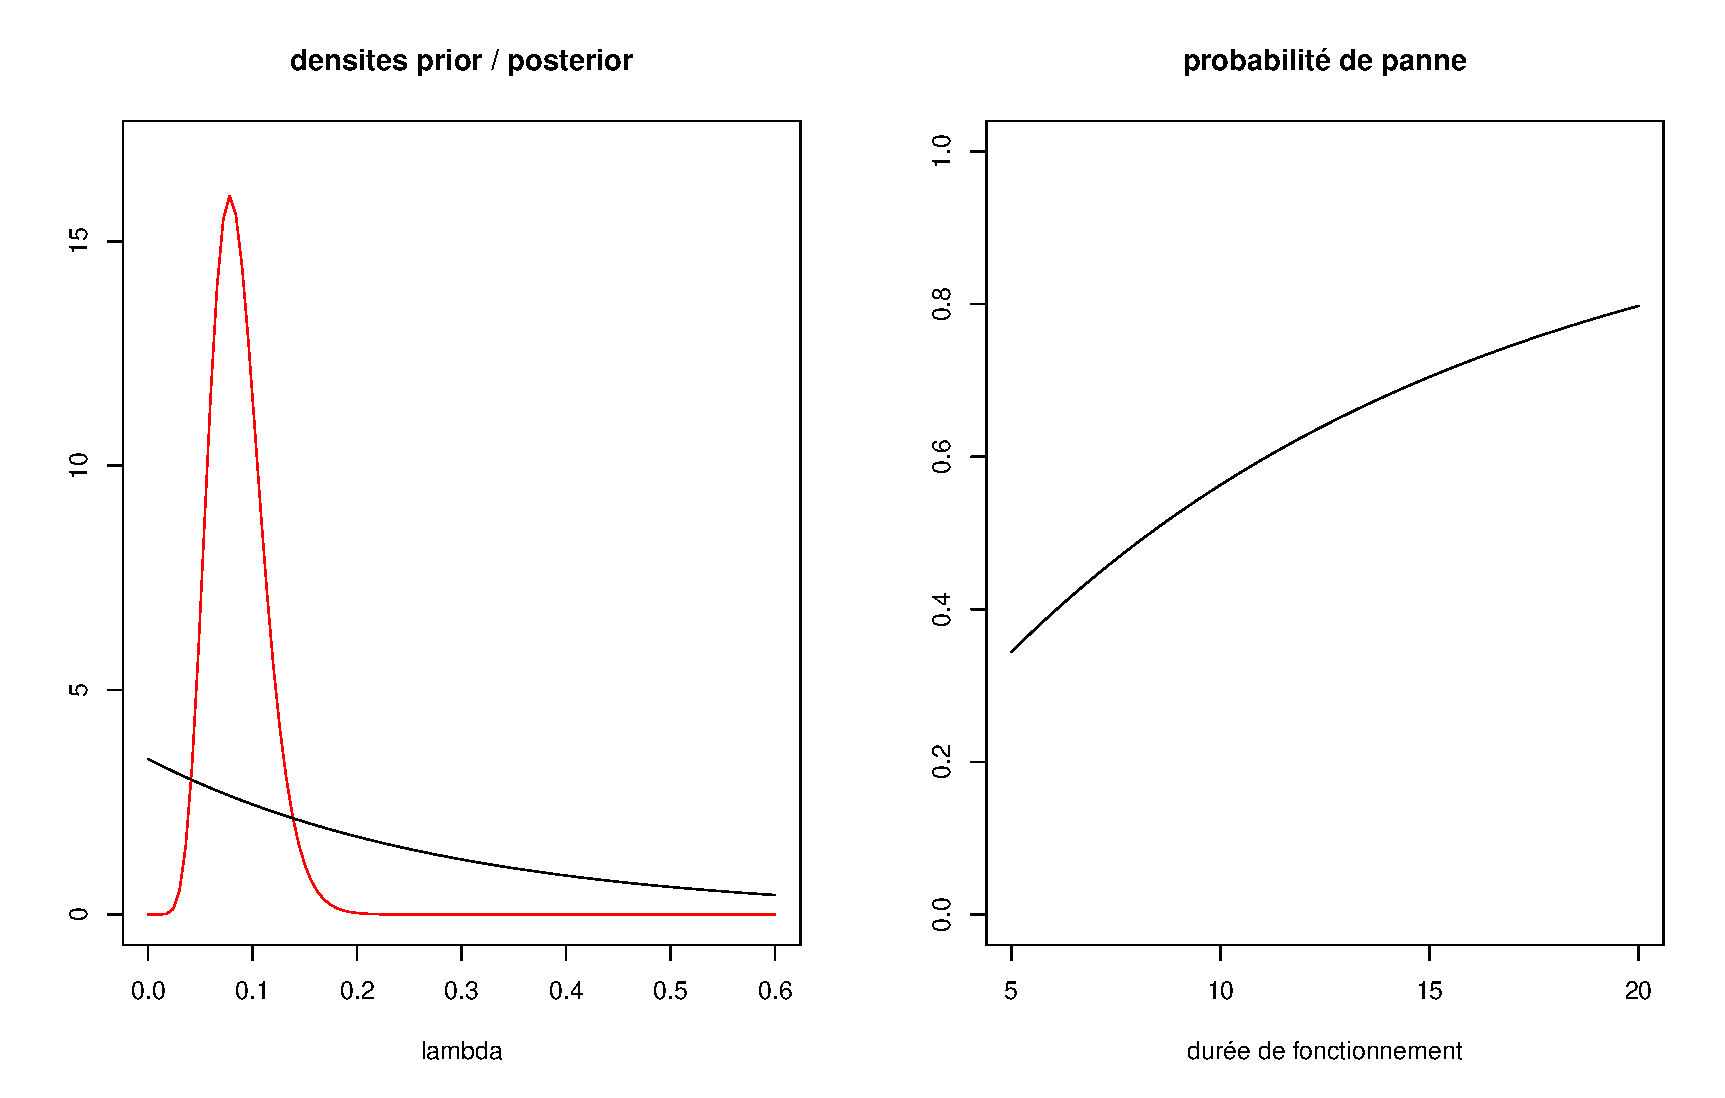
\includegraphics[scale=0.4]{figures/prior/figure01.pdf} 
\caption{$m=1$, $\bar{\lambda}=1/5$, $\alpha=50\%$ (expert peu informatif et pessimiste).}
\label{expert1}
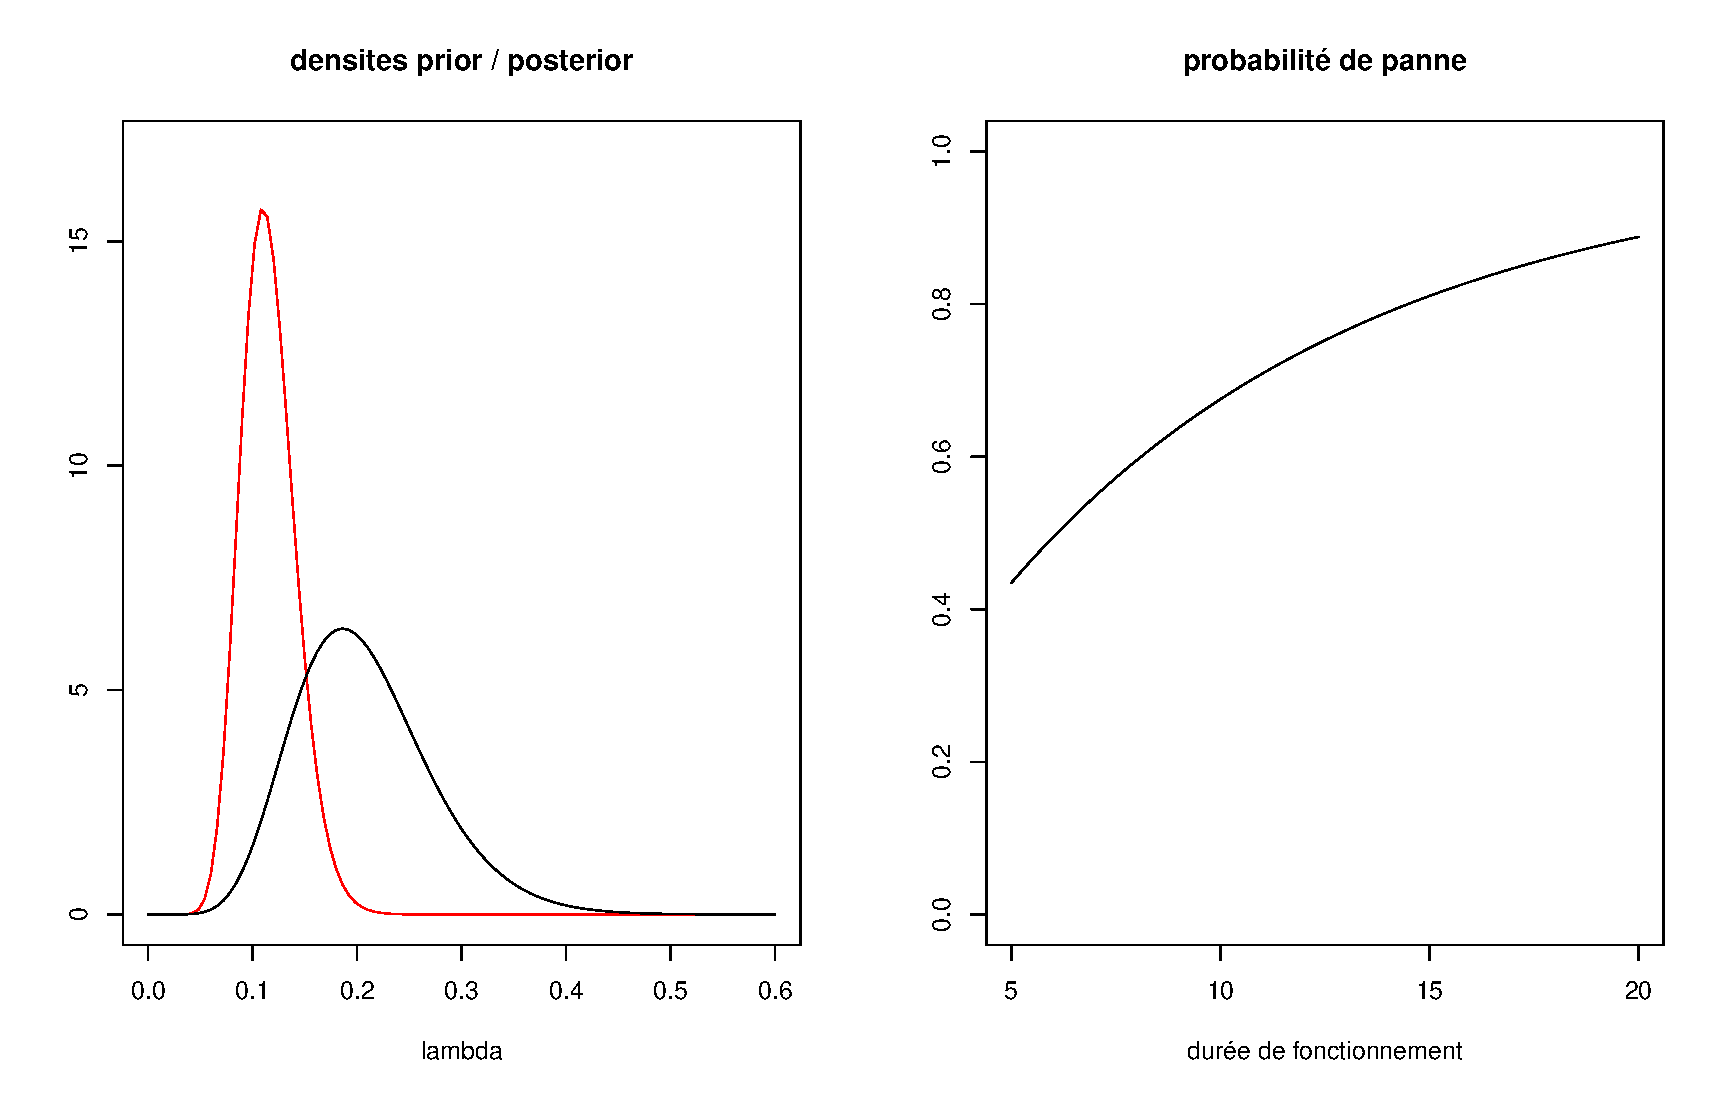
\includegraphics[scale=0.4]{figures/prior/figure02.pdf} 
\caption{$m=10$, $\bar{\lambda}=1/5$, $\alpha=50\%$ (expert très informatif et pessimiste).} \label{expert2}
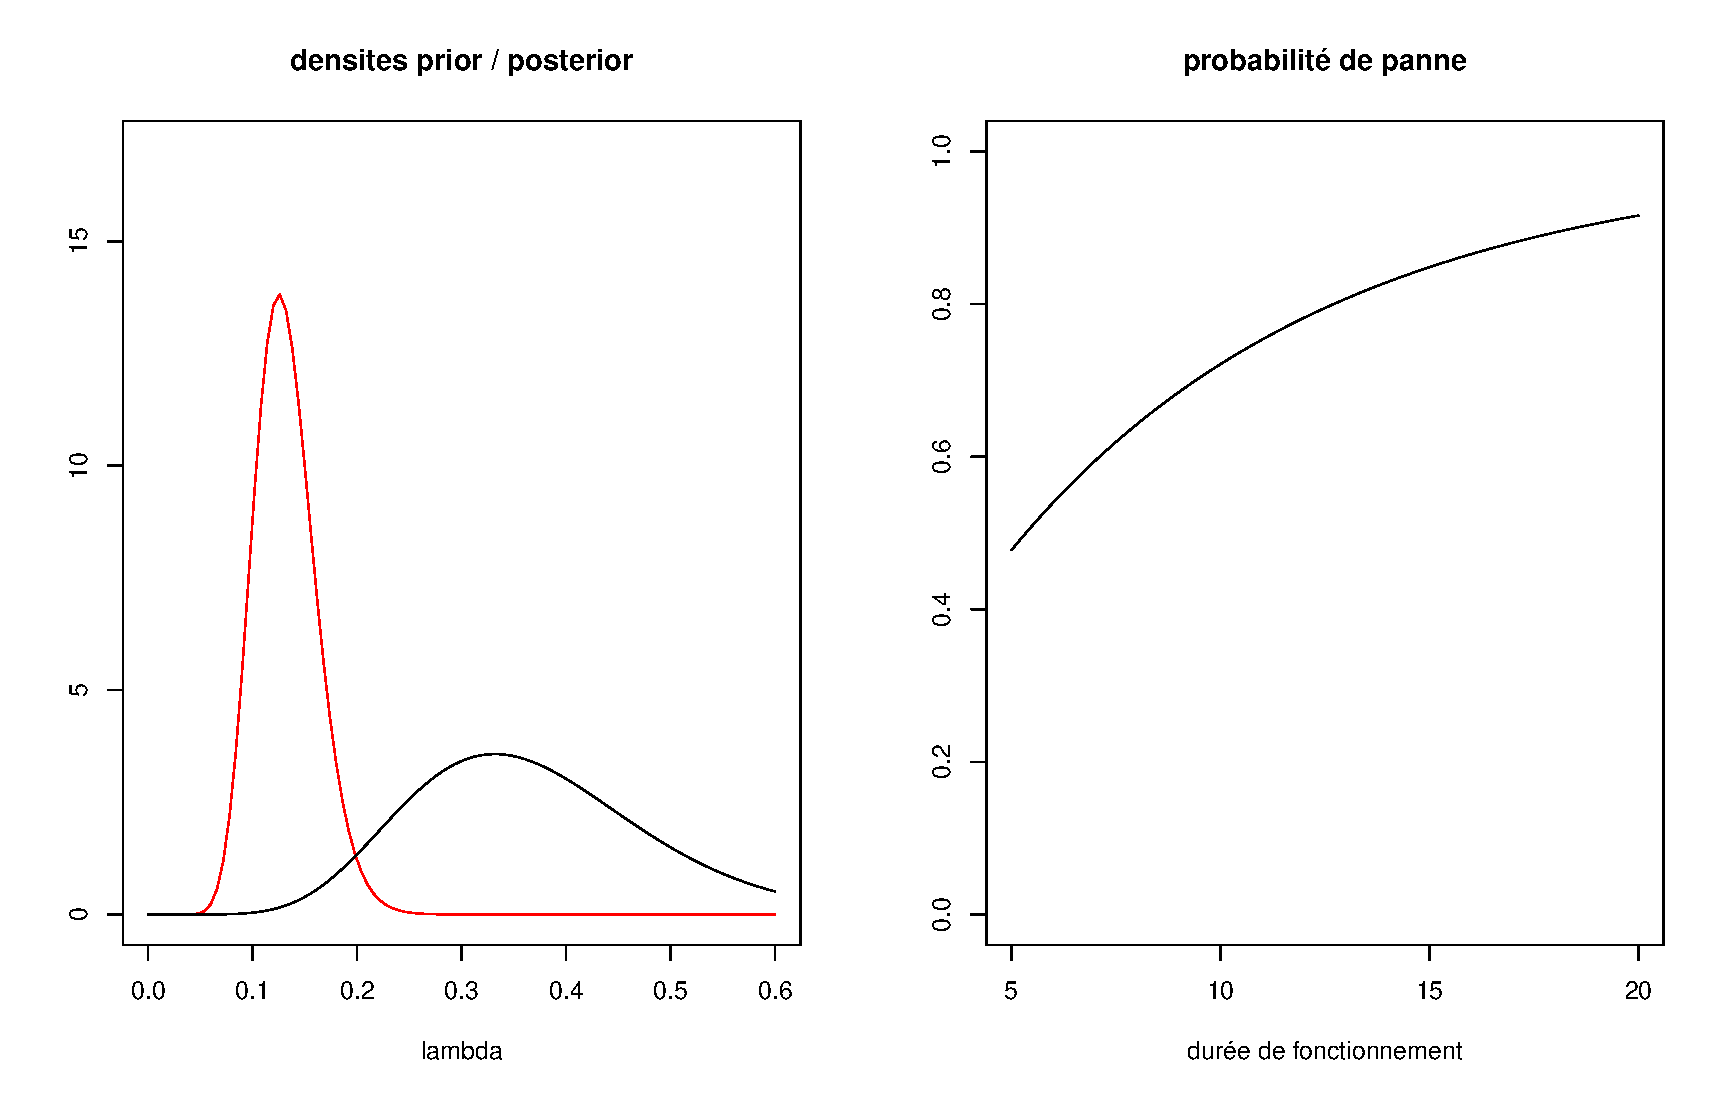
\includegraphics[scale=0.4]{figures/prior/figure03.pdf} 
\caption{$m=10$, $\bar{\lambda}=1/5$, $\alpha=5\%$ (expert très informatif et très pessimiste).} \label{expert3}
\end{figure}

En fait, plus habituellement, l'expert préfère exprimer son opinion \emph{quantitative} sur la durée de vie $X$
 ($=$ \emph{variable d'ancrage}) que sur $\lambda$, car $X$ est {\bf observable}. Dans ce cas, il est assimilé à un fournisseur d'estimé du \emph{quantile prédictif {\it a priori}} $\bar{x}$ :
\begin{eqnarray*}
\int_{0}^{\bar{x}} f(x) \ dx & = & \int_{0}^{\bar{x}} \int_{\Theta} f(x|\theta)\pi(\theta) \ d\theta \ = \ \alpha
\end{eqnarray*}
Cette interprétation est la plus acceptée en général dans la communauté statistique bayésienne, c'est pourquoi les statisticiens fiabilistes préfèrent poser des questions comme : 
\begin{eqnarray*}
\text{\it Sachant les temps $x_0$ et $x_1>x_0$, $\Sigma$ a $1-\alpha$ fois plus de chance de ne pas tomber en panne après $x_0$ qu'après $x_1$.} \\
\text{\it Quelle est votre évaluation de $1-\alpha$ ?} 
\end{eqnarray*}
%\item La réponse est un estimé de $\P(X>x_0)/P(X>x_1)$

\fi



%%%%%%%%%%%%%%%%%%%%%%%%%%%%%%%%%%%%%%%%%%%%%%%%%%%%%%
%%%%%%%%%%%%%%%%%%%%%%%%%%%%%%%%%%%%%%%%%%%%%%%%%%%%%%

\clearpage
\section{Corrigés et preuves "Calcul bayésien"}

%%%%%%%%%%%%%%%%%%%%%%%%%%%%%%%%%%%%%%%%%%%%%%%%%%%%%%
%%%%%%%%%%%%%%%%%%%%%%%%%%%%%%%%%%%%%%%%%%%%%%%%%%%%%%

\subsection{Exercices}

\if\mycmdexotwo1 \vspace{1cm} 
\begin{exec}\label{quasi.conjug}
 On suppose $X   \sim {\cal{N}}(\theta,1)$ et on suppose connaître un échantillon ${\bf x_n}$ composé de :
\begin{itemize}
\item quelques observations $x_1,\ldots,x_{n-1}$ supposées iid. 
\item une pseudo-observation $y$ qui est un cas-limite masquant ({\it censurant}) une observation $x_{n}$ qui aurait dû être faite: $y<x_{n}$
\end{itemize}
 {\it A priori}, on suppose $\theta \sim {\cal{N}}(\mu,1)$. 
Pouvez-vous produire un algorithme d'AR qui génère des réalisations de la loi {\it a posteriori} de $\theta$ ? 
\end{exec}

\begin{rep}% AR
La vraisemblance s'écrit  
\begin{eqnarray*}
f({\bf x_n}|\theta) & \propto & \underbrace{\exp\left(-\frac{1}{2}\sum\limits_{k=1}^{n-1} (x_k-\theta)^2\right)}_{\text{\tiny terme régulier}} \ \ \ \left(\underbrace{1-\Phi(y-\theta)}_{\text{\tiny \begin{tabular}{l} terme dû à la censure \\ $\ \ = \ P(X>y)$ \end{tabular}}}\right).  
\end{eqnarray*}
L'{\it a posteriori} sur $\theta$ s'écrit alors
\begin{eqnarray*}
\pi(\theta|{\bf x_n}) & \propto & \tilde{\pi}(\theta|{\bf x_n}) \ = \ \exp\left\{-\frac{n}{2}\left[\theta - \frac{1}{n}\left(\mu + \sum\limits_{k=1}^{n-1} x_k\right)\right]^2\right\}\left\{1-\Phi(y-\theta)\right\}. 
\end{eqnarray*}
On remarque que si $y=x_n$, on aurait un modèle conjugué et $\pi(\theta|{\bf x_n})$ serait une loi normale. Il semble donc pertinent de proposer, comme choix de loi instrumentale,
$$
\rho(\theta) \equiv {\cal{N}}\left(\frac{1}{n}\left(\mu + \sum\limits_{k=1}^{n-1} x_k\right),1/n\right).
$$
Puisque $1-\Phi(y-\theta)\leq 1$, on a
\begin{eqnarray*}
\tilde{\pi}(\theta|{\bf x_n}) & \leq & \underbrace{\sqrt{\frac{2\pi}{n}}}_{K} \cdot\{1-\Phi(y-\theta)\}\cdot\rho(\theta).
\end{eqnarray*}
On peut donc mettre en oeuvre l'algorithme comme suit : on accepte $\theta_i$ si $U_i\leq 1-\Phi(y-\theta_i)$. Le nombre moyen d'appels nécessaires à $\rho(\theta)$ varie proportionnellement à $1/\sqrt{n}$, donc
plus l'échantillon de données grandit, plus l'algorithme est efficace.
Si cependant, on fait le choix $\rho(\theta)=\pi(\theta)$, alors
\begin{eqnarray*}
K & = & \sqrt{2\pi}\exp\left(\frac{1}{2}\left[\frac{1}{n-1}\sum\limits_{k=1}^n x_k - \mu\right](1-\sqrt{n})\right) 
\end{eqnarray*}
Voir la figure \ref{ARillus} pour une illustration de la mise en oeuvre de cet algorithme.
\end{rep}

\begin{figure}[hbtp]
\begin{center}
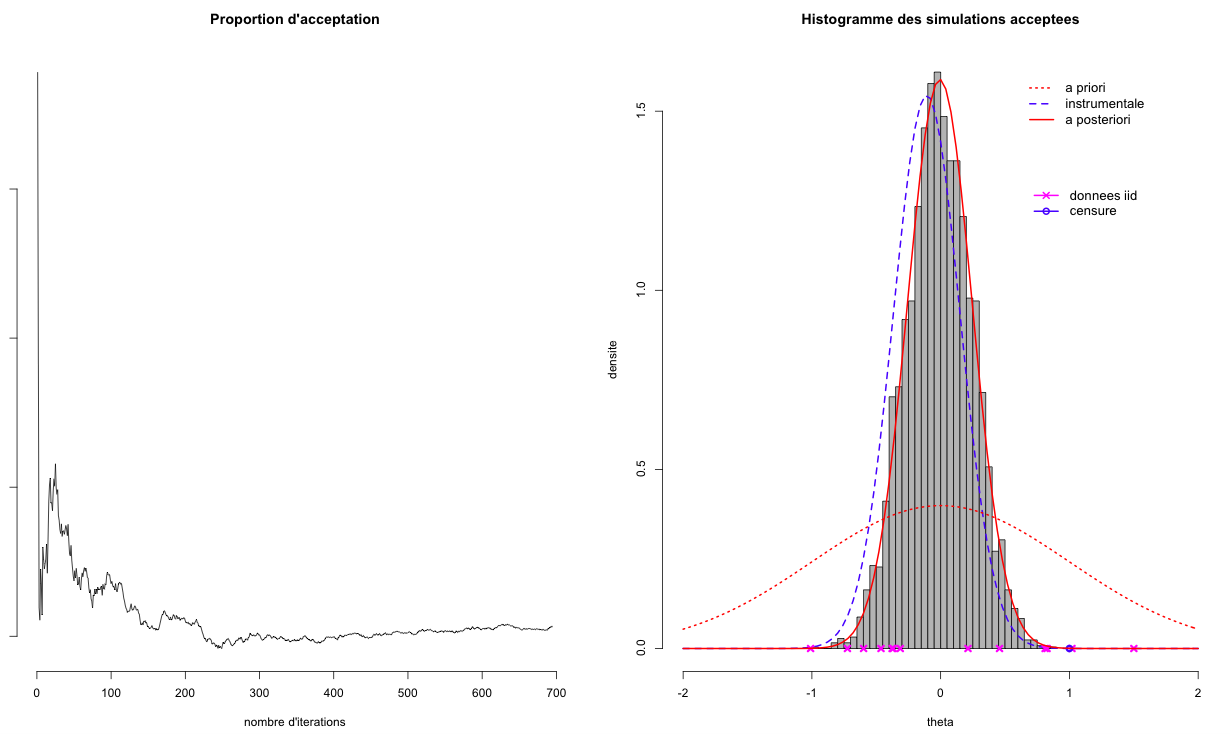
\includegraphics[scale=0.3]{figures/calcul/AR1.png} \\
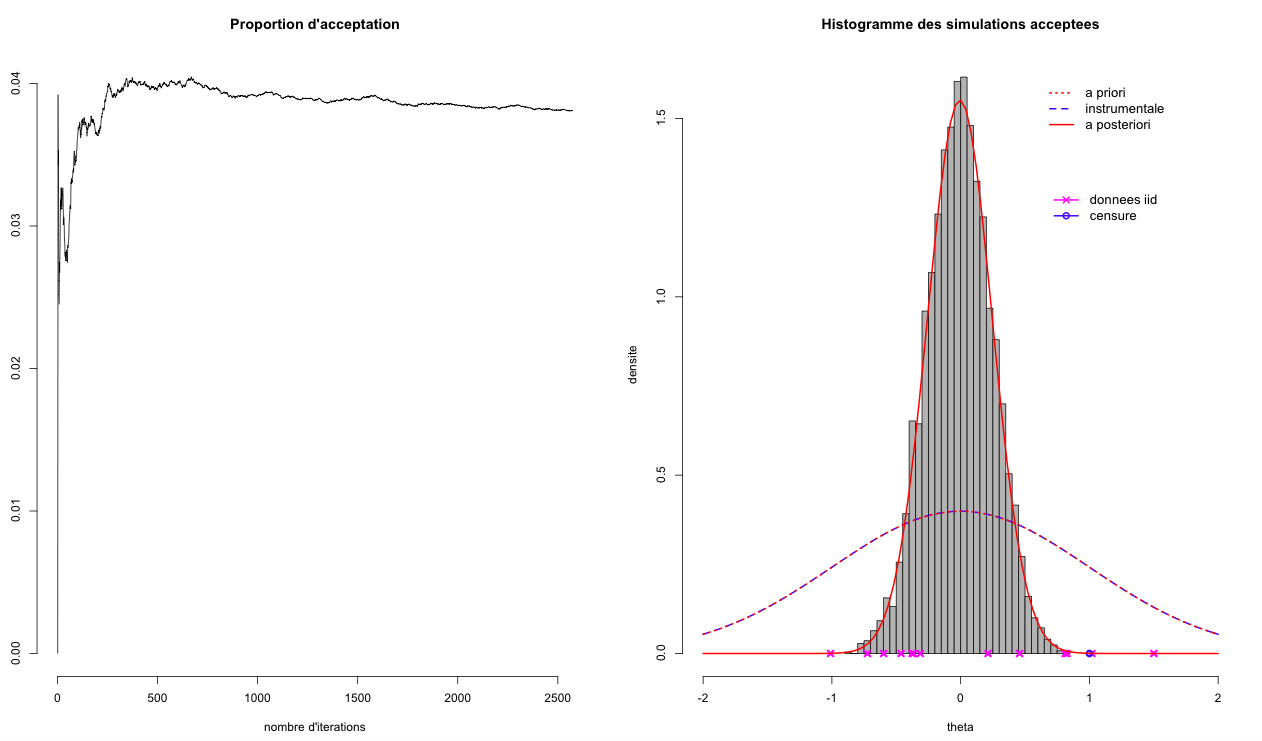
\includegraphics[scale=0.3]{figures/calcul/AR2.png}
\caption{
Essai de simulation par AR en utilisant (en haut) une loi instrumentale ``proche" du vrai posterior ; (en bas) le prior comme loi instrumentale.}
\label{ARillus}
\end{center}
\end{figure}

\clearpage
\fi

\if\mycmdexotwo1 \vspace{1cm}
\begin{exec}\label{gamma}
Soit un échantillon de loi gamma $x_1,\ldots,x_n\overset{iid}{\sim} {\cal{G}}(a,\theta)$ où $a$ est connu. On suppose $\pi(\theta)\equiv {\cal{G}}(c,d)$. Produisez une méthode par AR pour simuler la loi {\it a posteriori} $\pi(\theta|x_1,\ldot,x_n)$ et vérifiez que les tirages obtenus sont bien issus de cette loi, par ailleurs explicite.
\end{exec}

 \begin{rep}
Il est aisé de vérifier qu'on connaît parfaitement la loi {\it a posteriori} de $\theta$ :
\begin{eqnarray*}
\theta|x_1,\ldots,x_n %& \sim & \pi(\theta|x_1,\ldots,x_n) \ \propto \ \\
& \sim & {\cal{G}}\left(c+an,d+\sum\limits_{i=1}^n x_i\right).
\end{eqnarray*}
On peut donc vérifier l'accord entre un échantillon iid simulé par AR et cette loi, via des tests statistiques classiques comme Kolmogorov-Smirnov, Cramer-von Mises ou Anderson-Darling. Pour construire cet algorithme d'AR, faisons par exemple le choix d'une loi instrumentale lognormale (qui est bien à support positif, car $\theta>0$) :
\begin{eqnarray*}
\rho(\theta|\mu,\sigma) & = & \frac{1}{\theta\sigma \sqrt{2\pi}} \exp\left(-\frac{1}{2\sigma^2}\left(\mu-\log\theta\right)^2\right).
\end{eqnarray*}
Il vient alors 
\begin{eqnarray*}
\kappa(\theta|\mu,\sigma)  \ = \  \frac{f(x_1,\ldots,x_n|\theta)\pi(\theta)}{\rho(\theta)} & = & {\displaystyle \frac{\sqrt{2\pi} \sigma \theta^{c+an} \exp\left(-\theta(d+\sum_{i=1}^n x_i)\right)}{\exp\left(-\frac{1}{2\sigma^2}\left(\mu-\log\theta\right)^2\right)}}
\end{eqnarray*}
et 
\begin{eqnarray*}
\frac{\partial }{\partial \theta} \log \kappa(\theta|\mu,\sigma) & = & \frac{c+an}{\theta} - \left(d+\sum\limits_{i=1}^n x_i\right) - \frac{1}{\sigma^2\theta}\left(\mu-\log(\theta)\right), \\
\frac{\partial^2 }{\partial \theta^2} \log \kappa(\theta|\mu,\sigma) & = & \frac{1}{\theta^2}\left(-(c+an) + \frac{1}{\sigma^2}(1+\mu - \log(\theta)\right).
\end{eqnarray*}
Notons $\theta_0(\mu,\sigma)=\exp(-(c+an)+(1+\mu)/\sigma^2)$. Si $0\leq \theta\leq \theta_0$, alors $\frac{\partial }{\partial \theta} \log \kappa(\theta|\mu,\sigma)$ est croissante. Si $\theta>\theta_0$, elle est décroissante vers $-(d+\sum_{i=1}^n x_i)<0$. Pour permettre à $\kappa(\theta|\mu,\sigma)$ d'être maximisable sur $\theta>0$, il faut donc que 
$$
\frac{\partial }{\partial \theta} \log \kappa(\theta_0(\mu,\sigma)|\mu,\sigma) = -\left(d+\sum\limits_{i=1}^n x_i\right) + 1/\sigma^2\theta_0 \ > \ 0.
$$
Sous cette contrainte, on peut résoudre numériquement en $\theta=\theta_1(\mu,\sigma)>\theta_0(\mu,\sigma)$ l'équation $\frac{\partial }{\partial \theta} \log \kappa(\theta|\mu,\sigma)=0$, et $\theta_1(\mu,\sigma)$ maximise alors $\kappa(\theta|\mu,\sigma)$. Dans ce cas, on peut définir 
\begin{eqnarray*}
K & = & \arg\min\limits_{\mu,\sigma} \kappa(\theta_1(\mu,\sigma)|\mu,\sigma). 
\end{eqnarray*}
et mettre en place l'algorithme AR.
\end{rep}
\fi

\if\mycmdexotwo1 \vspace{1cm} 
\begin{exec}
Considérons une fonction d'intérêt $h(\theta)$ que l'on cherche à résumer par un estimateur calculé sous un coût quadratique ; il s'agit donc de l'espérance {\it a posteriori}
\begin{eqnarray}
h \ = \ \E_{\pi}[h(\theta)|x_1,\ldots,x_n] & = & \int_{\Theta} h(\theta)\pi(\theta|x_1,\ldots,x_n) \ d\theta\label{IS.estim1}
\end{eqnarray}
que l'on suppose pouvoir estimer simplement, de fa\c con consistante, par Monte Carlo. Supposons vouloir modifier le prior : $\pi(\theta)\to\pi'(\theta)$, sans modifier le support, mais de fa\c con à ce que la nouvelle loi {\it a posteriori} ne soit plus directement simulable. Peut-on (et sous quelles conditions) ne pas faire de calcul supplémentaire pour simuler le nouveau posterior $\pi'(\theta\x_1,\ldots,x_n)$ ?
\end{exec}

\begin{rep}
On considére donc une fonction d'intérêt $h(\theta)$ que l'on cherche à résumer par son espérance {\it a posteriori}
\begin{eqnarray}
h \ = \ \E_{\pi}[h(\theta)|x_1,\ldots,x_n] & = & \int_{\Theta} h(\theta)\pi(\theta|x_1,\ldots,x_n) \ d\theta\label{IS.estim1}
\end{eqnarray}
que l'on suppose pouvoir estimer simplement, de fa\c con consistante, par Monte Carlo :
\begin{eqnarray*}
\hat{h}_M & = & \frac{1}{M}\sum\limits_{k=1}^M h(\theta_i) \ \ \ \text{avec $\theta_i\overset{iid}{\sim} \pi(\theta|x_1,\ldots,x_n)$}
\end{eqnarray*}
Supposons vouloir modifier le prior : $\pi(\theta)\to\pi'(\theta)$, sans modifier le support, mais de fa\c con à ce que la nouvelle loi {\it a posteriori} ne soit plus directement simulable. En supposant que $\pi(\theta|x_1,\ldots,x_n)>0$ pour tout $\theta\in\Theta$, on peut néanmoins recalculer facilement le nouvel estimateur de Bayes :
\begin{eqnarray*}
h' \ = \ \E_{\pi'}[h(\theta)|x_1,\ldots,x_n] & = & \int_{\Theta} h(\theta)\pi'(\theta|x_1,\ldots,x_n) \ d\theta, \\
& = & \int_{\Theta} \omega(\theta_i) h(\theta)\pi(\theta|x_1,\ldots,x_n) \ d\theta
\end{eqnarray*}
avec
\begin{eqnarray*}
\omega(\theta_i) & = & \frac{\pi'(\theta|x_1,\ldots,x_n) }{\pi(\theta|x_1,\ldots,x_n)} \ = \ C\tilde{\omega}^*_i 
\end{eqnarray*}
où 
\begin{eqnarray*}
\tilde{\omega}^*_i  & = & \left(\frac{\pi'(\theta_i)}{\pi(\theta_i)}\right), \\
C & = &  \frac{m_{\pi}(x_1,\ldots,x_n)}{m_{\pi'}(x_1,\ldots,x_n)}.
\end{eqnarray*}
Le calcul de la constante de proportionnalité $C$ nécessiterait usuellement de disposer de deux échantillons {\it a posteriori}. On peut cependant s'en passer en remarquant que d'après la loi forte des grands nombres,  \begin{eqnarray*}
\frac{1}{M}\sum\limits_{i=1}^M \tilde{\omega}^*_i & \xrightarrow[n\to \infty]{p.s.} & \frac{1}{C}\int_{\Theta} \omega(\theta) \pi(\theta|x_1,\ldots,x_n) \ d\theta \ = \ 1/C
\end{eqnarray*}
et on en déduit donc qu'un estimateur IS  consistant de $h'$,  qui réutilise les calculs faits pour l'estimateur $\hat{h}_M$  sans coût calculatoire additionnel, est 
\begin{eqnarray*}
\hat{h''}_M & = & \frac{1}{M}\sum\limits_{k=1}^M \hat{\omega}^*_i h(\theta_i)
\end{eqnarray*}
avec
\begin{eqnarray*}
\hat{\omega}^*_i & = & \frac{\tilde{\omega}^*_i}{\sum\limits_{j=1}^M \tilde{\omega}^*_j}.
\end{eqnarray*}

 %\left(\frac{\pi'(\theta)}{\pi(\theta)}\right) \left(\frac{m_{\pi}(x_1,\ldots,x_n)}{m_{\pi'}(x_1,\ldots,x_n)}\right)
%\end{eqnarray*}
%Le second terme entre parenthèses ne dépend pas de $\theta$. En faisant l'hypothèse suivante :
%\begin{eqnarray*}
%\forall i\in\{1,\ldots,M\}, \ \ \pi(\theta_i_>0, \label{prior.pos}
%\end{eqnarray*}
%on peut donc proposer l'estimateur IS suivant pour $h'$, qui réutilise les calculs faits pour l'estimateur $\hat{h}_M$ : 
%\begin{eqnarray*}
%\hat{h'}_M & = & \frac{1}{M}\sum\limits_{k=1}^M \tilde{\omega}_i h(\theta_i)
%\end{eqnarray*}
%avec
%\begin{eqnarray*}
%\tilde{\omega}_i  =  C\tilde{\omega}^*_i & \text{et} & 
%\tilde{\omega}^*_i  =  \left(\frac{\pi'(\theta_i)}{\pi(\theta_i)}\right),
%\end{eqnarray*}
%et $C$ la constante de proportionnalité 
%\begin{eqnarray*}
%C & = & \frac{m_{\pi}(x_1,\ldots,x_n)}{m_{\pi'}(x_1,\ldots,x_n)}
%\end{eqnarray*}
%dont le calcul nécessite en théorie uniquement des tirages des deux priors (par Monte Carlo). Cependant, on remarque que par la loi forte des grands nombres, que 
%\begin{eqnarray*}
%\frac{1}{M}\sum\limits_{i=1}^M \tilde{\omega}^*_i & \xrightarrow[n\to \infty]{p.s.} & 
%\end{eqnarray*}

%On remarque, par la loi forte des grands nombres,  que

%\E\left[\frac{1}{M}\sum\limits_{i=1}^M \tilde{\omega}^*_i\right] \ = \ \frac{1}{M}\sum\limits_{i=1}^M \int_{\Theta} \pi'(\theta) \ d\theta \ = \ 1.
%\end{eqnarray*}
%Cependant, on sait que le calcul par Monte Carlo selon des tirages {\it a priori} du rapport $C$ des lois marginales peut être fortement instable. Il est donc simplement conseillé d'adopter la démarche suivante, suivant le théorème \ref{SIR.rubin} :
%\begin{enumerate}
%\item calculer les poids relatifs $\tilde{\omega}^*_i$ ;
%\item resimuler avec remise dans $\theta_1,\ldots,\theta_M$ selon les poids $\tilde{\omega}^*_i$ pour obtenir de nouveaux tirages {\it a posteriori} de $\pi'(\theta|x_1,\ldots,x_n)$. 
%\end{enumerate}
Notons que ce faisant, on crée de la corrélation entre les deux estimateurs de $h$. 
\end{rep}
\fi

\if\mycmdexotwo1 \vspace{1cm}
\begin{exec}\label{debit.extreme}
Soit $X$ la variable ``débit maximal de rivière". Elle est supposée suivre une loi des extrêmes (Gumbel) de densité
\begin{eqnarray*}
f(x|\theta) & = &  \lambda\mu\exp(-\lambda x)
\exp(-\mu\exp(-\lambda x)).
\end{eqnarray*}
avec $\theta=(\mu,\lambda)$. %L'espérance est
%\begin{eqnarray*}
%\E[X|\theta] & = & \lambda^{-1}\left(\log \mu + \gamma\right)
%\end{eqnarray*}
%où $\gamma$ est la constante d'Euleur ($\simeq$ 0.578..)
\begin{center}
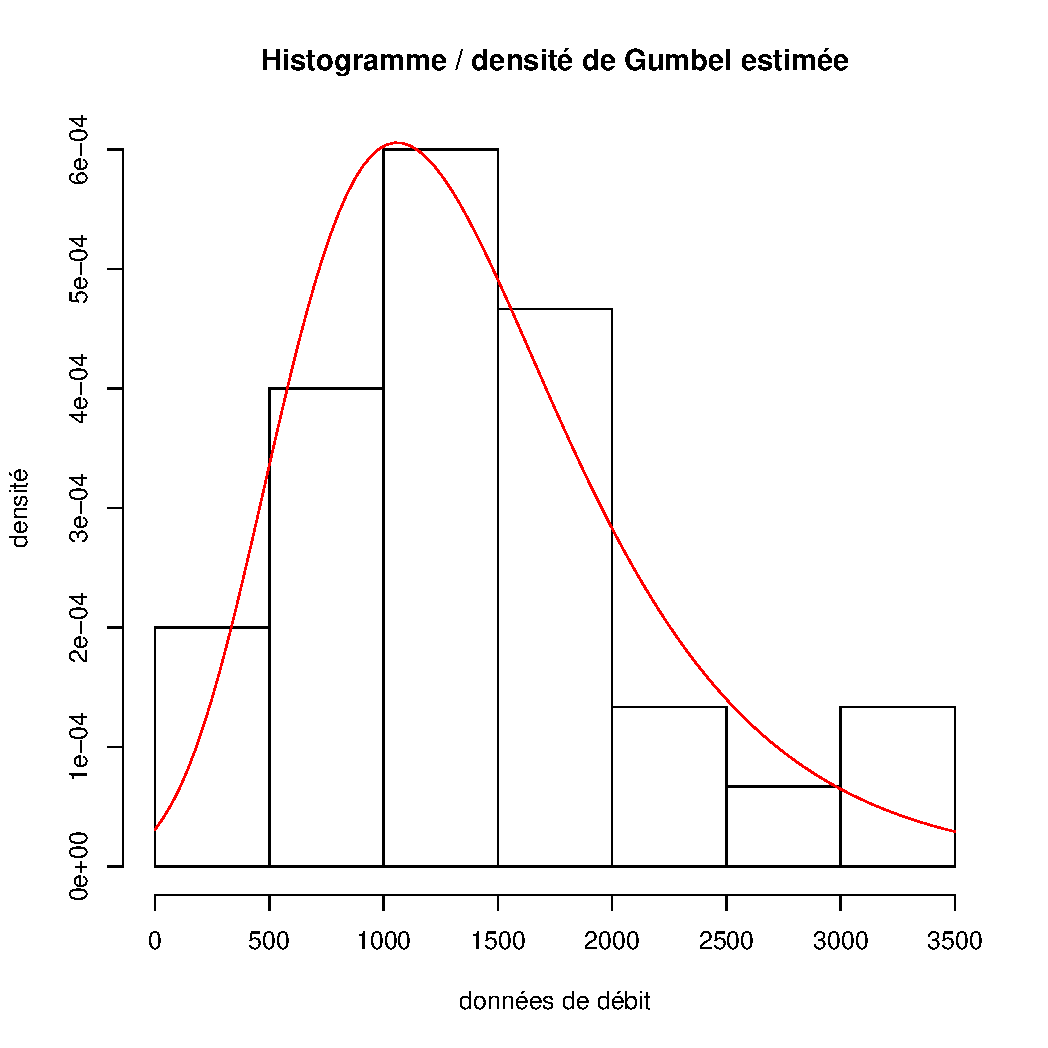
\includegraphics[scale=0.4]{figures/calcul/hist-gumbel.pdf}
\end{center}
Considérons $n$ observations ${\bf x_n}=(x_1,\ldots,x_n)$ supposées iid  selon cette distribution. 
\begin{enumerate}
    \item Comment s'écrit la vraisemblance ?
    \item On considère l'{\it a priori} $\pi(\mu,\lambda) = \pi(\mu|\lambda)\pi(\lambda)$ avec
\begin{eqnarray*}
\mu|\lambda & \sim   & {\cal{G}}\left(m,b_m(\lambda) \right),  \\
\lambda    & \sim   & {\cal{G}}\left(m,m/\lambda_e\right)
\end{eqnarray*}
et ${\displaystyle b_m(\lambda)  = \left[\alpha^{-1/m}
-1\right]^{-1} \exp(-\lambda x_{e,\alpha}).}$. Ces hyperparamètres ont le sens suivant :
\begin{itemize}
\item $x_{e,\alpha}=$ quantile prédictif {\it a priori} d'ordre $\alpha$:
\begin{eqnarray*}
P\left(X<x_{e,\alpha}\right) & = & \int P\left(X<x_{e,\alpha}|\mu,\lambda\right)  \pi(\mu,\lambda) \ d\mu d\lambda \ = \ \alpha ; 
\end{eqnarray*}  
\item $m =$ taille d'échantillon fictif, associée à la ``force" de la connaissance {\it a priori} $x_{e,\alpha}$ ; 
\item $1/\lambda_e = $ moyenne de cet échantillon  fictif. 
\end{itemize}
Pouvez-vous produire un algorithme de type MCMC qui permette de générer une loi jointe {\it a posteriori} pour $(\mu,\lambda)$ ? 
\end{enumerate}
\end{exec}

 \begin{rep}
En posant
%\begin{eqnarray*}
$\bar{x}_n  =  \frac{1}{n}\sum\limits_{i=1}^n x_i$ et 
$\bar{b}_{{\bf x_n}}(\lambda)  =  \sum\limits_{i=1}^n \exp\left(-\lambda x_i\right)$, 
la vraisemblance s'écrit alors
\begin{eqnarray*}
f\left({\bf x_n}\right) & = & \lambda^n \mu^n \exp(-\lambda n\bar{x}_n) \exp\{-\mu\bar{b}_{{\bf x_n}}(\lambda)\}.
\end{eqnarray*}
En conséquence, la loi {\it a posteriori} s'obtient sous la forme \emph{hiérarchisée} suivante :
\begin{eqnarray*}
\pi\left(\mu,\lambda|{\bf x_n}\right) & = & \pi\left(\mu|\lambda,{\bf x_n}\right) \pi\left(\lambda|{\bf x_n}\right)
\end{eqnarray*}
où
\begin{eqnarray*}
\mu|\lambda,{\bf x_n} & \sim & {\cal{G}}\left(m+n,b_m(\lambda) + \bar{b}_{{\bf x_n}}(\lambda)\right)
\end{eqnarray*}
et
\begin{eqnarray*}
\pi\left(\lambda|{\bf x_n}\right) & =  & %\underbrace{\propto}_{\text{\tiny proportionnel}} &  
\gamma(\lambda)\cdot {\cal{G}}\left(m+n,{m}/{\lambda_e} + n\bar{x}_n\right)
%\frac{\left(b_m(\lambda)\right)^m}{\left(b_m(\lambda) + \bar{b}_{{\bf x_r},{\bf c_{n-r}}}(\lambda)\right)^{m+r}} \lambda^{m+r-1} \exp\left(-\lambda ({m}/{\lambda_e} + r\bar{x}_r) \right)
\end{eqnarray*}
avec
\begin{eqnarray*}
\gamma(\lambda) & \propto & \frac{b^m_m(\lambda)}{ \left(b_m(\lambda) + \bar{b}_{{\bf x_n}}(\lambda)\right)^{m+n}}
\end{eqnarray*}
La loi {\it a priori} est donc \emph{semi-conjuguée}, et il suffit de simuler $\lambda$ {\it a posteriori} pour obtenir un tirage joint {\it a posteriori} de $(\mu,\lambda)$. On trace ci-dessous quelques graphiques typiquement obtenus. Plusieurs choix de lois instrumentales pour $\rho(\lambda|\lambda^{(i-1)})$ peuvent être faits. On peut notamment proposer : 
\begin{itemize}
\item la loi {\it a priori} $\pi(\lambda)$ ; 
\item une loi qui ``semble proche": ${\cal{G}}\left(m+n,{m}/{\lambda_e} + n\bar{x}_n\right)$ ; 
\item une loi normale de moyenne $\lambda^{(i-1)}$ et de coefficient de variation petit (5\%) ou grand (25 ou 50\%).
\end{itemize}


\begin{center}
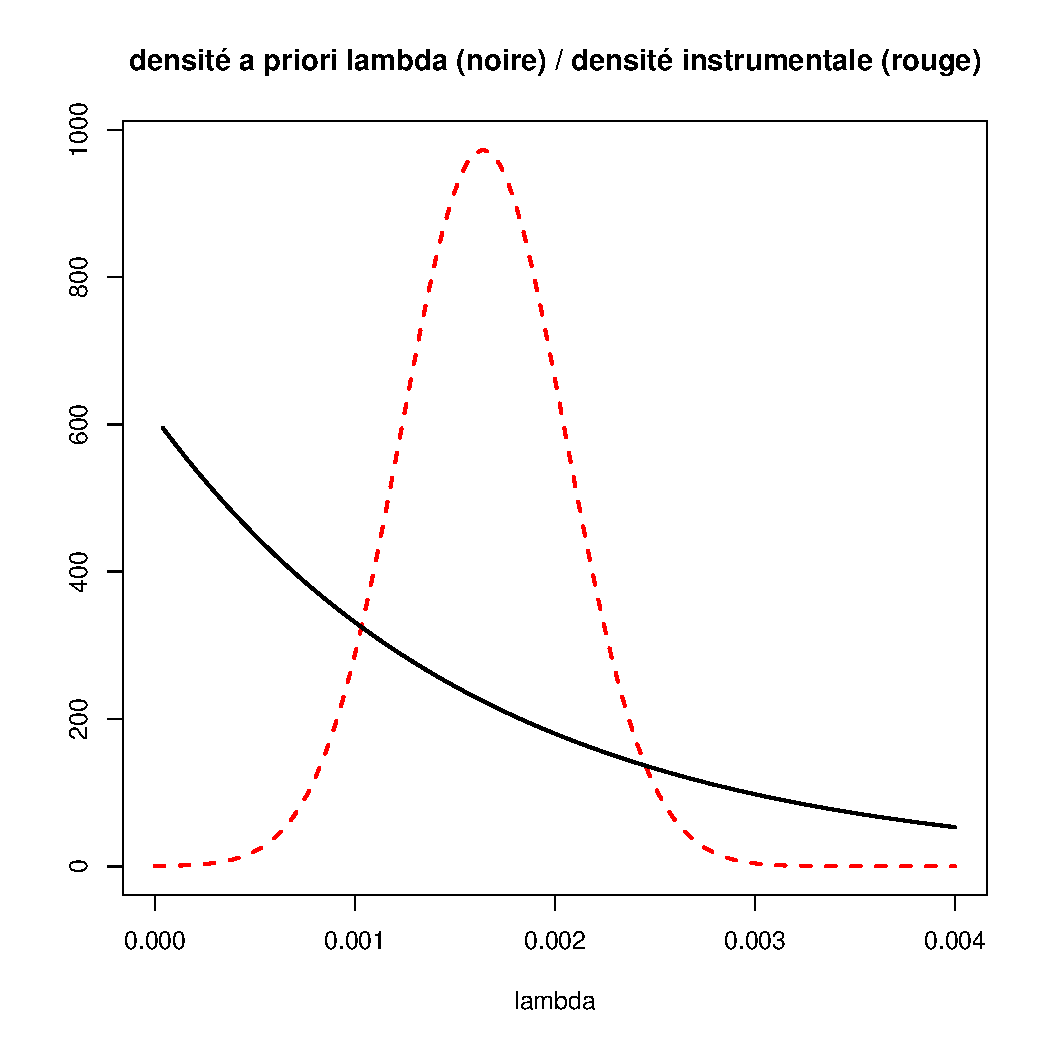
\includegraphics[width=6cm,height=5cm]{figures/calcul/prior-1.pdf} 
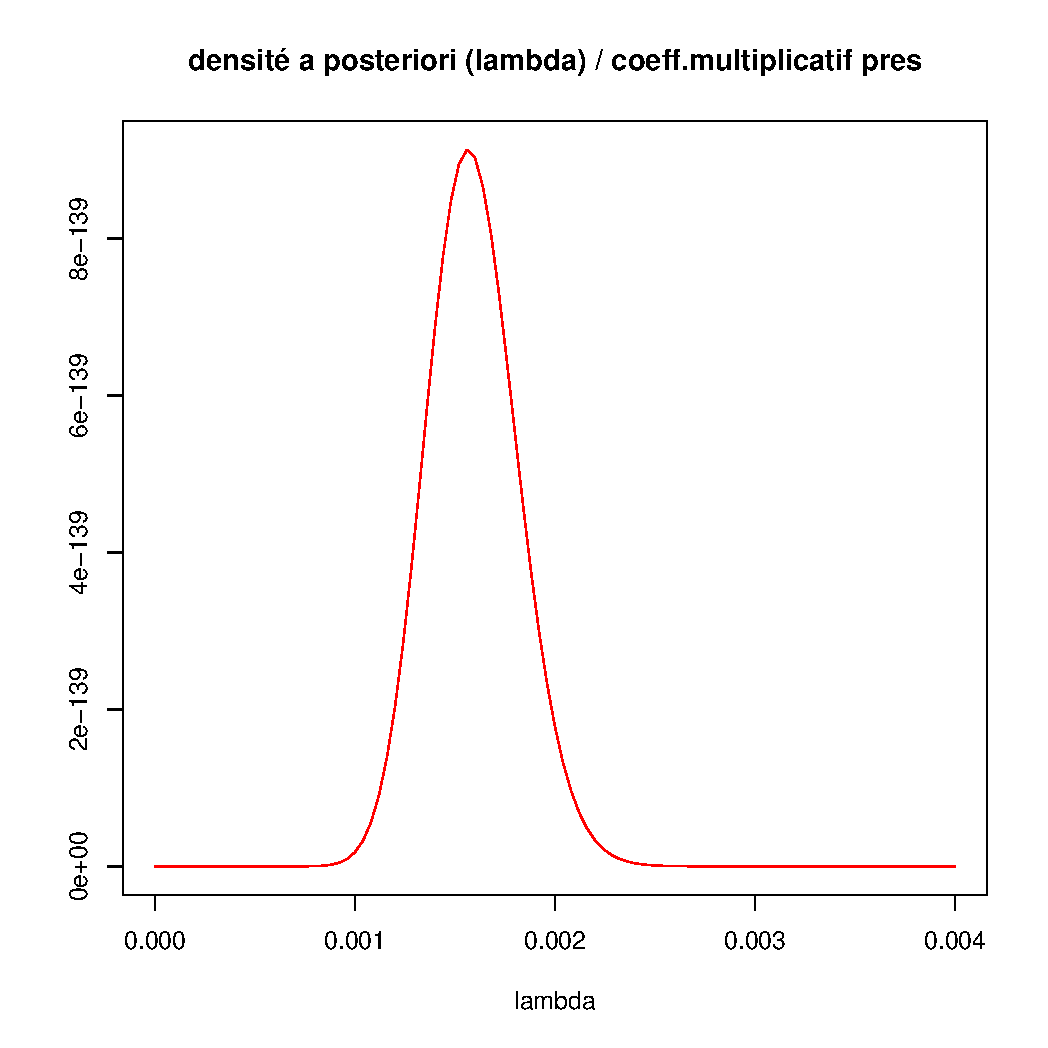
\includegraphics[width=6cm,height=5cm]{figures/calcul/posterior-1.pdf} \\
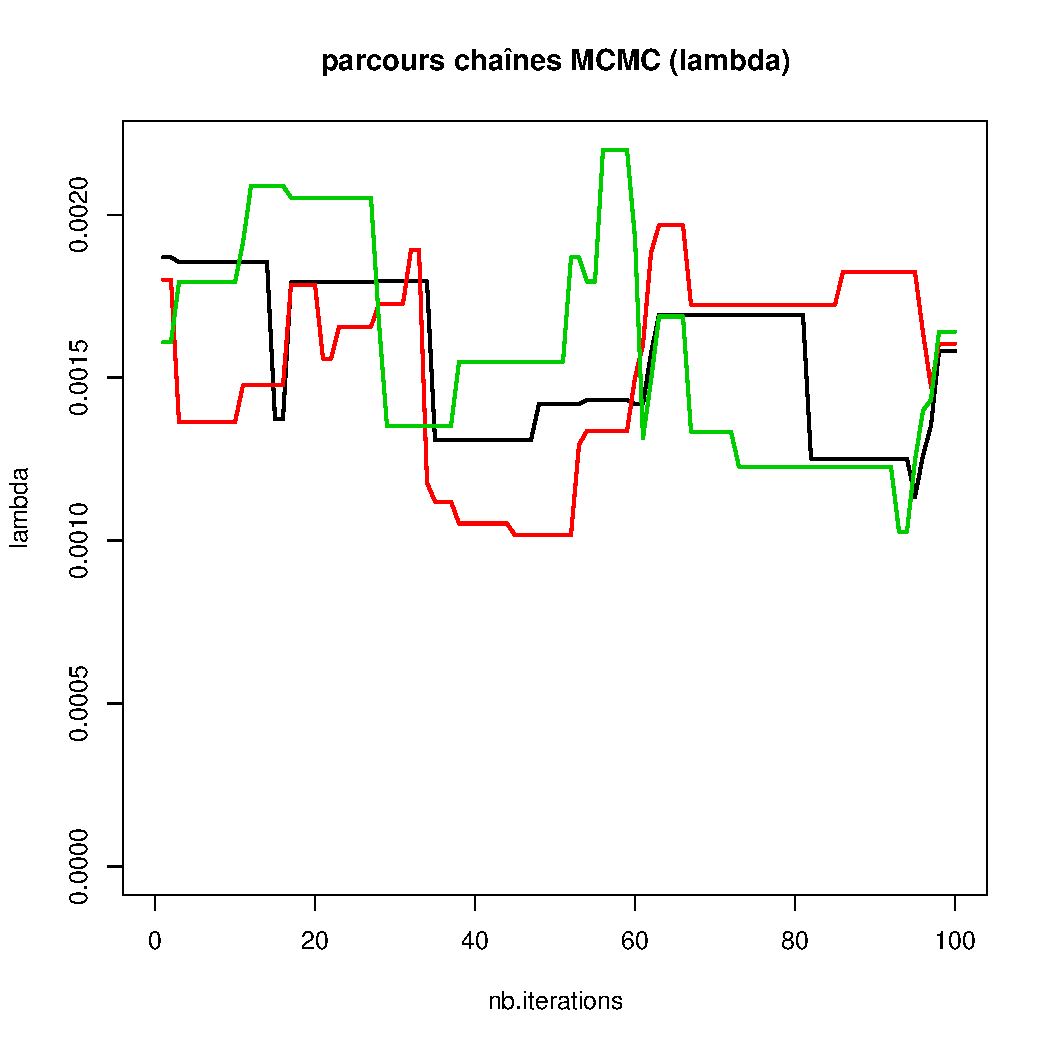
\includegraphics[width=6cm,height=5cm]{figures/calcul/MCMC1.pdf}
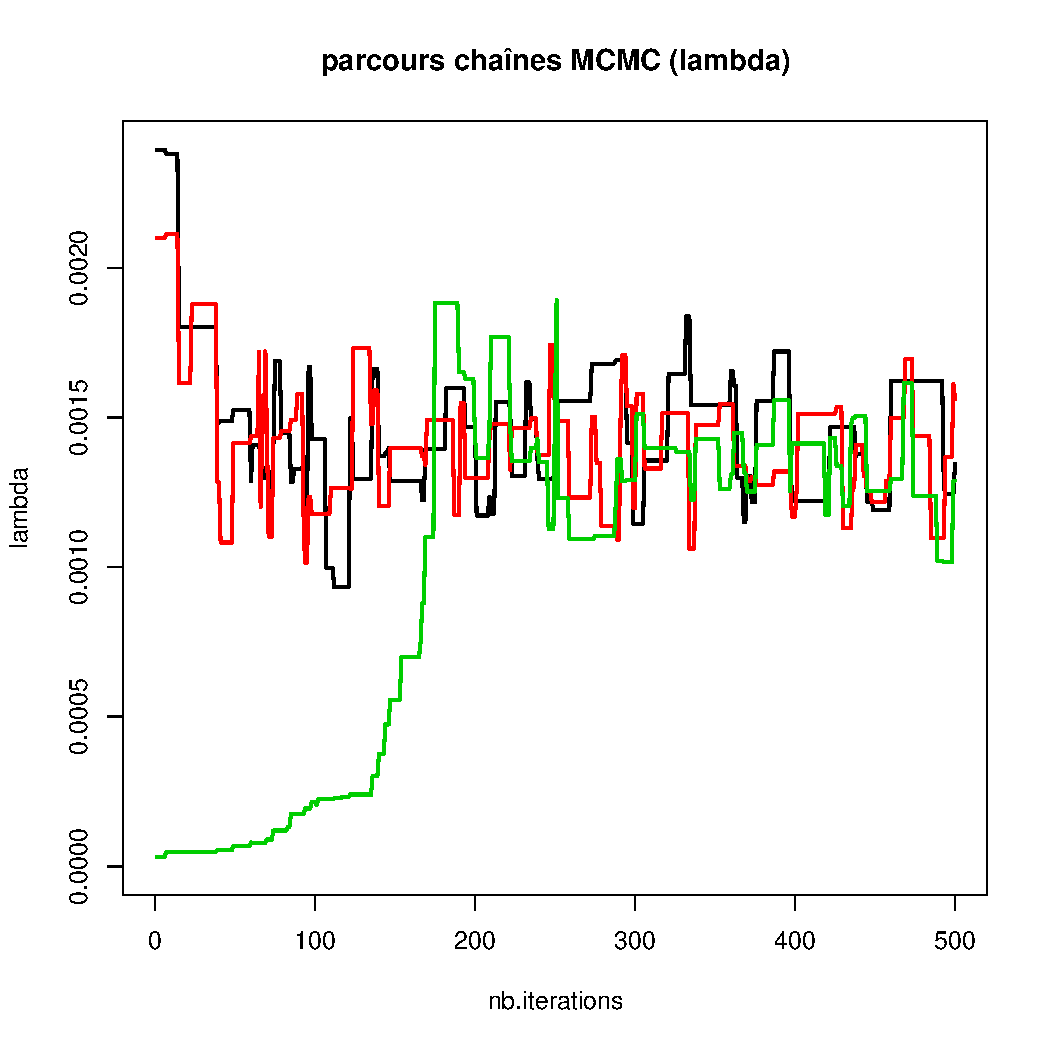
\includegraphics[width=6cm,height=5cm]{figures/calcul/MCMC2.pdf}
\end{center}
\end{rep}
\fi

\if\mycmdexotwo1 \vspace{1cm}
\begin{exec}{\bf (Retour à l'exercice \ref{quasi.conjug}).}. 
 On suppose de nouveau connaître un échantillon ${\bf x_n} \sim {\cal{N}}(\theta,1)$ composé de quelques observations $x_1,\ldots,x_{n-1}$ supposées iid de loi ${\cal{N}}(\theta,1)$, et d'une  pseudo-observation $y$ qui est un cas-limite masquant ({\it censurant}) une observation $x_{n}$ qui aurait dû être faite: $y<x_{n}$. On considère toujours $\theta \sim {\cal{N}}(\mu,1)$ {\it a priori}. 
Pouvez-vous produire un algorithme d'échantillonnage par Gibbs qui génère des réalisations de la loi {\it a posteriori} de $\theta$ ? 
\end{exec}

 \begin{rep}
Si on connaissait $x_n$, le modèle bayésien serait conjugué et
\begin{eqnarray*}
\theta|{\bf x_n} & \sim & {\cal{N}}\left(\frac{1}{n}\left(\mu + \sum\limits_{i=1}^n x_i\right),(n+1)^{-1}\right)
\end{eqnarray*}
 On considère alors la donnée manquante $x_{n}$ comme un paramètre inconnu et aléatoire.  Sachant $\theta$ et ${\bf x_n}$, on peut montrer par la règle de Bayes que la loi de la variable aléatoire manquante $X_n$ est la normale tronquée
\begin{eqnarray*}
{\cal{N}}(\theta,1)\cdot \1_{\{x_n\geq y\}}.
\end{eqnarray*}
En effet, la fonction de répartition de $X_n$ est conditionnelle : $P(X_n<x|X_n>y)$. Par la règle de Bayes
\begin{eqnarray*}
P(X_n<x|X_n>y) & = & \frac{P(X_n<x \cap X_n>y)}{P(X_n>y)} \ = \ \frac{P(y<X_n<x)}{P(X_n>y)}.
\end{eqnarray*}
Le dénominateur est une constante (indépendante de $x$). Donc
\begin{eqnarray*}
P(X_n<x|X_n>y) & \propto & \int_{y}^x f_X(u) \ du \ = \ \int_{-\infty}^x f_X(u) \1_{\{y\leq u\}} \ du
\end{eqnarray*}
où $f_X$ est la densité d'un $X$ non-contraint (ici gaussienne). On en déduit que la densité de $X_n$ est
\begin{eqnarray*}
f_{X_n}(x) & = & \frac{f(x)\1_{\{y\leq x\}}}{\int_{-\infty}^{\infty} f(u)\1_{\{y\leq u\}} \ du}.
\end{eqnarray*}

L'algorithme de Gibbs à mettre en oeuvre est donc le suivant :
\texttt{
\begin{itemize}
\item On part d'une valeur $\theta^{(0)}$
\item Itération $i\geq 1$ :
\begin{enumerate}
\item on simule $x^{(i)}_{n} \sim {\cal{N}}\left(\theta^{(i-1)},1\right)\cdot \1_{\{x_n\geq y\}}$
\item on simule $\theta^{(i)} \sim  {\cal{N}}\left(\frac{1}{n}\left(\mu + \sum\limits_{i=1}^{n-1} x_i + x^{(i)}_{n}\right),(n+1)^{-1}\right)$
\end{enumerate}
\end{itemize}
}

\end{rep}



\fi

\if\mycmdexotwo1 \vspace{1cm}
\begin{exec}{\bf Modèle à effets aléatoires autour d'une constante  (Hobert-Casella).}
Pour $i=1,\ldots,I$ et $j=1,\ldots,J$, on considère 
\begin{eqnarray*}
x_{ij} &  = & \beta + u_i + \epsilon_{ij}
\end{eqnarray*}
où $u_i\sim {\cal{N}}(0,\sigma^2)$ et $\epsilon_{ij}\sim {\cal{N}}(0,\tau^2)$. Ce type de modèle permet de représenter la distribution d'une caractéristique au sein d'une population, où  $\beta$ est une tendance moyenne, $u_i$ correspond à une  variation d'un groupe et $\epsilon_{ij}$ à une  variation au sein d'un sous-groupe. On suppose choisir 
\begin{eqnarray*}
\pi(\beta,\sigma^2,\tau^2) & \propto & \frac{1}{\sigma^2\tau^2} \ \ \ \text{(prior de Jeffreys)}.
\end{eqnarray*}
On note ${\bf x_{IJ}}$ l'échantillon des données observées, $\bar{x}_i$ la moyenne sur les $j$. On note ${\bf u_I}$ l'échantillon manquant des $u_1,\ldots,u_I$ (reconstitué dans l'inférence). 
\begin{enumerate}
    \item Calculer les lois conditionnelles {\it a posteriori} de 
\begin{eqnarray*}
U_i|{\bf x_{IJ}},\beta,\sigma^2,\tau^2 &  &  \\
\beta|{\bf x_{IJ}},\sigma^2,\tau^2,{\bf u_I} &  &  \\
\sigma^2|{\bf x_{IJ}},\beta,\tau^2,{\bf u_I} &  &  \\
\tau^2|{\bf x_{IJ}},\beta,\sigma^2,{\bf u_I} & & 
\end{eqnarray*}
Ces lois sont-elles bien définies ?
\item Donner une formule (à un coefficient proportionnel près) pour la loi {\it a posteriori} jointe $\pi(\sigma^2,\tau^2|{\bf x_{IJ}})$. Comment se comporte-t-telle au voisinage de $\sigma=0$, pour $\tau\neq 0$ ? Que pouvez-vous en déduire ? 
\item Mettre en place un algorithme de Gibbs permettant d'inférer sur $(\beta,\sigma^2,\tau^2)$. 
Que pouvez-vous dire sur la convergence des chaînes MCMC ?
\end{enumerate}
\end{exec}

 \begin{rep}
\begin{enumerate}
\item Des calculs algébriques montrent que les lois conditionnelles sont
\begin{eqnarray*}
U_i|{\bf x_{IJ}},\beta,\sigma^2,\tau^2 & \sim & {\cal{N}}\left(\frac{J(\bar{x}_i-\beta)}{J+\tau^2\sigma^{-2}},(J\tau^{-2} + \sigma^{-2})^{-1}\right) \\
\beta|{\bf x_{IJ}},\sigma^2,\tau^2,{\bf u_I} & \sim & {\cal{N}}\left(\bar{x}-\bar{u},\tau^2/IJ\right) \\
\sigma^2|{\bf x_{IJ}},\beta,\tau^2,{\bf u_I} & \sim &  {\cal{IG}}\left(I/2,(1/2)\sum\limits_{i=1}^I u^2_i\right) \ \ \ \ \ \text{\it (loi inverse gamma)} \\
\tau^2|{\bf x_{IJ}},\beta,\sigma^2,{\bf u_I} & \sim &  {\cal{IG}}\left(IJ/2,(1/2)\sum\limits_{i=1}^I\sum\limits_{j=1}^J (x_{ij} - u_i - \beta)^2\right)  
\end{eqnarray*}
qui sont donc bien définies. 
\item La loi {\it a posteriori} jointe 
\begin{eqnarray*}
\pi(\sigma^2,\tau^2|{\bf x_{IJ}}) & = & \int \pi(\beta,\sigma^2,\tau^2|{\bf x_{IJ}}) \ d\beta \\
                                  & = & \int\left[\int_1\ldots\int_i\ldots\int_I \pi(\beta,\sigma^2,\tau^2|{\bf x_{IJ}}) \ d u_i\right] d\beta \\
\end{eqnarray*}
est proportionnelle à
\begin{eqnarray*}
\frac{\sigma^{-2-I}\tau^{-2-IJ}}{\left(J\tau^{-2} + \sigma^{-2}\right)^{I/2}}\sqrt{\tau^2 + J\sigma^2} \exp\left\{-\frac{1}{2\tau^2}\sum\limits_{i,j} (y_{ij}-\bar{y}_i)^2 - \frac{J}{2'\tau^2 + J\sigma^2)}\sum\limits_{i} (\bar{y}_i-\bar{y})^2\right\}
\end{eqnarray*}
qui se comporte comme $\sigma^{-2}$ au voisinage de $\sigma=0$, pour $\tau\neq 0$. Cette loi jointe n'est donc pas intégrable ({\it propre}). 
\item On constate normalement une absence de convergence claire des chaînes, ou une stationnarité (momentanée) trompeuse.
\end{enumerate}
\end{rep}
\fi

\clearpage 
\subsection{Démonstrations}

\if\mycmdprooftwo1 \vspace{1cm} 
\paragraph{Algorithme d'acceptation-rejet (AR).} \\
\rule[0.5ex]{0.7\textwidth}{0.1mm}
\vspace{-0.2cm}
\texttt{
\begin{enumerate}
\item { simulation indirecte :}  soit $\theta_i\sim \rho(\cdot)$ 
\vspace{0.05cm}
\item { test :} 
\begin{itemize} 
\item  soit $U_i\sim {\cal{U}}[0,1]$
\vspace{0.15cm}
\item  si ${\displaystyle U_i\leq \frac{f({\bf x_n}|\theta_i)\pi(\theta_i)}{K \rho(\theta_i)}}$ alors $\theta_i$ suit la loi $\pi(\theta|{\bf x_n})$
\end{itemize}
\end{enumerate}
\rule[0.5ex]{0.7\textwidth}{0.1mm}
}

\begin{proof}%[Preuve] % Acceptation-rejet
Soit ${\theta}$ la variable aléatoire dont les tirages sont acceptées par le test. Alors, en définissant $P$ la mesure de probabilité usuelle sur $[0,1]$, et $\tilde{\Pi}$ la mesure de probabilité produit sur $\Theta\times[0,1]$, d'après la formule de Bayes,
\begin{eqnarray*}
\Pi\left(\tilde{\theta}\leq y | U \leq \frac{f({\bf x_n}|\theta)\pi(\theta)}{K\rho(\theta)} \right) & = & \frac{\tilde{\Pi}\left(\tilde{\theta}\leq y \ , \ U \leq \frac{f({\bf x_n}|\theta)\pi(\theta)}{K\rho(\theta)}\right)}{\tilde{\Pi}\left(U \leq \frac{f({\bf x_n}|\theta)\pi(\theta)}{K\rho(\theta)}\right)}, \\
& = & \frac{\int_{-\infty}^y \int_0^1 \frac{f({\bf x_n}|\theta)\pi(\theta)}{K\rho(\theta)} \ du \rho(\theta) \ d\theta}{\int_{-\infty}^{\infty} \int_0^{\frac{f({\bf x_n}|\theta)\pi(\theta)}{K\rho(\theta)}} \ du \rho(\theta) \ d\theta}, \\
& = & \frac{\int_{-\infty}^y f({\bf x_n}|\theta)\pi(\theta) \ d\theta}{K\int_{-\infty}^{\infty} \frac{1}{K}f({\bf x_n}|\theta)\pi(\theta) \ d\theta}, \\
& = & \Pi(\theta\leq y|{\bf x_n}).
\end{eqnarray*}
\end{proof}


\fi

\if\mycmdprooftwo1 \vspace{1cm} 
\begin{theorem}{Importance sampling optimal.}
Soit l'estimateur de la fonction d'intérêt $h(\theta)\in\R$ par IS :
\begin{eqnarray*}
\hat{h}_M & = & \frac{1}{M}\sum\limits_{i=1}^M \frac{\pi(\theta_i|x)}{\rho(\theta_i)} h(\theta_i) \ \to \ \E_{\pi}[h(\theta|X] \ \ \ p.s.
\end{eqnarray*}
où les $\theta_i\overset{iid}{\sim} \rho(\theta)$. Alors le choix de $\rho$ qui minimise la variance de l'estimateur $\hat{h}_M$ est 
\begin{eqnarray*}
\rho^*(\theta) & = & \frac{|h(\theta)|\pi(\theta|X)}{\int_{\Theta}|h(\theta)|\pi(\theta|X) \ d\theta}.
\end{eqnarray*}
\end{theorem}

\begin{proof}%[Preuve] % IS optimal
On note d'abord que
\begin{eqnarray*}
\V_{\rho}\left[\frac{h(\theta)\pi(\theta|x)}{\rho(\theta)}\right] & = & \E_{\rho}\left[\frac{h^2(\theta)\pi^2(\theta|x)}{\rho^2(\theta)}\right]-  \left(\E_{\rho}\left[\frac{h(\theta)\pi(\theta|x)}{\rho(\theta)}\right]\right)^2
\end{eqnarray*}
et que le second terme ne dépend pas de $\rho$. Il suffit donc de minimiser le premier terme. D'après l'inégalité de Jensen,  on a donc,
\begin{eqnarray*}
\E_{\rho}\left[\frac{h^2(\theta)\pi^2(\theta|x)}{\rho^2(\theta)}\right] & \geq & \left(\E_{\rho}\left[\frac{|h(\theta)|\pi(\theta|x)}{\rho(\theta)}\right]\right)^2, \\
& \geq & \left(\int_{\Theta} |h(\theta)|\pi(\theta|x) \ d\theta\right)^2
\end{eqnarray*}
qui est une borne inférieure indépendante de $\rho$, qui est atteinte en $\rho^*$.
\end{proof}
\fi

\fi

\clearpage
%================= BIBLIOGRAPHIE =======================
\addcontentsline{toc}{section}{R\'eférences}
\bibliographystyle{plain}
\bibliography{bibliographie}

%\addcontentsline{toc}{section}{Index}
%\printindex


\end{document} 
